\documentclass[12pt, a4paper, oneside]{book}

%----- ALL THE JUICY PACKAGES -----%
\usepackage[T5]{fontenc} % Make it possible to copy accented characters from ouput files
% Since this is a Vietnamese document so I am using T5 here, if you are writing a pure English or whatever change it to T1
% Read more: https://tex.stackexchange.com/questions/664/why-should-i-use-usepackaget1fontenc
\usepackage[top=2cm, bottom=2cm, left=3cm, right=2cm, includeheadfoot]{geometry} % Set margin
\usepackage[utf8]{vntex} % VnTex is really good for Vietnamese document
\usepackage{mathptmx} % About the same as Times New Roman font
\usepackage{indentfirst} % Indent the first paragraph of sections
\usepackage{fancyhdr} % For fancy headers and footers
\usepackage{graphicx} % Enhanced support for graphics (DRAW STUFF)
\usepackage{tikz} % Create PostSscript and PDF graphics (DRAW MORE STUFF)
\usepackage{setspace} % Set custom space between lines
\usepackage[unicode]{hyperref} % Hypertext support, useful for making bookmarks and click-able hyperlinks
\usepackage[perpage]{footmisc} % Footnote restart everypage
\usepackage{amsmath} % Nice math package
\usepackage{siunitx} % Handles basically all of the SI Units stuff
\usepackage{booktabs} % Beautify tables/tabular/tableau
\usepackage{enumitem} % Less spacing between items in itemize list, also can use a new env enumerate
\usepackage{longtable} % longtable, able to span multiples pages
\usepackage{multirow} % Multirow for tables
\usepackage{minted} % Code highlighting
\usepackage{dirtree}
\usepackage{pifont}
\usepackage{xskak}
\usepackage{chessboard}

% Bibliography management: by default LaTeX uses Biblatex which werks (with an e)
% but if you cite documents with non-ascii stuff in it (or want to customize bibiography)
% then it's highly recommended to use biber backend
\usepackage[backend=biber, style=ieee, maxbibnames=3, minbibnames=1]{biblatex}
%\AtEveryBibitem{\printfield{labelnumber}.\addspace} % Numbers in the bib, use with authoryear or whatever

%----- CUSTOM COMMANDS -----
\setcounter{secnumdepth}{4} % This will number the subsubsection
%\setcounter{tocdepth}{4} % This will add subsubsection line to TOC
%\renewcommand{\thesubsubsection}{\alph{subsubsection})} % Use a) b) c) in subsubsection
\renewcommand{\thesubsubsection}{} % Don't label subsubsection
%\renewcommand{\arraystretch}{1.2} % More space between table lines
\newminted[rustcode]{rust}{frame=lines, linenos, breaklines, breakanywhere, fontsize=\footnotesize} % format rust code
\newminted[ccode]{c}{frame=lines, linenos, breaklines, breakanywhere, fontsize=\footnotesize} % format C code
\newminted[plaintext]{text}{frame=lines, linenos, breaklines, breakanywhere, fontsize=\footnotesize} % format plain text
\renewcommand\listingscaption{Ví dụ}
\renewcommand\listoflistingscaption{Danh sách ví dụ}
\newcommand{\cmark}{\ding{51}}
\newcommand{\xmark}{\ding{55}}

%----- SUB-SETTINGS PACKAGES AND GENERAL PAGES -----%
\usetikzlibrary{calc} % For calculating space to draw stuff
\usetikzlibrary{arrows, positioning, fit, shapes.geometric} % stuff needed for block diagram
\onehalfspacing % From setspace package
\addbibresource{uni.bib} % This is for biblatex
\setlength{\headheight}{20pt} % vertical associated with header of the page (fancyhdr)
\setlist{nosep} % This is used with enumitem package, less space separator between items in lists/enums

%----- SETTINGS FOR HEADERS AND FOOTERS -----%
% Read more: https://en.wikibooks.org/wiki/LaTeX/Customizing_Page_Headers_and_Footers
\pagestyle{fancy}
\fancyhf{}
\lhead{Luận văn tốt nghiệp - \csCompileTime}
\rhead{GVHD: TS. Trương Quang Vinh}
\cfoot{\thepage}

%----- SETTINGS FOR CONSTANTS COUNCILS + COMPILE TIME -----%
\newcommand{\csdeptname}{KHOA ĐIỆN ĐIỆN TỬ}
\newcommand{\csCouncil}{Khoa Điện Điện tử}
\newcommand{\csSupervise}{TS. Trương Quang Vinh}
\newcommand{\csReviewer}{ThS. Trần Hoàng Quân}
\newcommand{\crname}{LUẬN VĂN TỐT NGHIỆP} % Thesis, report, whatever
\newcommand{\csCompileTime}{06/2021}

%----- SUB-SETTINGS FOR STUDENT NAMES -----%
\newcommand{\csSVone}{Vũ Đăng Khoa}
\newcommand{\csidSVone}{1611645}
%\newcommand{\csSVtwo}{Rudo2204}
%\newcommand{\csidSVtwo}{123456}

%----- BEGIN FRONTMATTER -----%
\begin{document}
\frontmatter

%----- BEGIN TITLEPAGE -----%
\newgeometry{top=2cm, bottom=3cm, left=3cm, right=2cm}
\begin{titlepage}
%----- DRAWING BORDERS OF TITLEPAGE -----%
\begin{tikzpicture}[remember picture, overlay]
\draw [line width=1pt]
    ($ (current page.north west) + (3.15cm,-2.15cm) $)
    rectangle
    ($ (current page.south east) + (-2.15cm,2.15cm) $);
\draw [line width=3pt]
    ($ (current page.north west) + (3cm,-2cm) $)
    rectangle
    ($ (current page.south east) + (-2cm,2cm) $);
\end{tikzpicture}

%----- TYPESETTINGS INFORMATION OF TITLEPAGE -----%
\begin{center}
\begin{large}
ĐẠI HỌC QUỐC GIA THÀNH PHỐ HỒ CHÍ MINH\\
TRƯỜNG ĐẠI HỌC BÁCH KHOA\\
\csdeptname\\
\end{large}
\textbf{--------------------  *  ---------------------}\\[1.2cm]

\includegraphics[scale=0.25]{images/LogoBK.png}\\[1.2cm]
{\fontsize{15}{1}\selectfont \crname }\\[0.8cm]

%----- TYPESETTINGS INFORMATION OF TITLE -----%
{\fontsize{24}{1}\selectfont \textbf{PHÂN TÍCH VÀ ỨNG DỤNG\\NGÔN NGỮ LẬP TRÌNH RUST\\CHO HỆ THỐNG NHÚNG}}\\[2.3cm]
\end{center}

%----- TYPESETTINGS INFORMATION OF COUNCIL -----%
\begin{flushright}
    \begin{minipage}{0.6\textwidth}
        \large
        \textbf{HỘI ĐỒNG:} \csCouncil\\[0.1cm]
        \textbf{GVHD:} \csSupervise\\[0.1cm]
        \textbf{GVPB:} \csReviewer\\[0.5cm]
        \textbf{SVTH:} \csSVone{} (\csidSVone)
        %\textbf{SVTH 2:} \csSVtwo{} (\csidSVtwo)
    \end{minipage}
\end{flushright}

% ALTERNATIVE FOR MULTIPLE STUDENT NAMES - GROUP (BTL)
%----- TYPESETTINGS INFORMATION OF COUNCIL -----%
%\begin{flushright}
%    \begin{minipage}{0.6\textwidth}
%        \large
%        \textbf{GVHD}: TS. Nguyễn Văn A\\[0.2cm]
%        \textbf{Nhóm 18}: \\[0.1cm]
%        \csSVone{} -- \csidSVone\\
%        \csSVtwo{} -- \csidSVtwo\\
%        \csSVthree{} -- \csidSVthree\\
%        \csSVfour{} -- \csidSVfour\\
%        \csSVfive{} -- \csidSVfive\\
%        \csSVsix{} -- \csidSVsix\\
%    \end{minipage}
%\end{flushright}

%----- TYPESETTINGS INFORMATION OF COUNCIL -----%
\begin{center}
\vfill
{\fontsize{14}{1}\selectfont TP. HỒ CHÍ MINH, \csCompileTime}
\end{center}

\end{titlepage}
\restoregeometry

%----- CREATE AN EMPTY "INTENTIONALLY LEFT BLANK PAGE" -----%
% Use this to create an empty page without anything: \shipout\null
% Read more: https://tex.stackexchange.com/questions/340065/insert-extra-blank-pages-after-title
% Note: This may fuck up page numbering in a few pdf reader and will make it very hard for you to print
% Either use PDF-shuffler or whatever to split the pdf or just remove this
\thispagestyle{empty}
\clearpage
\begin{center}
\vspace*{3cm}
\large\emph{Trang này được bỏ trống}
\vspace*{\fill}
\end{center}
\addtocounter{page}{-1}

%----- BEGIN DECLARATION (LOI CAM KET) -----%
\chapter*{Lời cam đoan}
Tôi xin cam đoan rằng những nội dung sau đều là sự thật:

\begin{enumerate}
    \item Ngoại từ kết quả tham khảo từ các công trình khác mà đã ghi rõ trong phần tài liệu tham khảo, các nội dung trình bày trong luận văn này là do chính tôi thực hiện.

    \item Các tài liệu và trích dẫn trong luận văn này được tham khảo từ các nguồn tài liệu thực tế, có uy tín và độ chính xác cao.

    \item Các số liệu và kết quả của công trình này được tôi thực hiện độc lập và trung thực.
\end{enumerate}

\bigskip
\bigskip

\begin{flushright}
TP.HCM, \csCompileTime

\bigskip
\bigskip
\bigskip
\bigskip

\csSVone
\end{flushright}


%----- BEGIN THANKS (LOI CAM ON) -----%
\chapter*{Lời cảm ơn}
Trước hết, tôi xin gửi lời cảm ơn chân thành đến thầy Trương Quang Vinh,
giáo viên hướng dẫn luận vănnày và cũng là người thầy đã gắn bó với tôi trong quá trình nghiên cứu khoa học trong suốt học kì vừa qua.
Chính nhờ những tri thức thầy truyền đạt cùng với sự hướng dẫn và hỗ trợ tận tình, những góp ý khoa học của thầy đã giúp tôi hoàn thành tốt nhất luận văn này.

Tôi xin gửi lời cảm ơn đến các thầy cô của khoa Điện điện tử đã truyền đạt kiến thức,
kinh nghiệm qúy báu từ lý thuyết đến thực tiễn đã cho tôi nền tảng vững chắc để thực hiện đề tài.

Xin chân thành cảm ơn.
\begin{flushright}
\textbf{Sinh viên thực hiện đề tài}
\end{flushright}


%----- BEGIN ABSTRACT (TOM TAT) -----%
\chapter*{Tóm tắt nội dung}
Đề tài thực hiện phân tích và ứng dụng ngôn ngữ lập trình Rust, một ngôn ngữ lập trình tương đối mới, ra mắt ra chính thức phiên bản 1.0 vào năm 2015 nhằm mục đích tìm hiểu nghiên cứu liệu xem ngôn ngữ lập trình này có thể được sử dụng trong mảng lập trình nhúng.
Mặc dù ngôn ngữ Rust đã được ứng dụng khá rộng rãi thị trường ngôn ngữ lập trình nói chung đã được nhiều năm, nhưng nó cũng chỉ giới hạn ít nhiều về hướng lập trình trên các đối tượng có hệ điều hành, mà ít nhắm đến những đối tượng là những vi điều khiển nhúng chạy trực tiếp mã máy đã được dịch mà không sử dụng một hệ điều hành trên nó.
Đề tài được nghiên cứu tập trung vào phân tích làm rõ qua những điểm mới nổi bật, những vấn đề mà nó đã giải quyết được sau khi ra mắt và cuối cùng là trực tiếp ứng dụng ngôn ngữ lập trình này trên một vi điều khiển thực tế để hiểu rõ hơn về cách sử dụng ngôn ngữ lập trình này, cũng như đưa ra những nhận xét, so sánh trong quá trình phát triển hệ thống. Và đi từ những kết quả thu được từ quá trình phát triển hệ thống mà chứng minh rằng ngôn ngữ Rust đã hoàn toàn có thể thay thế những ngôn ngữ khác, điển hình nhất là ngôn ngữ C, trong quá trình phát triển một hệ thống nhúng thực tế.


%----- BEGIN TOC, TOF, LOT -----%
\tableofcontents{}

\clearpage
\phantomsection
\addcontentsline{toc}{chapter}{\listfigurename}
\listoffigures

\clearpage
\phantomsection
\addcontentsline{toc}{chapter}{\listtablename}
\listoftables

\clearpage
\phantomsection
\addcontentsline{toc}{chapter}{\listoflistingscaption}
\listoflistings


%----- BEGIN MAIN MATTER -----%
\mainmatter
\chapter{Tổng quan}
\section{Giới thiệu đề tài}
Trong khoảng hơn mười năm trở lại đây, với sự bùng nổ của kỉ nguyên công nghệ thông tin, sự nghiệp Công nghiệp hóa -- Hiện đại hóa của đất nước, cũng như xu thế phát triển kết nối toàn cầu của thế giới, ngày càng có nhiều hệ thống thiết bị điện tử nói chung và hệ thống điều khiển sử dụng vi điều khiển nhúng nói riêng được lập trình điều khiển và sử dụng một cách tự động, mang lại hiệu quả và tính tiện lợi cao. Các thiết bị nhúng cũng vì lý do này mà ngày càng được sử dụng rộng rãi trong mọi lĩnh vực của đời sống, từ những thiết bị sử dụng trong công nghiệp như các bộ vi điều khiển điều khiển máy CNC, robot chế tạo, v.v.. đến các thiết dân dụng có thể thấy ở mọi nơi như thiết bị phát sóng wifi, điện thoại thông minh, v.v.. Có thể nói rằng, thiết bị nhúng chính là chìa khóa trong kỉ nguyên kết nối toàn cầu này.

Tuy nhiên, các phần mềm viết cho các thiết bị nhúng rẻ tiền này phải nhỏ gọn, hiệu quả và tiết kiệm điện. Các phần mềm này tương tác với phần cứng (đặc biệt là các vi điều khiển của hệ thống) ở mức độ rất thấp. Vì sự giới hạn về phần cứng cũng như phần mềm này mà chỉ có rất ít ngôn ngữ được sử dụng trong lĩnh vực lập trình nhúng, trong đó có thể dễ dàng nhận thấy rằng ngôn ngữ C có thể được coi là ngôn ngữ chuẩn chủ đạo, thống trị lĩnh vực lập trình nhúng này.

Để hiểu lý do tại sao ngôn ngữ C lại được sử dụng rộng rãi trong lĩnh vực lập trình nhúng này, ta cần nhìn lại lịch sử: chính vì ngôn ngữ C được thiết kế trong thời gian mà bộ biên dịch (compiler) phải thực sự đơn giản, ngôn ngữ C sau khi biên dịch được hướng đến kết quả ngôn ngữ máy để chạy trên phần cứng. Có thể thấy rằng, ngôn ngữ C được thiết kế với mục đích lập trình hệ thống với các tiêu chí: truy cập trực tiếp đến bộ nhớ, mã máy sau khi biên dịch chạy hiệu quả, thư viện nhỏ và có thể dễ dàng điều chỉnh để có thể sử dụng trên các hệ thống khác (portability). Vì vậy, ngôn ngữ C thực sự rất phù hợp nhu cầu lập trình nhúng, chỉ cần bộ biên dịch C cho hệ thống vi điều khiển đang sử dụng thì ta có thể biên dịch được ngôn ngữ máy chạy trên hệ thống đó, tiết kiệm thời gian lập trình và nguồn lực để lập trình điều khiển các thiết bị nhúng này.

Tuy nhiên cũng vì lý do này mà ngôn ngữ C, lúc được thiết kế, không đi kèm với tiêu chí an toàn, đặc biệt là về truy cập bộ nhớ hệ thống, dẫn đến nhiều rủi ro về lỗi hệ thống, cũng như về vấn đề bảo mật. Một nghiên cứu gần đây cho thấy, đến khoảng 70\% các lỗ hổng bảo mật trong các sản phẩm của Microsoft liên quan đến các vấn đề về bộ nhớ, mà một trong những lý do chính là do các hệ thống này được lập trình sử dụng ngôn ngữ C, C++.
%Chúng ta có thể viết các phần mềm sử dụng C ngắn và bí hiểm nhưng lại có thể tương tác với hệ thống một cách gần như không thể đoán trước được, điều độc đáo về C này còn trở thành một cuộc thi thường niên trên thế giới!
Các chức năng mới tăng tính an toàn cho ngôn ngữ C như quản lý bộ nhớ an toàn hơn, chống phân mảnh bộ nhớ, thực hiện tác vụ đồng thời (concurrency), v.v.. thực sự khó, hay thậm chí là bất khả thi để có thể được thêm vào ngôn ngữ C hiện tại mà vẫn giữ được tính tương thích ngược với các phần mềm đã được viết trước đó.

Đây cũng có thể là lý do mà trong thời gian gần đây, ngày càng có nhiều ngôn ngữ mới được nghiên cứu và sử dụng, có thể kế đến đó là ngôn ngữ Go của Google, ngôn ngữ Swift của Apple, và ngôn ngữ Rust được tài trợ bởi tập đoàn Mozzila được nghiên cứu và phát triển để giải quyết các vấn đề gặp phải trong quá trình phát triển hệ thống sử dụng ngôn ngữ C. Trong các ngôn ngữ này, ngôn ngữ lập trình Rust ra mắt vào tháng 5 năm 2015, được thiết kế với tiêu chí ``to design and implement a safe, concurrent, practical, static systems language'' (tạm dịch: thiết kệ và thực hiện một ngôn ngữ hệ thống tĩnh, an toàn, đồng thời và tiện lợi). Bộ biên dịch Rust phân tích mã nguồn tĩnh (static) và đảm bảo tính thống nhất về kiểu (type), đảm bảo về vấn đề truy cập bộ nhớ. Với nhưng tiêu chí thiết kế này, Rust tập trung trở thành một ngôn ngữ đảm bảo an toàn bộ nhớ nhưng vẫn giữ được hiệu suất mạnh mẽ. Rust dường như là một lựa chọn logic để lập trình các hệ thống nhúng để có thể vừa đảm bảo an toàn bộ nhớ, hiệu suất của hệ thống, thay thế dần ngôn ngữ C trong lĩnh vực này.

\section{Mục tiêu và giới hạn đề tài}
Những ích lợi của một ngôn ngữ lập trình mới như Rust, cũng như những khẳng định mà Rust đưa ra về thiết kệ một ngôn ngữ hệ thống an toàn, đáng tin cậy, năng suất và hiệu quả cao đã tạo động lực cho tôi tiến hành nghiên cứu về ngôn ngữ này. Cụ thể mục tiêu của tôi là giới thiệu và đánh giá ngôn ngữ Rust, dựa trên các tiêu chí đưa ra ở chương \ref{ch2-top}, với hy vọng sẽ góp phần nâng cao nhận thức về ngôn ngữ lập trình tương đối mới mẻ này, cũng như tập trung nghiên cứu, phân tích Rust với mong muốn tìm hiểu liệu ngôn ngữ này có thực sự phù hợp cho lĩnh vực lập trình nhúng hay không bằng cách thiết kế và thực thi một hệ thống nhúng thực tế sử dụng Rust.

Vì giới hạn thời gian, cũng như các vấn đề kĩ thuật trong việc nghiên cứu phân tích một ngôn ngữ lập trình mà TODO ???

\section{Cấu trúc luận văn}
Toàn bộ nội dung luận văn được tôi trình bày thành 5 chương. Các chương này nêu ra những kiến thức cần thiết, chi tiết để tìm hiểu phân tích một ngôn ngữ lập trình và chi tiết cách thức để thiết kế và thực hiện một hệ thống sử dụng ngôn ngữ lập trình Rust. Và ở chương cuối cùng, tôi đưa những nhận xét, đánh giá về những kết quả đạt được, cũng như nêu ra những hạn chế gặp phải khi thực hiện hệ thống và hướng phát triển cũng như các cách đóng góp cho Rust trong tương lai. Sau đây là nội dung chính của mỗi chương:

Chương 1: Tổng quan

Chương đầu tiên tôi đưa ra vấn đề về hệ thống nhúng hiện đại, và nêu lên mục tiêu, động cơ và phạm vi thực hiện của luận án. Toàn bộ chương này giúp người đọc có được cái nhìn toàn cảnh về lí do tôi tiến hành thực hiện nghiên cứu đề tài, vai trò và vị trí của đề trong quá trình phát triển một hệ thống nhúng hiệu quả, an toàn và tin cậy sử dụng một ngôn ngữ lập trình tương đối mới mẻ này.

Chương 2: Cơ sở lý thuyết

Chương này cung cấp các cơ sở lý thuyết về một ngôn ngữ lập trình, các tiêu chí để đánh giá một ngôn ngữ lập trình, từ đó đi vào phân tích và đánh giá sâu hơn về những tiêu chí này, từ cú pháp của ngôn ngữ Rust, các công cụ đi kèm với ngôn ngữ Rust đến sử dụng ngôn ngữ Rust chung với một hệ thống C có sẵn, v.v..

Chương 3: Thiết kế và thực hiện một hệ thống sử dụng ngôn ngữ Rust

Trong chương này, tôi thực hiện trình bày chi tiết thiết kế và thực hiện một hệ thống sử dụng Rust, bao gồm các cơ sở lý thuyết để thực hiện hệ thống, đến quá trình lập trình điều khiển cho hệ thống này, từ đó có cái nhìn sâu hơn về cách thực hiện một hệ thống nhúng thực tế sử dụng ngôn ngữ Rust.

Chương 4: Thảo luận về kết quả hệ thống đạt được

Các kết quả, đánh giá, so sánh thực nghiệm của hệ thống được thực hiện trong chương 3 được tôi trình bày trong chương này, với mục tiêu đưa ra cái nhìn khách quan cũng như chủ quan về Rust nói chung cũng như một hệ thống được thực hiện sử dụng Rust nói riêng.

Chương 5: Kết luận và hướng phát triển

Trong chương cuối cùng này, tôi đưa ra những kết luận dựa vào kết quả thu được từ toàn bộ kết quả đã thu được trong quá trình thực hiện nghiên cứu luận án, cũng như đề xuất những hướng phát triển, và cách đóng góp cho ngôn ngữ Rust trong tương lai.

\chapter{Cơ sở lý thuyết}\label{ch2-top}
\section{Thiết kế một ngôn ngữ lập trình}
Trước hết, cần khẳng định một điều là mọi ngôn ngữ lập trình, xét về chức năng thì đều có thể xem là ngang bằng nhau.
Điều này còn được gọi là Turing compatible.
%All computing languages or computers can compute anything in theory but nothing of practical interest is easy.

Tuy rằng mọi vấn đề trong thực tế tuy rằng trên lý thuyết đều có thể tính toán được bằng bất cứ ngôn ngữ lập trình nào.%(TODO: add reference)
Tuy nhiên dựa trên cấu trúc và thiết kế của một ngôn ngữ lập trình thì quá trình giải quyết này có thể sẽ gặp nhiều bất lợi, hay thậm chí là tốn quá nhiều thời gian dẫn đến vấn đề không hoàn thành trước hạn chót, mang lại hiệu quả công việc thấp.

Để vượt qua vấn đề này thì điều phù hợp, logic nhất cần làm là thiết kế một ngôn ngữ lập trình phù hợp để giải quyết các vấn đề đó, và chỉ các vấn đề đó.
Cũng chính vì lý do này mà ngôn ngữ Rust khi được thiết kế cũng đã được cân nhắc kĩ lưỡng để giải quyết các vấn đề trong một lĩnh vực nhất định.
Chúng ta cần hiểu rõ những quyết định đưa ra của các nhà phát triển khi thiết kế một ngôn ngữ để có thể hiểu rõ được cách mã nguồn Rust được thực hiện như thế nào, cấu trúc ra sao, mà từ đó có thể đưa ra những nhận xét về ngôn ngữ Rust nói chung, cũng như có thể so sánh được Rust với các ngôn ngữ lập trình khác (mà trong lĩnh vực lập trình nhúng, thì chủ đạo sẽ là so sánh ngôn ngữ Rust với ngôn ngữ C).
Trong các chương sau, một số ý tưởng ``mới'' của ngôn ngữ Rust như ownership (quyền sở hữu), mutability (khả năng chỉnh sửa, biến đổi) hay borrowing lifetimes (vay mượn thời gian sống) cũng sẽ được giới thiệu.
Sau đấy là một số quyết định cốt lõi trong việc thiết kế ngôn ngữ Rust mà các nhà phát triển ở tập đoàn Mozzila đã lựa chọn khi thiết kế ngôn ngữ Rust.

Mục tiêu thiết kế của ngôn ngữ Rust, theo như FAQ của website chính thức của ngôn ngữ Rust được viết như sau:
\bigskip

To design and implement a safe, concurrent, practical systems language.

Rust exists because other languages at this level of abstraction and efficiency are unsatisfactory. In particular:

\begin{enumerate}
\item There is too little attention paid to safety.
\item They have poor concurrency support.
\item There is a lack of practical affordances.
\item They offer limited control over resources.
\end{enumerate}

Rust exists as an alternative that provides both efficient code and a comfortable level of abstraction, while improving on all four of these points.

\bigskip

Với những mục tiêu thiết kế cốt lõi trên, ngôn ngữ Rust đã được phát triển hoàn thiện và được phát hành vào năm 2015.
Ngôn ngữ Rust là một ngôn ngữ hệ thống an toàn, mã nguồn khi được dịch ra ngôn ngữ máy assembly có thể dự đoán được.
Ngôn ngữ Rust không sử dụng garbage collector (bộ thu dọn rác). Bộ nhớ được quản lý thủ công, và bộ compiler cam kết sẽ không xảy ra các lỗi về bộ nhớ như truy cập bộ nhớ sau khi đã giải phóng, giải phóng bộ nhớ nhiều lần dẫn đến thất thoát dữ liệu, v.v..
Biên dịch được mã nguồn thành ngôn ngữ máy và không sử dụng garbage collector là một trong những tiêu chí rất quan trọng trong việc thiết kế một ngôn ngữ lập trình hệ thống, đặc biệt là cho việc sử dụng trong lập trình nhúng.
Để giải thích cho vấn đề này thì có thể hiểu rằng, các ngôn ngữ sử dụng garbage collector khi biên dịch rất khó dự đoán trước được mã máy assembly, vì ngoài phần mã máy được biên dịch từ chương trình chính thì còn các mã máy khác được biên dịch cho việc quản lý bộ nhớ cho chương trình.
Điều này dẫn đến việc sử dụng các ngôn ngữ này không phù hợp cho việc thiết kế hệ thống nhúng, ví như một hệ điều hành, khi mà nó cần độ chính xác cao để sử lý ngắt và các tác vụ thời gian thực.

Ngôn ngữ C là ngôn ngữ hệ thống được sử dụng rộng rãi nhất hiện nay. Một trong những ưu điểm lớn nhất của ngôn ngữ C cũng đi từ một trong những mục tiêu thiết ban đầu của ngôn ngữ C đó là thiết kế một assembler có tính portable cao, cũng vì lý do này mà khi lập trình ngôn ngữ C, người lập trình có thể truy cập trực đến đến từng địa chỉ, từng vùng nhớ, v.v.. Tính an toàn không nằm trong những mục tiêu thiết kế ban đầu của ngôn ngữ C, nó được giao lại cho người lập trình quản lý. Tuy rằng, trên lý thuyết điều này không làm ảnh hưởng đến tính an toàn của hệ thống, tuy nhiên con người thường hay mắt những sai lầm, có thể là vô ý hay cố ý, mà từ đó dẫn đến nhiều hệ lụy không mong muốn, có thể gây thiệt hại lớn đến hệ thống, ảnh hưởng đến rất nhiều người khác cũng sử dụng hệ thống đó.

Ngày nay ta có thể tìm thấy rất nhiều lỗi bảo mật liên quan đến các vấn đề về tính an toàn của một ngôn ngữ như buffer overflow/underflow, double free, race condition, v.v.. Tất cả những lỗi bảo mật này đều có một điểm chung đó là chúng đều liên quan đến vấn đề về bộ nhớ. Vấn đề này, ở cốt lõi, xảy ra vì con người thường bỏ qua những edge case hiếm gặp, đây không phải là một lỗi của ngôn ngữ được sử dụng. Các ngôn ngữ mà thường quản lý và kiểm tra những edge case này thường là các ngôn ngữ cấp cao, sử dụng garbage collector. Chính vì điều này mà ngôn ngữ Rust được tạo ra để giải quyết vấn đề nan giải này, với mục tiêu trở thành một ngôn ngữ vừa an toàn mà lại vừa có thể được gọi là một ngôn ngữ cấp thấp, và vẫn giữ được tốc độ và tuân theo nguyên tắc ``zero overhead''.

Bjarne Stroustrup giải thích về nguyên tắt ``zero overhead'' trong bài viết về ngôn ngữ C++ của ông như sau: ``In general, C++ implementations obey the zero-overhead principle: What you don’t use, you don’t pay for. And further: What you do use, you couldn’t hand code any better.''


\section{Đánh giá một ngôn ngữ lập trình}
Đánh giá một ngôn ngữ lập trình, trên mọi khía cạnh là một công việc không hề dễ dàng, và bài luận văn này cũng không tập trung vào khía cạnh đánh giá toàn vẹn một ngôn ngữ lập trình, trong bài luận văn này là đánh giá về ngôn ngữ lập trình Rust mà sẽ chỉ đưa ra một số tài liệu, số liệu, đánh giá đã được nghiên cứu trong các bài báo, tài liệu khác.
Các tài liệu, số liệu, đánh giá này được đưa ra với mong muốn tập trung vào khía cạnh sử dụng ngôn ngữ Rust trong môi trường thực tế, đưa dần mã nguồn viết sử dụng ngôn ngữ Rust dần vào codebase, tích hợp sử dụng chung với mã nguồn C/C++ có sẵn v.v..

Một trong những vấn đề chính sẽ được thảo luận sẽ là các vấn đề về bảo mật an toàn, cả về các lỗi có thể xảy ra trong các ngôn ngữ không an toàn khác cũng như là các vấn đề về race condition hay tương tự trong mảng lập trình concurrent mà ngôn ngữ Rust đã giải quyết; một số vấn đề về thư viện chuẩn của Rust (standard library), cũng như môi trường không có thư viện chuẩn này để có thể lập trình trong mảng lập trình nhúng; một phần khác cũng sẽ được thảo luận là tích hợp ngôn ngữ Rust với các thư viện hay mã nguồn C có sẵn trong codebase để tiết kiệm thời gian, không phải viết lại toàn bộ codebase mà vẫn sử dụng được các tính năng mà ngôn ngữ Rust mang lại; và trong các phần này, một số nhược điểm khi sử dụng Rust so với các ngôn ngữ khác (chủ yếu ở đây là so sánh với ngôn ngữ C) cũng sẽ được đưa ra.

Cũng trong phần đánh giá, một số vấn đề khác về phát triển một hệ thống sử dụng ngôn ngữ lập trình nói chung và ngôn ngữ Rust nói riêng cũng được đánh giá, đó là:

\begin{enumerate}
    \item Quản lý dự án: nếu một ngôn ngữ có vấn đề trong khâu công việc quản lý một dự án, hay gặp các vấn đề trong quá trình biên dịch mã nguồn sẽ có thể dẫn tới các vấn đề trong quá trình phát triển hệ thống. Vì vậy, các công cụ quản lý dự án có vai trò tương đối quan trọng trong một dự án phát triển hệ thống.

    \item Debugging: debugging là một khâu quan trọng trong phát triển hệ thống để tìm các lỗi về logic hay bộ nhớ có thể phát sinh trong quá trình viết mã nguồn.
Nếu hệ thống debugging của một ngôn ngữ được hỗ trợ quá kém hay không đủ mạnh có thể dẫn đến sự trễ nãi trong quá trình phát triển hệ thống hay mang lại hiệu quả công việc thấp.

    \item Testing, thời gian phiên dịch, các vấn đề về tài liệu, CI/CD và một số vấn đề khác cũng được đề cập qua.
\end{enumerate}

Ngoài ra còn có nhiều vấn đề kỹ thuật khác trong lĩnh vực lập trình nhúng cần được thảo luận như các hệ thống hệ điều hành thời gian thực RTOS, sử dụng ngôn ngữ Rust trong các thiết bị trong mức hỗ trợ thấp, hay các design pattern, language paradigms, v.v..
Tuy nhiên, với mục đích chính của đề tài là nghiên cứu ngôn ngữ Rust nhằm nâng cao nhận thức về cách sử dụng một ngôn ngữ tiềm năng mới này và phân tích thực hiện một hệ thống thực tế sử dụng ngôn ngữ Rust nên các vấn đề này sẽ được bỏ qua.

Như đã liệt kê trên là những vấn đề chính khi thảo luận phân tích về một ngôn ngữ lập trình, nhưng cũng có thể sẽ có những vấn đề không lường trước xảy ra trong quá trình phát triển hệ thống.
Khi gặp phải những vấn đề này thì cách giải quyết tốt nhất đó chính là liên hệ, thảo luận với cộng đồng sử dụng ngôn ngữ Rust để tìm ra cách giải quyết tốt nhất.
Vì vậy, vấn đề về cộng đồng sử dụng ngôn ngữ Rust nói chung cũng sẽ được thảo luận qua, cũng như hướng phát triển của ngôn ngữ Rust.

\section{Các khía cạnh đánh giá}
Để đánh giá các khía cạnh của một ngôn ngữ lập trình đã nêu trên thì ở phần này tôi đưa ra một số câu hỏi thường hay được đặt ra để thảo luận về các vấn đề này. Những câu hỏi có thể được liên quan đến các vấn đề khác, nhưng sẽ được tập trung chính vào vấn đề đó.
\subsection{Các tính năng về ngôn ngữ lập trình}
\begin{itemize}
    \item[--] Ngôn ngữ lập trình Rust có dễ học không, tính logic của ngôn ngữ này như thế nào?
    \item[--] Có dễ để viết một chương trình sử dụng ngôn ngữ Rust không?
    \item[--] Cấu trúc của ngôn ngữ Rust hỗ trợ người phát triển đến đâu?
    \item[--] Ngôn ngữ Rust được duy trì và phát triển như thế nào?
\end{itemize}

\subsection{Quản lý một dự án phần mềm Rust}
\begin{itemize}
    \item[--]Một dự án sử dụng ngôn ngữ Rust được quản lý như thế nào?
    \item[--]Cách sử dụng một số thư viện bên thứ ba như thế nào?
    \item[--]Các nấc hỗ trợ đối tượng được hỗ trợ bởi bộ biên dịch là gì?
    \item[--]Một số vấn đề cần lưu ý để biên dịch đúng cho đối tượng nhúng là gì?
\end{itemize}
%\subsection{Linking, Building và Compiling}
%\begin{itemize}
%    \item[--]Compiler khi gặp lỗi sẽ đưa ra lỗi gì, những lỗi này có giúp người phát triển nhanh chóng sữa lỗi không?
%    \item[--]Hệ thống Linking/Building chính thức của Rust là Cargo có dễ sử dụng không?
%    \item[--]Các mức hỗ trợ của bộ compiler là gì? Các mức hỗ trợ có ảnh hưởng như thế nào tới việc dịch mã trong quá trình phát triển?
%    \item[--]Những vấn đề thông thường gặp phải khi tích hợp Rust với ngôn ngữ C là gì? Liệu việc tích hợp này có dễ dàng không?
%    \item[--]Khi tích hợp thành công thì quá trình linking, building và compiling này khác gì so với chỉ sử dụng hệ thống chính thức của Rust là Cargo?
%\end{itemize}

\subsection{Các công cụ phát triển khác}
\begin{itemize}
    \item[--] Bộ Debugger được hỗ trợ chính trong một chương trình viết sử dụng ngôn ngữ Rust là gì?
    \item[--] Các vấn đề về testing, benchmarking một chương trình Rust như thế nào?
    \item[--] CI/CD trong một hệ thống sử dụng ngôn ngữ Rust như thế nào?
\end{itemize}

\subsection{Yếu tố chất lượng}\label{lbl:quality_iso}
Để đánh giá một chương trình, hệ thống thì có thể được chia thành rất nhiều yếu tố khác nhau.
Theo như ISO/IEC 25010:2011 thì có một số yếu tố chính như sau: functional sustainability, reliability, performance efficiency, operationality, security, compability, maintainability và transferbility. Các hạng mục này được chia thành 31 hạng mục nhỏ hơn.
Để đánh giá chính xác một hệ thống theo như chuẩn trên là một vấn đề kỹ thuật khó khăn và vượt ngoài tầm của đề tài này.
Tuy nhiên để đánh giá chung về chất lượng của hệ thống thì tôi sẽ dưa trên chuẩn trên để từ đó đặt ra một số câu hỏi để từ đó thảo luận về chất lượng của hệ thống này trong các chương sau.
\begin{itemize}
    \item[--] Mã nguồn Rust có dễ duy trì ồn định không?
    \item[--] Hiệu suất của chương trình viết sử dụng Rust so với ngôn ngữ khác, ở đây chủ yếu so sánh với C như thế nào?
    \item[--] Chương trình viết sử dụng ngôn ngữ Rust an toàn hơn so với ngôn ngữ C ở những điểm nào?
    \item[--] Mã nguồn Rust có tính portability cao hay không?
    \item[--] Mã nguồn Rust được viết sử dụng tích hợp khi sử dụng với các thư viện C/C++ có sẵn như thế nào?
\end{itemize}

\section{Lý thuyết cơ bản về ngôn ngữ Rust}
Phần này tôi sẽ đưa ra những lý thuyết cơ bản về ngôn ngữ Rust và những đặc điểm nổi bật của nó với mục tiêu giới thiệu sơ qua cho người đọc những lý thuyết chính sẽ được sử dụng để trình bày những phần sau trong đề tài này, cũng như trả lời một số câu hỏi về những khía cạnh sẽ được đánh giá đã nêu ra ở phần trên.
Tôi giả định trước người đọc đã ít nhiều biết về một số thuật ngữ lập trình được sử dụng phổ biến trong thực tế trong các ngôn ngữ như C/C++ hay Java, đặc biệt là trong lĩnh vực lập trình nhúng.
Những thuật ngữ ``mới'' được ngôn ngữ Rust đưa ra sử dụng sẽ được giới thiệu song song, so sánh với những ``cách làm cũ'' của các ngôn ngữ lập trình khác.

\subsection{Giới thiệu chính thức về Rust}
Trước khi đi vào phần giới thiệu các chứng năng nổi bật của ngôn ngữ Rust thì trước hết tôi xin giới thiệu một cách chính thức về ngôn ngữ lập trình này.
Ngôn ngữ Rust là một ngôn ngữ lập trình mã nguồn mở được phát triển và tài trợ bởi tập đoàn Mozilla.
Rust là một ngôn ngữ kiểu cố định (static type), đa mô hình (multi-paradigm).
Rust học hỏi từ rất nhiều ngôn ngữ ``đàn anh'' đi trước, một trong số những tính năng này sẽ được giới thiệu trong những phần sau.
Trong quá trình phát triển, ngôn ngữ Rust tập trung vào ba mục tiêu thiết kế chính là:
\begin{itemize}
\item Tính an toàn của hệ thống
\item Hiệu suất của hệ thống
\item Tính ổn định của hệ thống
\end{itemize}
Ngoài ba yêu tố chính trên thì Rust còn có rất nhiều mục tiêu thiết kế khác, tuy nhiên ngôn ngữ này sẽ luôn xoay quanh ba yếu tố trên nếu một trong những mục tiệu thiết kế kia không thể được triển khai đồng thời với ba mục tiêu này.

\subsection{Lý thuyết cơ bản}
Ở phần này, tôi bắt đầu giới thiệu các tính năng của Rust, đi từ thư viện chuẩn của ngôn ngữ, đến hệ thống kiểu, và những tính năng khác đồng thời cũng là một phần giới thiệu sơ qua về cú pháp, cấu trúc của một phần mềm viết sử dụng ngôn ngữ này.
Một trong số tính năng nay sẽ có ít nhiều trùng lặp với các ngôn ngữ sử dụng phổ biến trong mảng lập trình nhúng là ngôn ngữ C.
Tuy nhiên, vì Rust là một ngôn ngữ đa mô hình nên cấu trúc của ngôn ngữ Rust sẽ có nhiều tính năng ``mới'', ít gặp trong các hệ thống nhúng.
\subsubsection{Thư viện chuẩn của Rust}
Thư viện chuẩn của Rust (The Rust Standard Library -- RSL) là một thư viện được bao gồm trong tất cả các phần mềm Rust, nó là một abtraction layer để viết các phần mềm có tính portable cao.
Thư viện chuẩn này cung cấp những câu lệnh call đến thư viện hệ thống như \emph{alloc} (dành cho việc cấp bộ nhớ), \emph{collections} (dành cho cấu trúc dữ liệu cơ bản) và \emph{core} (sẽ được giới thiệu ở phần sau).
Tuy nhiên, thư viện này phụ thuộc vào hệ điều hành của hệ thống, vì vậy trong môi trường lập trình nhúng vi điều khiển khi mà mã nguồn chạy trực tiếp trên chip vi điều khiển thì thư viện này không thể sử dụng được.
Để giải quyết vấn đề này thì chúng ta có thể chọn cách không sử dụng RSL với các cú pháp \emph{no\_std}.

\subsubsection{Thư viện lõi của Rust}
Thư viện lõi của Rust (The Rust Core Library -- RCL) có chức năng liên kết những chức năng của ngôn ngữ đến các thư viện được sử dụng trong phần mềm.
RCL không tương tác trực tiếp với phần mềm Rust mà tương tác thông qua một giao diện được reexport bởi RSL.
Vì vậy, ta có thể điều chỉnh thư viện lõi này một cách dễ dàng mà giao diện trên sẽ vẫn được giữ nguyên.
Có thể hiểu cách khác là ta có thể dễ dàng điều chỉnh cách mà ngôn ngữ Rust tương tác với các thư viện được sử dụng trong một phần mềm Rust.
Điều này rất hữu dụng trong một môi trường lập trình nhúng khi mà thư viện chuẩn không thể sử dụng được, nhưng ta vẫn có thể sử dụng được ít nhiều thư viện lõi của Rust.

Bảng \ref{tbl:rust_primitive_type} liệt kê ra những loại dữ liệu cơ bản nhất của ngôn ngữ Rust.
Có thể thấy, ngoài những loại dữ liệu thường gặp trong ngôn ngữ C, Rust còn hỗ trợ một số kiểu dữ liệu khác như \emph{slices}, \emph{string} và \emph{tuples}.
RCL được sử dụng để định nghĩa cách sử dụng các loại dữ liệu này thông qua các thư viện khác của Rust.

\begin{longtable}{r|l}
\textbf{Kiểu} & \textbf{Mô tả} \\
\midrule
\endhead
bool & \emph{true} hoặc \emph{false} \\
char & Giá trị UTF-8 vô hướng (scalar) \\
f32, f64 & Số thực dấu phẩy động, độ chính xác đơn hay kép \\
u8, u16, u32, u64 & Số nguyên không dấu \\
i8, i16, i32, i64 & Số nguyên có dấu \\
isize, usize & Số nguyên chỉ độ rộng của trỏ \\
Pointer & Con trỏ thông thường (raw), không an toàn của C (*const T, *mut T) \\
Array & Mảng có độ rộng cố định, kí hiệu [T] \\
slice & Mọt phần nhỏ của mảng, kí hiệu \&[T] \\
str & Giá trị UTF-8 được mã hóa thành mảng byte \\
Tuple & List các phần tử, có giới hạn và đã được sắp xếp \\
\bottomrule
\caption{Các loại dữ liệu cơ bản của Rust}
\label{tbl:rust_primitive_type}
\end{longtable}
\subsubsection{Các kiểu biến và bindings của Rust}
Như đã liệt kê ở phần trên thì ngôn ngữ Rust hỗ trợ nhiều loại dữ liệu phổ biến, ta có thể sử dụng các loại dữ liệu này để gán vào các biến (\emph{variable}) sử dụng các \emph{binding} được cung cấp bởi RCL.
Từ khóa quan trọng nhất để thực hiện điều này chính là từ khóa \emph{let}.
Một biến trong phần mềm Rust có cấu trúc tương tự như các ngôn ngữ lập trình phổ biến hiện nay đó là bao gồm hai phần chính: tên và giá trị.
Tuy nhiên, so với ngôn ngữ C thì biến của Rust có một đặc điểm khác biệt đó là tính mutability (khả năng biến đổi) của biến đó.

Về mặc định, một biến của Rust không thể thay đổi giá trị.
Nếu người lập trình thay đổi những biến này trong quá trình chương trình thực thi thì bộ compiler sẽ báo lỗi lúc biên dịch chương trình.
Nếu muốn thay đổi giá trị của một biến, ta phải khai báo rõ ràng sử dụng từ khóa \emph{mut}.
Ví dụ \ref{code:rust_var_example} là một ví dụ cơ bản về cách gán giá trị cho một biến, và tính mutability của các biến này.

\begin{listing}
\begin{rustcode}
let x: i32 = 10; // gán giá trị 10 cho biến x (và gán loại dữ liệu là i32)
let mut y = 50; // gán giá trị 50 cho biến y (mặc định sẽ tự gán loại dữ liệu i32)
y = x; // biến y được thay đổi thành giá trị 10
x = y; // lỗi! vì mặc định biến x là không thay đổi nên không thể thay đổi giá trị
\end{rustcode}
\caption{Bindings cơ bản của các biến}
\label{code:rust_var_example}
\end{listing}

Như đã comment ở trong ví dụ thì mã Rust này khi biên dịch sẽ báo lỗi vì tính immutability của biến x.
Khác với ngôn ngữ C thì mọi biến đều có thể thay đổi được thì ở ví dụ chương trình Rust sẽ không biên dịch thành công, đây là một điều khá quan trọng mà người lập trình cần lưu ý.
Một điều thú vị khác trong ví dụ này là khả năng tự gán loại dữ liệu \emph{i32} cho biến \emph{y}.
Để giải thích cho điều này thì có thể hiểu rằng, ở trong ví dụ thì ở dòng thứ 3 ta có biến \emph{y} được gán bằng giá trị của biến \emph{x}, mà biến \emph{x} ở dòng 1 đã được định nghĩa là một biến \emph{i32}.
Vì vậy, khi bộ phiên dịch xử lý mã nguồn này, nó sẽ tự động gán loại dữ liệu cho biến \emph{y} là một biến \emph{i32}.
Ngoài ra, nếu như bộ phiên dịch không rõ biến số nguyên là loại gì thì theo RFC 212 nó sẽ tự động gán cho là loại biến \emph{i32}.

\subsubsection{Enums}
Một \emph{enum} trong ngôn ngữ Rust có thể hiểu là một loại cấu trúc dữ liệu chứa một hoặc một số ít tập hợp các giá trị khác có thể xảy ra.
Khi sử dụng \emph{enum} của Rust, ta có thể xác định được rõ tất cả những kết quả có thể trả về, vì vậy đây là một công cu quan trọng và mạnh mẽ của Rust.
Ví dụ \ref{code:rust_enum_example} là một ví dụ cơ bản về một \emph{enum} được sử dụng rất rộng rãi trong thư viện chuẩn của Rust cũng như các thư viện bên ngoài.
\begin{listing}
\begin{rustcode}
pub enum Option<T> {
  Some(T),
  None,
}
\end{rustcode}
\caption{Một enum cơ bản}
\label{code:rust_enum_example}
\end{listing}

Có thể hiểu rằng, biến \emph{Option} khi trả về sẽ có thể có giá trị \emph{Some(T)} nào đó, hoặc là giá trị \emph{None}.
Nếu giá trị trả về là \emph{Some} thì theo định nghĩa nó sẽ chứa một giá trị kiểu \emph{T} nào đó.
Kiểu \emph{T} này có thể là bất kì loại dữ liệu nào được hỗ trợ bởi Rust, thậm chí là loại dữ liệu tùy chỉnh được khai báo bởi người lập trình.
Đây cũng là cách mà ngôn ngữ Rust định nghĩa các biến loại generic type.

Để sử dụng \emph{enum}, người lập trình phải sử dụng từ khóa \emph{match} (được giới thiệu ở phần \hyperref[pattern_matching]{pattern matching}) để giải quyết toàn bộ những giá trị có thể trả về.
Sử dụng cách này giúp xử lý toàn bộ những trường hợp có thể xảy ra.
Đây cũng là cách Rust đã giải quyết được một trong những vấn đề gây đau đầu cho các nhà phát triển phần mềm C/C++ đó là \emph{null-pointer} (con trỏ rỗng).

\subsubsection{Structs}
Một \emph{struct} trong ngôn ngữ Rust khá tương đồng với struct của ngôn ngữ C, nó là một cách giúp người lập trình có thể tạo ra một loại dữ liệu phức tạp hơn so với \emph{enum}.
Ta có thể kết hợp nhiều loại dữ liệu trong một \emph{struct} duy nhất, được xác định bởi tên của \emph{struct} đó.
Ví dụ \ref*{code:rust_struct_example} là ví dụ về một \emph{struct} có tên là \emph{Person}.

\begin{listing}
\begin{rustcode}
pub struct Person {
  pub name: String,
  pub age: u16,
  location: String,
}

impl Person {
  pub fn info(&self) {
    println!("{} is {} years old!", self.name, self.age)
  }
}
\end{rustcode}
\caption{Một struct có tên gọi là Person}
\label{code:rust_struct_example}
\end{listing}

Có thể dễ dàng nhận thấy sự tương đồng của một \emph{struct} của ngôn ngữ Rust với struct được sử dụng trong C.
Tuy nhiên, có một điều khác biệt lớn đó là mọi giá trị của \emph{struct} của Rust về mặc định đều là \emph{private}.
Để một hàm khác có thể sử dụng các giá trị này ta cần phải sử dụng từ khóa \emph{pub} để khai báo điều này một cách rõ ràng rằng đây là các giá trị \emph{public}.
Ngoài ra, ta còn có thể sử dụng từ khóa \emph{impl} để khai báo các hàm con cho \emph{struct} này như trong ví dụ trên, khá tương đồng với cách lập trình hướng đối tượng trong ngôn ngữ C++.

\subsubsection{Pointers}
Trong RCL, có hai loại pointers (con trỏ) được hỗ trợ, tuy nhiên cả hai đều là xét là \emph{unsafe} (xem thêm ở phần \hyperref[lbl:unsafe_code]{mã unsafe} được giới thiệu sau).
Mặc dù cả hai loại con trỏ này được sử dụng khá rộng rãi khi tích hợp mã nguồn C chung với mã nguồn Rust trong cùng một chương trình nhưng trong phần lớn các trường hợp khác thì loại con trỏ này hoàn toàn không được sử dụng đến (trừ những trường hợp bắt buộc phải sử dụng mã \emph{unsafe}) vì trong thư viện lõi Rust đã cung cấp cho người dùng một abtraction layer để người lập trình có tương tác giữa dữ liệu và con trỏ của dữ liệu đó một cách dễ dàng.

\subsubsection{Slices}
\emph{Slice} trong Rust đơn giản là một cách để sử dụng một phần dữ liệu trong một array, thường được sử dụng để đọc một phần dữ liệu hay chỉnh sửa một số phần tử trong mảng đó.
Lưu ý rằng, chỉ khi mảng có tính mutable (khai báo bằng cách sử dụng từ khóa \emph{mut}) thì ta mới có thể chỉnh sửa được các giá trị trong mảng đó.
\emph{Slice} được kí hiệu bằng \emph{\&[T]}.
\begin{listing}
\begin{rustcode}
let x = &mut [1, 2, 3];
x[1] = 7; // lúc này mảng x sẽ có giá trị [7, 2, 3]
\end{rustcode}
\caption{Một slice đơn giản}
\label{code:rust_slice_vector_example}
\end{listing}

Ngoài ra, \emph{slice} cũng thường được sử dụng để chung với loại dữ liệu \emph{String} như một cách tiện lợi để đọc hay chỉnh sửa một phần dữ liệu đó.
Rust đặt tên cho cách sử dụng này là \emph{string slice}.
Ví dụ \ref{code:rust_string_slice} cho ta thấy một cách sử dụng đơn giản của một \emph{string slice}.
\begin{listing}
\begin{rustcode}
let s = String::from("hello world");
let hello = &s[0..5];
let world = &s[6..11];
\end{rustcode}
\caption{Một string slice}
\label{code:rust_string_slice}
\end{listing}
\subsubsection{Giá trị Box}
Về mặc định, mọi giá trị khi khai báo trong Rust đều được cấp bộ nhớ trên \emph{stack}.
Ta có thể sử dụng \emph{box} để khai báo các biến này trên \emph{heap} bằng cách sử dụng cú pháp \emph{Box<T>}.
Một \emph{box} về cơ bản là một \emph{smart pointer} (con trỏ thông minh), trỏ đến vùng nhớ \emph{heap} có giá trị của kiểu \emph{T} cho trước.
Một khi giá trị \emph{box} không được sử dụng nữa (out of scope), thì giá trị của kiểu \emph{T} sẽ được xóa, và vùng nhớ heap trên được giải phóng.
Ví dụ \ref{code:rust_box_example} cho ta một ví dụ về cách sử dụng một giá trị \emph{box} cơ bản.

\begin{listing}
\begin{rustcode}
use std::mem;

struct Point {
    x: f64,
    y: f64,
}
fn boxed_origin() -> Box<Point> {
    // Khai báo điểm này trên heap, và trả về con trỏ của nó
    Box::new(Point { x: 0.0, y: 0.0 })
}
\end{rustcode}
\caption{Cách sử dụng một giá trị box}
\label{code:rust_box_example}
\end{listing}

\subsubsection{Pattern matching}\label{pattern_matching}
\emph{Pattern matching} trong ngôn ngữ Rust khá tương đồng với cách sử dụng từ khóa \emph{switch} trong C.
Ta sử dụng từ khóa \emph{match} để xử lý toàn bộ các giá trị có thể trả về của một \emph{enum}.
Một điểm khác biệt của từ khóa \emph{match} so cách sử dụng \emph{switch} trong C đó là khi sử dụng \emph{match} ta phải xử lý toàn bộ tất cả các trường hợp, trong khi đó thì khi lập trình sử dụng \emph{switch} ta có thể bỏ qua một số trường hợp, ví dụ như ta có thể bỏ qua trường hợp \emph{default} mặc định.

Ta có thể sử dụng pattern matching để xử lý các giá trị của biến \emph{Option} như đã giới thiệu ở ví dụ \ref{code:rust_enum_example} như ví dụ \ref{code:rust_pattern_matching} sau:
\begin{listing}
\begin{rustcode}
let tmp: Option<u16> = Some(15);

match tmp {
  Some(number) => println!("The value is {}", number),
  None => (),
}
\end{rustcode}
\caption{Cách sử dụng pattern matching}
\label{code:rust_pattern_matching}
\end{listing}

\subsubsection{Traits}
Cách sử dụng của \emph{trait} trong Rust khá tương đồng với cách sử dụng \emph{Interface} trong Java đó là để tải sử dụng hoặc đa hình hóa (polymorphism) một phần mã đã viết trước đó.
Vì Rust là một ngôn ngữ hỗ trợ lối viết lập trình hàm (functional programming) nên khác với Java, một \emph{trait} không thể thừa kế (inherit) các hàm khác một cách trực tiếp mà nó đơn giản chỉ định nghĩa các hàm mà một object khác có thể tương tác với nó.
Ví dụ \ref{code:rust_trait_example} là một ví dụ cơ bản về cách sử dụng \emph{trait} trong Rust.
Người đọc có thể xem một ví dụ nâng cao khác về \emph{trait} trong phần phụ lục.%TODO
\begin{listing}[ht]
\begin{rustcode}
pub struct NewsArticle {
    pub headline: String,
    pub location: String,
    pub author: String,
    pub content: String,
}

impl Summary for NewsArticle {
    fn summarize(&self) -> String {
        format!("{}, by {} ({})", self.headline, self.author, self.location)
    }
}
\end{rustcode}
\caption{Cách sử dụng trait đơn giản}
\label{code:rust_trait_example}
\end{listing}

\subsubsection{Các loại vòng lặp}
Rust cung cấp hai loại vòng lặp cơ bản tương tự như C đó là vòng lặp \emph{for} và vòng lặp \emph{while}, ngoài ra còn có thêm vòng lặp \emph{loop} dành cho các thao tác lặp vĩnh viễn để tiện hơn cho việc lập trình.
Tuy nhiên, hoàn toàn khác với cấu trúc lặp \emph{for} của C là \mintinline[breaklines]{c}{for(initialize; condition; increment)} thì vòng lặp \emph{for} của Rust được sử dụng chung với các biến có kiểu có thể lặp được (iterator).
Ví dụ \ref{code:rust_loops} là ví dụ cơ bản về cách sử dụng hai vòng lặp cơ bản này.

\begin{center}
\begin{listing}
\begin{minipage}[ht]{0.4\linewidth}
\begin{rustcode}
fn main() {
    let mut number = 3;
    while number != 0 {
        println!("{}!", number);
        number -= 1;
    }
    println!("Khởi động!!!");
}
\end{rustcode}
\end{minipage}
\qquad
\begin{minipage}[ht]{0.5\linewidth}
\begin{rustcode}
fn main() {
    let a = [5, 4, 3, 2, 1];
    for number in a.iter() {
        println!("Giá trị là {}", number);
    }
}
\end{rustcode}
\end{minipage}
\caption{Hai vòng lặp cơ bản của Rust}
\label{code:rust_loops}
\end{listing}
\end{center}

\subsubsection{Closures}
\emph{Closure} có thể hiểu đơn giản là một hàm ẩn danh (anonymous), được dùng để tạm thời giữ lại giá trị của một biến để rồi trở thành một argument (đối số) của một hàm khác.
Cách dùng \emph{closure} của Rust tương đối điển hình cho lối lập trình hàm nói chung, nó tương tự với cách sử dụng \emph{lamba} trong Python.
Ví dụ \ref{code:rust_closure_example} là cách sử dụng một \emph{closure} đơn giản.
\begin{listing}[H]
\begin{rustcode}
let a = 3;
let b = 4;
let line = |x| a*x + b;

println!("{} and {}", line(2), line(5)); // kết quả hiện ra màn hình là "10 and 19"
\end{rustcode}
\caption{Cách sử dụng closure đơn giản}
\label{code:rust_closure_example}
\end{listing}

\subsection{Quản lý bộ nhớ}
Về quản lý bộ nhớ, ngôn ngữ Rust sử dụng mô hình RAII (Resource Accquistion Is Initialization) hay còn biết tới một tên khác là SBRM (Scope-Bound Resource Management).
Khái niệm này có thể hiểu là các tài nguyên sẽ được giải phóng ngược lại với thứ tự nó nhận vào, và được thực hiện một cách tự động khi một hàm hay một method trả về, điều này phải thực hiện ngay cả khi gặp phải lỗi trong quá trình này.
Điều này giúp đảm bảo không bị rò rỉ tài nguyên hệ thống (resource leak), các tài nguyên này luôn được giữ trong quá trình nhận được tài nguyên này cho đến khi giải phóng. Vì vậy, nếu không có tài nguyên bị rò rỉ thì sẽ không bị rò rỉ bộ nhớ.
%\subsection{Các nền tảng được hỗ trợ}
%\subsection{Từ khóa}
%Ở thời điểm bài viết, ngôn ngữ Rust có tổng cộng 39 từ khóa so với C89 với 35 từ khóa.
%Ngoài ra Rust còn dự trữ trước 13 từ khóa khác với mục đích thêm các tính năng mới cho ngôn ngữ Rust trong tương lai (https://doc.rust-lang.org/reference/keywords.html#reserved-keywords).
%Trong những từ khóa dữ trữ trước này thì từ khóa \emph{box} và \emph{macro} đã có thể được sử dụng, tuy nhiên được các nhà phát triển đánh giá là không ổn định (unstable) TODO: https://github.com/rust-lang/rust/issues/39412 https://github.com/rust-lang/rust/issues/49733

\subsubsection{Đảm bảo an toàn bộ nhớ}
Một trong những tính năng mạnh mẽ của ngôn ngữ Rust là đảm bảo an toàn cho bộ nhớ mà vẫn giữ được hiệu suất cao.
Điều này có được là nhờ cách quản lý biến và bộ nhớ trong suốt quá trình thực thi của chương trình.
Rust sử dụng ba khái niệm chính để thực hiện điều này, đó là \emph{ownership} (quyền sở hữu), \emph{borrow} (phép mượn) và \emph{lifetime} (thời gian sống) của các biến.
Các khái niệm này cũng có thể được tìm thấy ở một số ngôn ngữ có tính an toàn kiểu khác như \emph{Haskell} hay \emph{Cyclone}.

\textbf{Ownership}\\
\indent Một giá trị chỉ có thể có một chủ ở bất kì thời điểm nào. Quyền sở hữu của biến này có thể được được chuyển giao cho một chủ khác.
Khi biến không được sử dụng nữa thì chủ sẽ có nhiệm vụ giải phóng bộ nhớ của biến này.

\textbf{Borrowing}\\
\indent Quyền sở hữu của một biến có thể được tạm thời trao cho một chủ khác. Lúc này chủ mới có thể sử dụng giá trị của biến đã mượn đó, nhưng quyền sở hữu chính vẫn thuộc về chủ cũ, và chủ cũ vẫn có nhiệm vụ giải phóng bộ nhớ của biến này.

\textbf{Lifetime}\\
\indent Mỗi biến luôn có một \emph{lifetime} nhất định. \emph{Lifetime} này thường được kiểm tra bằng \emph{borrow checker} lúc biên dịch mã nguồn nhằm đảm bảo mọi phép mượn đều có hiệu lực.

Hệ thống sử dụng ba khái niệm trên được gọi là \emph{ownership system} (hệ thống quản lý quyền sở hữu) của biến.
Hệ thống này không làm chậm chương trình khi thực thi vì mọi kiểm tra về quyền sở hữu của biến đều được kiểm tra lúc phiên dịch trương trình.
Mặc dù điều này ít nhiều làm chậm thời gian biên dịch chương trình, tuy nhiên nó đảm bảo an toàn cho bộ nhớ, giúp người lập trình có thể yên tâm về những lỗi bộ nhớ có thể gặp phải lúc thực thi chương trình mà họ có thể bỏ qua lúc phát triển hệ thống.
Điều này làm cho Rust rất đáng được quan tâm, là một ứng cử viên để có thể dần thay thế ngôn ngữ C trong hướng lập trình nhúng, vì mã nguồn Rust đảm bảo an toàn về bộ nhớ mà vẫn giữ được tốc độ thực thi chương trình, mà lại hoàn toàn không sử dụng \emph{garbage collector}.

\pagebreak
\subsubsection{Một vài ví dụ về hệ thống quản lý quyền sở hữu}
Để hiểu rõ hơn về hệ thống quản lý quyền sở hữu, cũng như cách Rust sử dụng hệ thống này để đảm bảo tính an toàn bộ nhớ, ta cùng phân tích một vài ví dụ về hệ thống này ở phần này.

\textbf{Quyền sở hữu cơ bản}
\begin{listing}[H]
\begin{rustcode}
fn introduce_name(p: Person) {
  println!("My name is {}", p.name);
}

fn main() {
  // a lúc này đang sở hữu struct Person
  let a = Person{ name: "Alice".to_string(), age: 20 }
  introduce_name(a); // quyền sở hữu của a trao lại cho hàm introduce_name
  // sau khi hàm thực thi xong, bộ nhớ được giải phóng
  introduce_name(a); // lỗi! a đã được giải phóng nên không thể đọc giá trị a được nữa
}
\end{rustcode}
\caption{Ví dụ quyền sở hữu cơ bản}
\label{code:rust_ownership_example}
\end{listing}

Sử dụng một phương pháp cấp và giải phóng bộ nhớ một cách tự động như trên ví dụ trên, người lập trình không cần phải quan tâm đến việc quản lý bộ nhớ các biến này.
Điều này làm tăng hiệu suất làm việc lên rất nhiều, và cũng là một phương pháp tiện lợi, hiện đại để quản lý bộ nhớ.
Người lập trình có thể luôn tin tưởng vào bộ compiler sẽ kiểm tra những lỗi về bộ nhớ, sẽ nhắc về những lỗi có thể gặp phải.
Như ví dụ trên, quyền sở hữu được trao hẳn cho một hàm khác.
Ngoài cách làm này, ta có thể tạm thời trao quyền sở hữu cho một hàm khác như ví dụ sau.

\textbf{Borrowing}
\begin{listing}[H]
\begin{rustcode}
fn introduce_name(p: &Person) {
  println!("My name is {}", p.name);
}

fn main() {
  // a lúc này đang sở hữu struct Person
  let a = Person{ name: "Alice".to_string(), age: 20 }
  introduce_name(&a); // quyền sở hữu của a trao lại cho hàm introduce_name
  // sau khi hàm thực thi xong, quyền sở hữu được trả lại cho hàm main
  // vì thế dòng lệnh sau không xảy ra lỗi.
  introduce_name(&a);
}
\end{rustcode}
\caption{Ví dụ về phép mượn}
\label{code:rust_borrowing_example}
\end{listing}

\pagebreak
\textbf{Lifetime}
\begin{listing}[H]
\begin{rustcode}
fn main() {
  // a lúc này đang sở hữu struct Person
  let a = Person{ name: "Alice".to_string(), age: 20 }
  {
    let b = &a; // b mượn giá trị của a ở dòng này
  } // lifetime của b kết thúc ở đây nên bộ nhớ được giải phóng
} // lifetime của a kết thúc ở đây và bộ nhớ được giải phóng
\end{rustcode}
\caption{Ví dụ về lifetime}
\label{code:rust_lifetime_example}
\end{listing}

Trong phần lớn trường hợp, lifetime được gán bởi bộ compiler là kiểm tra nhờ bộ \emph{borrow checker} như trong ví dụ \ref{code:rust_lifetime_example}.
Tuy nhiên nếu cần thiết thì ta cũng có thể định nghĩa rõ ràng lifetime của từng biến trong một hàm như trong ví dụ \ref{code:rust_explicit_lifetime}.
\begin{listing}[H]
\begin{rustcode}
fn print_ref<'a, 'b>(x: &'a i32, y: &'b i32) {
    println!("First number is {}, second number is {}", x, y);
}
fn main() {
  let (one, two) = (1, 2);
  print_ref(&one, &two);
}
\end{rustcode}
\caption{Ví dụ về lifetime rõ ràng}
\label{code:rust_explicit_lifetime}
\end{listing}

\subsection{Một số khái niệm khác}
Trong phần này, một số khái niệm khác có liên quan đến ngôn ngữ lập trình nói chung và ngôn ngữ Rust nói riêng được trình bày qua với mục đích trình bày một số khái niệm về các vấn đề thường gặp trong các ngôn ngữ lập trình khác và cách mà ngôn ngữ Rust đã được thiết kế để xử lý các vấn đề đã gặp phải này.
\subsubsection{Undefined behavior}
Một trong những vấn đề phổ biến có thể gặp khi lập trình sử dụng ngôn ngữ C/C++ đó là ``undefined behavior''. Trong \emph{The Current C Programming Language Standard – ISO/IEC 9899:2018 (C18)}, undefined behavior được định nghĩa như sau:

\bigskip
 3.4.3\par
 undefined behavior:\par
 behavior, upon use of a nonportable or erroneous program construct or of erroneous data, for whichthis document imposes no requirements
\bigskip

Trong thực tế, một trong những hiệu ứng sau (nhưng không chỉ những hiệu ứng đã liệt kê sau) có thể xảy ra khi một chương trình có undefined behavior xảy ra:

\begin{enumerate}
    \item Không xảy ra vấn đề, chương trình chạy đúng.
    \item Không có hiệu ứng gì.
    \item Chương trình chạy một cách ngẫu nhiên.
    \item Chương trình gặp phải lỗi và crash.
    \item Chương trình tiếp tục chạy và crash sau đó (có thể bất cứ lúc nào).
    \item Chương trình tiếp tục chạy nhưng kết quả cho ra không chính xác.
    \item Chương trình ghi đè các biến khác trong bộ nhớ.
    \item Chương trình trả về kết quả của hàm không đúng.
    \item Chương trình chạy ``ngẫu nhiên'' phụ thuộc vào data nhận vào.
\end{enumerate}

Trong những vấn đề có thể xảy ra như đã liệt kê trên thì hiệu ứng được liệt kê cuối là một vấn đề nguy hiểm nhất đối với bảo mật hệ thống.
Một người tấn công hệ thống có thể thiết kế data nhận vào hệ thống để có thể điều khiển chương trình chạy theo cách họ muốn.

Một chương trình không thể xảy ra undefined behavior ở bất kì tình huống nào được gọi là ``well defined''.
Để chương trình không xả ra undefined behavior thì trong ngôn ngữ C/C++ người lập trình phải nắm rõ các edge cases có thể xảy ra undefined behavior, từ đó mà viết mã nguồn để tránh các trường hợp này.
Tuy nhiên như đã thảo luận ở phần trước, con người rất hay bỏ qua các trường hợp edge case hiếm gặp.
Để giải quyết vấn đề này, ngôn ngữ Rust được thiết kế với yêu cầu an toàn nên toàn bộ chương viết sử dụng ngôn ngữ Rust luôn luôn là một chương trình well defined, trừ khi người lập trình sử dụng từ khóa \emph{unsafe}, vấn đề này sẽ được trình bày ở các phần sau.

%Undefined behavior có một ưu điểm giúp mã nguồn có thể được tối ưu hóa một cách dễ dàng hơn.
%Khi xảy ra undefined behavior, bộ compiler sẽ chọn cách tối ưu hóa tốt nhất.
%Chúng ta có thể xem một ví dụ về undefined behavior trong ví dụ mã nguồn sau:
%#include <stdio.h>
%int main(int argc, char *argv[]) {
%    int a = 0;
%    if (argc == 1) {
%        a = 2147483647;
%    }
%
%    printf("a = %i\n", a);
%    if (a + a < 0) {
%        printf("Overflow.\n");
%    } else {
%        printf("No overflow.\n");
%    }
%}

\subsubsection{An toàn kiểu}
Type safety (an toàn kiểu) là một trong những thuộc tính mà một chương trình well defined luôn có.
Type safety đảm bảo một biến không được hiểu ngầm sai về kiểu của nó, type safety cũng giúp bảo hệ về vấn đề bảo mật bộ nhớ, vì khi chương trình không hiểu ngầm sai về kiểu của một biến thì sẽ không xảy ra hiện tượng copy, chỉnh sửa, v.v.. sai, dẫn đến undefined behavior.

Phần lớn ngôn ngữ có đảm bảo tính an toàn về kiểu, điển hình như Python, Java hay JavaScipt, v.v.. thì hầu hết đều sử dụng garbage collector, dẫn đến vấn đề khó sử dụng trong môi trường lập trình cấp thấp hay trong các môi trường hạn chế về bộ nhớ như vi điều khiển như đã thảo luận ở trên.

Ngôn ngữ C và C++ là một trong số ít ngôn ngữ phổ biến hiện hay không đảm bảo tính an toàn về kiểu, điều này lại một lần nữa giao lại cho người lập trình thủ công nhận biết và phát triển hệ thống tránh gặp phải các trường hợp này.
Tuy phần lớn các vấn đề có thể xảy ra khi một hệ thống được viết bởi ngôn ngữ C, C++ không đảm bảo về tính an toàn, và thường là nằm ngoài mong muốn của người phát triển hệ thống thì cũng có thể người lập trình lại muốn sử dụng tính không an toàn này để điều khiển driver cho phần cứng, viết vào các vùng nhớ hoặc chạy intruction một cách kéo léo để điều khiển hệ thống chạy đúng với mong muốn với người lập trình.
Tính an toàn về kiểu có thể sẽ làm cho những công việc trên rất khó hoặc hoàn toàn không thể thực hiện được.

Xét về type safety thì mọi chương trình viết bằng ngôn ngữ Rust đều đảm bảo về tính an toàn kiểu. Tuy nhiên, nếu người lập trình muốn thực hiện những thao tác không an toàn như đã liệt kệ trên thì điều đó là hoàn toàn có thể thực hiện được bằng cách sử dụng từ khóa \emph{unsafe}.
Mã nguồn trong khối unsafe có thể được sử dụng để làm bất kì điều gì, và khi biên dịch thì bộ compiler sẽ bỏ qua kiểm tra tính an toàn trong các khối này.
Nếu sử dụng không đúng cách thì các khối unsafe này có thể dẫn đến undefined behavior trong một chương trình viết bởi ngôn ngữ Rust, tuy nhiên không thể phủ nhận được tính hữu dụng cho người phát triển hệ thống để có thể bỏ qua một số kiểm tra an toàn của hệ thống để có thể điều khiển nó theo ý muốn của mình.

\subsubsection{Lập trình đồng thời}
Concurrent programming (hay lập trình đồng thời), còn được biết bởi một tên gọi khác là \emph{Multi-thread programming} là cách nói về các tác vụ trong một phần mềm được thực thi một cách đồng thời.
Rust đã giải quyết vấn đề về an toàn bộ nhớ, tuy nhiên hóa ra cách giải quyết vấn đề này sử dụng hệ thống quản lý quyền sở hữu trên lại là chìa khóa để người lập trình có thể thực hiện sử dụng lối lập trình concurrent programming.
Đề tài không đi vào phân tích concurrent programming, tuy nhiên nó là một tính năng khá quan trọng và cần thiết trong lập trình hệ thống hiện đại nên ở phần này, concurrent programming được giới thiệu sơ qua.

Như đã phân tích ở phần trước, hệ thống quản lý quyền sở hữu, được kiểm tra nhờ bộ \emph{borrow checker} tính hợp trong compiler của ngôn ngữ Rust đảm bảo cho sự an toàn của bộ nhớ hệ thống.
Và vì cách hoạt động của hệ thống này có những đặc điểm như không cho phép nhiều dữ liệu cùng thay đổi một giá trị (một biến chỉ có thể có một chủ ở một thời điểm bất kì), hay việc giải phóng bộ nhớ được thực hiện bởi chủ sở hữu của biến đó giúp cho không xảy ra vấn đề use-after-free hay double-free, v.v..
Từ cách hoạt động này mà ta có thể đảm bảo không xảy ra các vấn đề gây nhiều khó khăn trong việc thực hiện concurrent programming.
Một điều lý thú khác đó là mọi thứ đã nêu trên đều được thực hiện bởi bộ compiler chứ nó không phải là một tính năng của ngôn ngữ Rust, không được quy định bởi thư viện chuẩn.
Vì vậy, những nhà phát triển có thể tự mình phát triển lên những thư viện cho mục đích concurrent programming khác nhau.
Một số thư viện điển hình cho concurrent programming ở thời điểm bài viết là \emph{tokio}, \emph{crossbeam}, \emph{rayon}, v.v..

\subsubsection{Mã unsafe}\label{lbl:unsafe_code}
Trong tất cả các ví dụ đã được nêu lên từ đầu bài viết đến giờ thì mọi chương trình đều được xem là ổn định, an toàn về bộ nhớ, điều này được bộ compiler của Rust đảm bảo, và được thực hiện một cách tự động.
Tuy nhiên, ở một số trường hợp người lập trình cần loại bỏ những rào cản này để thực hiện hệ thống.
Khi đó, họ sẽ sử dụng mã unsafe (hay mã không an toàn).
Mã unsafe tồn tại vì dẫu bộ compiler có thông minh đến đâu thì việc phân tích mã nguồn ở thời điểm biên dịch cũng có thể đạt đến một mức xác định nào đó, không thể hoàn toàn phân tích mọi trường hợp có thể xảy ra trong một chương trình Rust.
Có thể hiểu rằng mã unsafe có nghĩa là bộ compiler sẽ bỏ qua, không kiểm tra phần mã trong khối unsafe, mọi vấn đề có thể phát sinh sẽ được giải quyết một cách thủ công bởi người lập trình.
Mã unsafe, về cấu trúc cũng chỉ là một mã Rust thông thường, nhưng nó cho phép người lập trình có thêm một số ``sức mạnh'' mới, danh sách liệt kê sau là một số thao tác lập trình unsafe hay được sử dụng.
\begin{itemize}
\item Dereference raw pointer
\item Gọi một hàm unsafe khác
\item Sử dụng và thay đổi một giá trị tĩnh có thể thay đổi (mutable static variable)
\item Thực hiện lập trình các trait unsafe
\end{itemize}

\begin{longtable}{>{\raggedleft\arraybackslash}p{6cm}|p{7cm}  >{\raggedleft\arraybackslash}p{5cm}|p{7cm}}
\textbf{Thao tác unsafe} & \textbf{Mô tả về tính an toàn} \\
\midrule
\endhead
Sử dụng và thay đổi\linebreak mutable static variable & Khi đọc và viết các giá trị này có thể dẫn đến race condition vì tất cả các thread trong scope có thể sử dụng biến này \\
\\
Dereference raw pointer & Không có binding trong quan hệ giữa raw pointer và dữ liệu nó trỏ đến nên \emph{borrow checker} không thể kiểm tra được quyền sở hữu của các raw pointer này. Điều này nó nghĩa là thao tác dereference raw pointer có thể dẫn đến race condition hoặc dangling pointer (con trỏ lơ lửng)\\
\\
Sử dụng các hàm hay trait unsafe & Bộ compiler Rust không thể đảm bảo tính an toàn cho các hàm unsafe vì ví như gọi một hàm FFI đến mã C thì mã được dịch bởi một bộ compiler của C chứ không phải là bộ compiler Rust\\
\bottomrule
\caption{Các loại mã unsafe thông dụng của Rust}
\label{tbl:rust_unsafe}
\end{longtable}
Như đã phân tích trên, mặc dù các khối unsafe là một công cụ mạnh, cho phép người lập trình có thêm một công cụ mạnh mẽ và tạm thời bỏ qua sự kiểm tra nghiêm ngặc của bộ compiler của Rust để thực hiện được những thao tác lập trình nâng cao hơn.
Tuy nhiên, nếu người lập trình không cẩn thận thì có thể dẫn đến nhiều hệ lụy không mong muốn.
Để mô tả cho một thao tác unsafe, người đọc có thể xem thêm ở ví dụ \ref{code:rust_unsafe_basic} sau.
Một số thao tác unsafe khác sẽ được giới thiệu trong phần tích hợp mã nguồn Rust và mã nguồn C ở phần sau.

\begin{listing}[H]
\begin{rustcode}
let mut num = 5;

let r1 = &num as *const i32;
let r2 = &mut num as *mut i32;

unsafe {
    println!("r1 is: {}", *r1);
    println!("r2 is: {}", *r2);
}
\end{rustcode}
\caption{Ví dụ về mã unsafe}
\label{code:rust_unsafe_basic}
\end{listing}

Ở trên là những cú pháp, cấu trúc một phần mềm Rust cơ bản để thực hiện viết những chương trình sử dụng ngôn ngữ này.
Ngoài những cú pháp này còn nhiều loại dữ liệu và cú pháp nâng cao khác như \emph{Cell}, \emph{RefCell}, \emph{smart pointer}, v.v.. nhưng hầu hết những cú pháp này không được sử dụng trong đề tài này nên các cú pháp và loại dữ liệu này đã được bỏ qua.
Người đọc có thể xem thêm về khái niệm này ở các tài liệu tham khảo.

\subsection{Tích hợp mã Rust với mã C}
Ở phần này, việc tích hợp một ít mã C trong một dự án Rust được giới thiệu một cách ngắn gọn.
Công việc tích hợp này gốm hai phần chính:
\begin{itemize}
\item Viết một wrapper cho C API có sẵn trong Rust.
\item Biên dịch hệ thống cho mã C này có thể tích hợp trong chương trình Rust.
\end{itemize}

Ta cùng đi vào phân tích các bước này.
Đầu tiên là viết wrapper cho các hàm và các loại dữ liệu trong chương trình C.

Thông thường, các hàm thư viện trong chương trình C có các file header định nghĩa kiểu dữ liệu và các hàm tương tự như ví dụ \ref{code:c_example_header}.
Khi dịch về ngôn ngữ Rust, nó sẽ có dạng tương tự như ví dụ \ref{code:c_to_rust_header}.
\begin{listing}
\begin{ccode}
/* File: test.h */
typedef struct TestStruct {
    int x;
    int y;
} TestStruct;

void test_function(int i, char c, TestStruct* cs);
\end{ccode}
\caption{Ví dụ một header và hàm trong C}
\label{code:c_example_header}
\end{listing}

\begin{listing}
\begin{rustcode}
/* File: test_bindings.rs */
#[repr(C)]
pub struct TestStruct {
    pub x: cty::c_int,
    pub y: cty::c_int,
}

pub extern "C" fn test_function(
    i: cty::c_int,
    c: cty::c_char,
    cs: *mut TestStruct
);
\end{rustcode}
\caption{Ví dụ một header và hàm trong C đã được dịch về chương trình Rust}
\label{code:c_to_rust_header}
\end{listing}

Người lập trình có thể sử dụng một công cụ có tên gọi là \emph{bindgen} để thực hiện tự động công việc dịch các header tương tự như thế này sang Rust để thuận tiện hơn và tránh gặp các lỗi khi thực hiện dịch.
Các thao tác sử dụng \emph{bindgen} có thể được tham thảo ở link trong phần tài liệu tham khảo.

Sau bước dịch mã C sang Rust ở trên, bước tiếp theo là biên dịch mã cho hệ thống.
Như đã trình bày ở các phần trước thì bộ compiler của Rust không biên dịch trực tiếp mã C/C++ (hay bất cứ các ngôn ngữ nào khác), nên muốn tích hợp mã C trong chương trình Rust ta cần phải biên dịch trước các mã này.

Trong các đề tài nhúng, cách thông dụng nhất để thực hiện điều này là biên dịch mã C/C++ thành các file nén tĩnh (có dạng như \emph{test-library.a}), sau đó ta có thể sử dụng các file này để liên kết lại trong các bước linking cuối cùng.
Cách thực hiện các bước này người đọc có thể tham khảo trong phần tài liệu tham khảo.

\subsection{Quản lý một dự án ngôn ngữ Rust}
\emph{Cargo} là công cụ được Rust cung cấp để giúp người lập trình quản lý một dự án sử dụng ngôn ngữ này.
Về cơ bản, nó tự động hóa hoàn toàn quá trình xây dựng, liên kết, biên dịch và phát hành các phần mềm Rust.
\emph{Cargo} không phải là một công cụ riêng lẻ mà nó là một tập hợp bao gồm các phần mềm khác thể thực hiện các quá trình nêu trên.
Có thể nói, sử dụng \emph{cargo} tăng hiệu suất là việc của người lập trình lên rất nhiều so với cách gọi bộ biên dịch \emph{rustc} thủ công.
Ngoài ra, \emph{cargo} còn đảm nhận vai trò quản lý các thư viện bên thứ ba hay các thư viện khác được sử dụng trong dự án.
Cấu trúc của một đề tài ngôn ngữ Rust và các chức năng của bộ công cụ mạnh mẽ quản lý dự án đó là \emph{cargo} sẽ được giới thiệu trong phần này.

\subsubsection{Cấu trúc một dự án trong Rust}
Mỗi dự án được tạo bởi \emph{cargo} đều có chung một cấu trúc cơ bản.
File quan trọng nhất để do \emph{cargo} tạo ra để quản lý dự án đó là file \emph{Cargo.toml}.
Khi \emph{cargo} nhận được lệnh biên dịch dự án, nó sẽ đọc các lệnh được viết trong file \emph{Cargo.toml} để từ đó tự động tải thêm các thư viện bên thứ ba (nếu có), biên dịch mã nguồn hệ thống và liên kết các file sau khi biên dịch để xuất ra kết quả cuối cùng.
Sau khi biên dịch thành công dự án, \emph{cargo} tạo ra một file mới là \emph{Cargo.lock}, file này chứa những thông tin về dự án ở thời điểm biên dịch.

Ví dụ \ref{lst:cargo_basic_structure} là một cấu trúc một chương trình cơ bản ``Hello, World'' trong Rust.
\begin{listing}
\dirtree{%
.1 hello\_world/.
.2 Cargo.lock.
.2 Cargo.toml.
.2 src/.
.3 main.rs.
.2 target/.
}
\caption{Cấu trúc một dự án Rust cơ bản}
\label{lst:cargo_basic_structure}
\end{listing}

Ta cũng có thể định nghĩa cách mà \emph{cargo} sẽ biên dịch chương trình sử dụng các thuộc tính \emph{cfg} và \emph{cfg\_attr}, ví dụ như cách mà mỗi hệ điều hành sẽ được biên dịch một số tính năng nhất định, hay chạy một số mã nhất định nào đó mà không phải toàn bộ mã đã viết trong file.

Điều này khá hữu dụng cho việc cross-compiling cho nhiều đối tượng khác nhau mà sử dụng một mã nguồn duy nhất.

Ví dụ \ref{lst:cargo_cfg_example} là một ví dụ về cách sử dụng thuộc tính \emph{cfg}.
\begin{listing}
\begin{rustcode}
if cfg!(taget_os = "windows") {
    println!("[Type in data for snippet - Termiate by Ctrl-Z and Return (Enter)]");
} else {
    println!("[Type in data for snippet - Termiate by Return (Enter) and Ctrl-D]");
}
\end{rustcode}
\caption{Cách sử dụng macro cho thuộc tính \emph{cfg} cơ bản}
\label{lst:cargo_cfg_example}
\end{listing}

\subsubsection{Một số chức năng khác của \emph{cargo}}\label{lbl:cargo_other_features}
Như đã nêu ở trên thì ngoài chức năng biên dịch chương trình thì \emph{cargo} còn có một vài chức năng khác hỗ trợ cho công việc quản lý một dự án Rust.
Bảng \ref{tbl:cargo_other_features} liệt kê một số chức năng và mô tả thông dụng của các chức năng này.
Các chức năng được liệt kê trong bảng tương đối dễ sử dụng, còn riêng hai chức năng \emph{build} và \emph{benchmark} sẽ được nói kĩ hơn trong phần này vì tính quan trọng của chúng.

\begin{longtable}{r|l}
\textbf{Công cụ} & \textbf{Mô tả} \\
\midrule
\endhead
build & Biên dịch dự án \\
check & Kiểm tra lỗi nếu có của dự án, nhưng không biên dịch ra file object \\
clean & Xóa thư mục \emph{target/} \\
doc & Biên dịch tài liệu cho dự án \\
new & Tạo một dự án mới \\
init & Tạo dự án trong thư mục hiện tại \\
run & Biên dịch và chạy file binary hay các ví dụ của dự ác \\
bench & Chạy các benchmark \\
update & Cập nhật các thư viện bên thứ ba từ file Cargo.lock \\
search & Tìm crates từ registry \\
publish & Đóng gói và tải dự án lên registry của Rust \\
install & Cài đặt một Rust binary \\
uninstall & Xóa cài đặt một Rust binary \\
\bottomrule
\caption{Một số chức năng khác của cargo}
\label{tbl:cargo_other_features}
\end{longtable}

Ở chế độ mặc định, khi người dùng gọi lệnh \emph{cargo build} thì \emph{Cargo} sẽ quét qua đề tài, sau đó lần lượt thực hiện các công việc để thực hiện việc biên dịch hệ thống: tải và biên dịch các thư viện thứ ba, kích hoạt bộ compiler \emph{rustc} để biên dịch dự án và cuối cùng là liên kết các file đã được biên dịch để tạo ra binary hay các thư viện cuối cùng.

Tương tự, khi người dùng gọi lệnh \emph{cargo test} thì \emph{Cargo} cũng sẽ biên dịch hệ thống như cách hoạt động của \emph{cargo build}, nhưng có một điều khác biệt là nó sẽ không tạo ra file binary cuối.
Còn trong trường hợp dự án là một thư viện thì tất cả các hàm được gắn thuộc tính \emph{\#[test]} cũng sẽ được xem là một unit test.
Ngoài ra, \emph{cargo test} cũng kiểm tra toàn bộ các ví dụ trong thư mục \emph{examples} để đảm bảo các ví dụ của đề tài không bị lỗi.

\begin{longtable}{r|l}
\textbf{Cờ} & \textbf{Mô tả} \\
\midrule
\endhead
\mintinline{text}{--target TARGET} & Biên dịch cho đối tượng TARGET \\
\mintinline{text}{--features FEATURES} & Biên dịch thêm các FEATURES trong đề tài \\
\bottomrule
\caption{Các cờ cơ bản cho cargo để thay đổi cách biên dịch}
\label{tbl:cargo_flags_example}
\end{longtable}

Hai câu lệnh trên còn hỗ trợ thêm một số cờ như trong bảng \ref{tbl:cargo_flags_example} để thay đổi cách \emph{rustc} biên dịch mã nguồn của đề tài.
Người đọc nên chú ý về cờ \emph{-{}-target} vì nó được sử dụng rất nhiều trong trường hợp cross-compiling từ một máy chủ x86 cho các đối tượng ARM, và cờ này cũng sẽ được sử dụng trong phần sau của đề tài này.
Còn về cờ \emph{-{}-features}, có thể rằng cờ này để thêm hoặc thay đổi cách hoạt động của một số hàm khi thực hiện biên dịch mã nguồn hệ thống.

Một ví dụ đơn giản về cờ này có thể được xem ở ví dụ \ref{code:cargo_feature_example}.

\begin{listing}
\begin{rustcode}
#[cfg(feature = "norm")]
fn num() -> i16{10}

#[cfg(feature = "extr")]
fn num() -> i16{20}

fn main() {
    println!("num() + num() = {} ", num(), num());
}
\end{rustcode}
\caption{Ví dụ về cách sử dụng thuộc tính \emph{feature} của Cargo}
\label{code:cargo_feature_example}
\end{listing}

Trong ví dụ trên, khi thực hiện biên dịch sử dụng cờ \emph{-{}-features} thì sẽ cho hai kết quả khác nhau như bảng \ref{tbl:cargo_feature_result}.

\begin{longtable}{r|l}
\textbf{Lệnh biên dịch} & \textbf{Kết quả} \\
\midrule
\endhead
\mintinline{bash}{$ cargo build --features norm} & \mintinline{bash}{num() + num() = 20} \\
\mintinline{bash}{$ cargo build --features extr} & \mintinline{bash}{num() + num() = 40} \\
\bottomrule
\caption{Kết quả biên dịch của ví dụ \ref{code:cargo_feature_example}}
\label{tbl:cargo_feature_result}
\end{longtable}

Trong kỹ thuật lập trình nhúng, cờ này thường được hay sử dụng cho các đối tượng có Hardware Abtraction Layer (HAL) tương tự nhau, nhưng chỉ khác một vài thông số khác ví như kit \emph{EK-TM4C123GXL} là dòng TM4C123 thông thường trong khi đó kit \emph{EK-TM4C1294XL} là dòng TM4C129x có thêm chức năng kết nối internet trực tiếp.

Có thể nói cách sử dụng cờ \emph{-{}-features} khá tương đồng với cách sử dụng các lệnh \emph{\#DEFINE} trong các header của mã nguồn ngôn ngữ C, nhưng cách hoạt động của cờ \emph{-{}-features} của Cargo có phần hiện đại và tiện lợi hơn.

\subsection{Hiệu suất thực thi và bộ nhớ}\label{lbl:benchmarkgames}
Mục tiêu của đề tài này không phải tập trung vào so sánh về tốt độ giữa các ngôn ngữ lập trình.
Nhưng trong mảng lập trình nhúng, tốc độ xử lý của vi điều khiển là một vấn đề lớn, một chương trình chậm có thể gây ra nhiều lỗi trong các ứng dụng hệ điều hành thời gian thực hay chậm chí là hoàn toàn không thể sử dụng ngôn ngữ đó cho việc viết hệ điều hành.
Vì vậy, trong phần này, một vài thông số về việc so sánh tốc độ giữa mã C và mã Rust được đưa ra.
Các số liệu lấy từ website benchmarkgames của Debian.

\pagebreak
\begin{longtable}{p{0.25\textwidth} p{0.15\textwidth} p{0.15\textwidth} p{0.15\textwidth} p{0.15\textwidth}} \toprule
\multirow{2}{0.1\textwidth}{Test} & \multicolumn{2}{c}{C++} & \multicolumn{2}{c}{Rust} \\
\cline{2-5}
& Times (s) & RAM (B) & Time (s) & RAM (B) \\
\midrule
\endhead
binary-tree & 1.96 & 103,240 & 1.20 & 111.528 \\
n-body & 4.25 & 8 & 3.43 & 692 \\
k-nucleoide & 3.43 & 130,252  & 2.81 & 131,400 \\
reverse-complement & 0.86 & 624,308 & 0.75 & 994,900 \\
mandelbrot & 1.26 & 24,836 & 1.19 & 30,608 \\
fannkuch-redux & 7.45 & 692 & 7.29 & 1,016 \\
spectral-norm & 0.72 & 1,020 & 0.71 & 2,468 \\
pidigits & 0.81 & 2,664 & 0.88 & 2,928 \\
fasta & 0.82 & 2,888 & 0.93 & 2,180 \\
regex-redux & 0.8 & 148,844 & 1.30 & 153,268 \\
\bottomrule
\caption{Hiệu suất của mã C so với mã Rust sử dụng rustc 1.45.0 và gcc 9.3.0}
\label{tbl:rust_c_comparison}
\end{longtable}

Có thể thấy trong đa số trường hợp, tốc độ của chương trình Rust là tương đương, thậm chí là nhanh hơn ở một số trường hợp.
Tuy nhiên, người đọc không nên đưa ra kết luận chung rằng tốc độ của mã Rust là vượt trội hơn so với mã C vì điều này còn phụ thuộc nhiều vào các cờ và bộ compiler được sử dụng để biên dịch các chương trình này.
Và các số liệu trong bảng \ref{tbl:rust_c_comparison} là các số liệu trong trường hợp nhanh nhất, không phải trong mọi trường hợp đã đo.

Cần hiểu rằng, tốc độ thực thi của chương trình phụ thuộc phần lớn vào việc tối ưu hóa mã nguồn lúc biên dịch, và mã nguồn đó phải sử dụng tối đa khả năng của phần cứng.
Kết luận chung của phần này là, trong đa số trường hợp, hiệu suất của mã Rust không hề kém cạnh so với mã C.
Và trong thời gian gần đây, rất nhiều nhà lập trình đã và đang làm việc để càng tối ưu hóa hơn cho tốc độ thực thi của một chương trình Rust.
Vì vậy, người phát triển hệ thống hoàn toàn có thể tin cậy vào việc sử dụng Rust cho các đề tài của họ mà không phải lo lắng về hiệu suất của mã máy được dịch ra.

\subsection{Một số công cụ phát triển khác}
\subsubsection{Testing}
Công việc unit testing trong một đề tài Rust khá đơn giản vì nó được hỗ trợ ngay sau khi cài đặt bộ công cụ.
Để test một hàm nhất định, ta chỉ việc thêm thuộc tính \emph{\#[test]} cho nó, sau đó người phát triển chỉ việc gọi lệnh \emph{cargo test} từ terminal và công đoạn thực hiện test sẽ được thực hiện như đã giới thiệu ở phần \hyperref[lbl:cargo_other_features]{một số chức năng khác của \emph{cargo}} ở trên.
\subsubsection{Benchmarking}
Cũng tương tự như testing thì bộ công cụ Cargo đã bao gồm sẵn phần mềm để benchmark một phần mềm Rust.
Ta chí việc sử dụng thuộc tính \emph{\#[bench]} trước hàm để sử dụng tính năng này.
Có một lưu ý khi sử dụng công cụ \emph{benchmark} của Rust đó là các hàm xử lý nhanh sẽ được sẽ được thực hiện nhiều lần và sẽ có độ chính xác cao hơn so với các hàm xử lý chậm.

Để thực hiện công việc benchmarking, ta chỉ việc đơn giản gọi lệnh \emph{cargo bench}, sau khi quá trình được thực hiện xong thì sẽ có log được in ra màn hình để báo hiệu các thông số đã thu thập được sau quá trình benchmark.
\subsubsection{Debugging} %TODO: Add reference here to the GDB
Bộ ngôn ngữ Rust sau khi được cài đặt có đi kèm hai công cụ để hỗ trợ cho việc debugging là \emph{rust-gdb} và \emph{rust-lldb}.
Cả hai công cụ này đều cần thêm hai công cụ ngoài là GDB và LLDB để hoạt động.
Ta có thể sử dụng GDB để thực hiện công việc debugging trực tiếp trên một chương trình Rust, vì ở các phiên bản mới thì GDB đã hỗ trợ cho việc này.
\emph{rust-gdb} chỉ đơn giản load GDB và có thêm chức năng pretty-printing cho một số biến của Rust như vectors và maps hay các structs.

Mọi công cụ để thực hiện việc debugging như tạo breakpoints, step into, step over, v.v.. của GDB đều hoạt động như bình thường mà không cần phải hiệu chỉnh gì.
Một số tính năng khác cũng được bộ công cụ này hỗ trợ như từ GDB ta có thể gọi hàm Rust trực tiếp (tuy còn nhiều giới hạn về các hàm sử dụng generics), hay khi chương trình bị lỗi và crash (có thể do sử dụng mã unsafe) thì crash log cũng được viết ra terminal một cách bình thường.
Và cộng thêm việc sử dụng \emph{rust-gdb} cùng với tính năng pretty-printing làm cho việc debug một chương trình Rust không gặp quá nhiều khó khăn, thậm chí là có phần suông sẻ nếu người dùng có nhiều kinh nghiệm sử dụng bộ công cụ này.

Tuy không thể chối cãi rằng bộ công cụ hỗ trợ việc debugging của Rust so với các bộ công cụ hỗ trợ các ngôn ngữ lập trình khác như C/C++ thì còn rất non nớt, tuy nhiên với tính năng đảm bảo an toàn của Rust đi từ thiết kế ngôn ngữ, và các lỗi thường gặp có thể dẫn đến lỗi ở các ngôn ngữ khác đều được bộ compiler phân tính và báo lỗi lúc biên dịch mã nguồn thì phần lớn công việc debugging một chương trình Rust là công đoạn tìm lỗi logic trong chương trình chứ ít khi là các lỗi về các edge cases bị bỏ qua ở các ngôn ngữ khác.

Trong thời gian gần đây, bộ công cụ debugging hỗ trợ cho Rust cũng ngày càng được phát triển hơn cùng với sự phát triển của ngôn ngữ này.
Vì vậy, trong thời gian tới, chắc rằng việc debugging một chương trình Rust cũng sẽ ngày càng thuận tiện hơn.
\subsubsection{CI/CD cho chương trình Rust}
Hiện tại ở thời điểm bài viết thì phần lớn các website hỗ trợ thực hiện CI/CD nổi tiếng như \emph{Travis CI}, \emph{Appveyor}, \emph{Gitlab} và \emph{Github Action} đều có hỗ trợ cho các chương trình Rust.

Tôi cũng đã có nhiều trải nghiệm tốt với các bộ công cụ này với một phần mềm Rust và thực hiện CI trên ba website là \emph{Travis CI}, \emph{Appveyor} và \emph{Github Action}. %TODO: add rtend
Có thể nói rằng, công việc CI/CD cho một chương trình Rust khá thuận tiện và hiện đại, không hề gặp bất cứ trở ngại nào.

\section{Đối tượng phần cứng}
\section{Bậc hỗ trợ chính thức của Rust}
Rust có thể biên dịch trên rất nhiều đối tượng phần cứng khác nhau.
Các đối tượng này được chia thành các bậc tùy theo mức độ được hỗ trợ chính thức từ các nhà phát triển ngôn ngữ này.
Các đối tượng bậc 1 là ``đảm bảo có thể biên dịch và chạy'', các đối tượng bậc 2 là ``đảm bảo có thể biên dịch được'' và các đối tượng bậc 3 -- là bậc hỗ trợ thấp nhất -- là bậc hỗ trợ không có bất kì sự đảm bảo nào.

Các đối tượng bậc 1 thường là các hệ thống phần cứng dùng cho desktop: Windows (GNU, MSVC ABI), Linux và MacOS trên x84 hay x86\_64.
Các đối tượng này được nhà phát triển ngôn ngữ Rust cung cấp sẵn cho binary của các tool trong Cargo, được hỗ trợ biên dịch, testing tự động và đầy đủ trên các dịch vụ CI/CD và là đối tượng có tài liệu đầy đủ và hoàn chỉnh nhất, và các tài liệu này được viết và duy trì bởi các thành viên chính thức của Mozzila.
Người đọc có thể tham khảo các đối tượng được hỗ trợ cấp 1 ở bảng \ref{tbl:tier_1_support}

\begin{longtable}{lcccr}
\textbf{Đối tượng} & \textbf{std} & \textbf{rustc} & \textbf{cargo} & \textbf{Ghi chú}\\
\midrule
\endhead
i686-pc-windows-gnu & \cmark & \cmark & \cmark & 32-bit MinGW (Windows 7+)\\
i686-pc-windows-msvc & \cmark & \cmark & \cmark & 32-bit MSVC (Windows 7+)\\
i686-unknown-linux-gnu & \cmark & \cmark & \cmark & 32-bit Linux (kernel 2.6.32+, glibc 2.11+)\\
x86\_64-apple-darwin & \cmark & \cmark & \cmark & 64-bit OSX (10.7+, Lion+)\\
x86\_64-pc-windows-gnu & \cmark & \cmark & \cmark & 64-bit MinGW (Windows 7+)\\
x86\_64-pc-windows-msvc & \cmark & \cmark & \cmark & 64-bit MSVC (Windows 7+)\\
x86\_64-unknown-linux-gnu & \cmark & \cmark & \cmark & 64-bit Linux (kernel 2.6.32+, glibc 2.11+)\\
\bottomrule
\caption{Các đối tượng hỗ trợ bậc 1 của Rust}
\label{tbl:tier_1_support}
\end{longtable}

Các đối tượng hỗ trợ bậc 2 thường là các chip sử dụng kiến trúc ARM hoặc MIPS (ngoài ra còn nhiều kiến trúc khác) chạy Linux hay Android hoặc iOS.
Các đối tượng này giống với các đối tượng ở bậc 1 ở chỗ chúng cũng được cung cấp sẵn các binary, tuy nhiên các đối tượng này chỉ được hỗ trợ biên dịch tự động, còn phần việc esting bị hạn chế ở trên một số dịch vụ CI/CD.
Và ở một số thư viện nhất định thì chỉ có thư viện chuẩn được biên dịch sẵn, còn các đối tượng khác thì vẫn được hỗ trợ sẵn hai công cụ \emph{rustc} và \emph{cargo}.
Một số đối tượng ở bậc 2 có thể được xem ở bảng \ref{tbl:tier_2_support}\footnote{``*'' là các đối tượng chỉ được hỗ trợ thư viện \emph{core}, không được hỗ trợ \emph{alloc} hay \emph{std}.}.

\begin{longtable}{lccc p{0.35\textwidth}}
\textbf{Đối tượng} & \textbf{std} & \textbf{rustc} & \textbf{cargo} & \textbf{Ghi chú}\\
\midrule
\endhead
aarch64-apple-ios & \cmark & \xmark & \xmark & ARM64 iOS\\
aarch64-fuchsia & \cmark & \xmark & \xmark & ARM64 Fuchsia\\
aarch64-linux-android & \cmark & \xmark & \xmark & ARM64 Android\\
aarch64-pc-windows-msvc & \cmark & \xmark & \xmark & ARM64 Windows MSVC\\
aarch64-unknown-linux-gnu & \cmark & \cmark & \cmark & ARM64 Linux (kernel 4.2, glibc 2.17)\\
aarch64-unknown-linux-musl & \cmark & \xmark & \xmark & ARM64 Linux with MUSL\\
aarch64-unknown-none & * & \xmark & \xmark & Bare ARM64, hardfloat\\
aarch64-unknown-none-softfloat & * & \xmark & \xmark & Bare ARM64, softfloat\\
arm-linux-androideabi & \cmark & \xmark & \xmark & ARMv7 Android\\
arm-unknown-linux-gnueabi & \cmark & \cmark & \cmark & ARMv6 Linux (kernel 3.2, glibc 2.17)\\
arm-unknown-linux-gnueabihf & \cmark & \cmark & \cmark & ARMv6 Linux, hardfloat (kernel 3.2, glibc 2.17)\\
\bottomrule
\caption{Một vài đối tượng hỗ trợ bậc 2 của Rust}
\label{tbl:tier_2_support}
\end{longtable}
Và cuối cùng là các đối tượng còn lại ở bậc hỗ trợ 3, các đối tượng được ngôn ngữ Rust hỗ trợ về mặt thiết kế tuy nhiên mọi vấn đề về biên dịch, testing và hoạt động của mã nguồn đều không được đảm bảo.
Và các file binary cũng không được hỗ trợ chính thức.

Một số đối tượng ở bậc hỗ trợ 3 có thể được tham khảo ở bảng \ref{tbl:tier_3_support}\footnote{``*'' là các đối tượng chỉ được hỗ trợ thư viện \emph{core}, không được hỗ trợ \emph{alloc} hay \emph{std}.}\footnote{``**'' là các đối tượng chỉ hỗ trợ thư viện \emph{core} hoặc \emph{alloc}, không có \emph{std}.}\footnote{``?'' là các đối tượng chưa có đầy đủ tài liệu.}.

\begin{longtable}{lcccr}
\textbf{Đối tượng} & \textbf{std} & \textbf{rustc} & \textbf{cargo} & \textbf{Ghi chú}\\
\midrule
\endhead
aarch64-apple-tvos & ** & \xmark & \xmark & ARM64 tvOS\\
aarch64-unknown-cloudabi & \cmark & \xmark & \xmark & ARM64 CloudABI\\
aarch64-unknown-freebsd & \cmark & \cmark & \cmark & ARM64 FreeBSD\\
aarch64-unknown-openbsd & \cmark & \cmark & \cmark & ARM64 OpenBSD\\
aarch64-unknown-redox & ? & \xmark & \xmark & ARM64 Redox OS\\
armv7-unknown-freebsd & \cmark & \cmark & \cmark & ARMv7 FreeBSD\\
armv7a-none-eabihf & * & \xmark & \xmark & ARM Cortex-A, hardfloat\\
avr-unknown-unknown & ? & \xmark & \xmark & AVR\\
\bottomrule
\caption{Một vài đối tượng hỗ trợ bậc 3 của Rust}
\label{tbl:tier_3_support}
\end{longtable}

\subsection{Biên dịch cho các đối tượng khác}
Cần nhớ rằng, các đối tượng được liệt kê ở các bậc chỉ là các đối tượng được hỗ trợ khi biên dịch mã nguồn sử dụng bộ compiler chính thức của Rust là \emph{rustc} (và có thể cross-compile sử dụng thêm tính năng \mintinline{text}{--target TARGET} như đã giới thiệu ở phần \hyperref[lbl:cargo_other_features]{``một số chức năng khác của \emph{cargo}''} trước).
Trong hướng lập trình nhúng thì có rất nhiều đối tượng có thể không được Rust hỗ trợ chính thức, tuy nhiên vẫn được hỗ trợ bởi LLVM (backend mà bộ compiler \emph{rustc} sử dụng để tạo binary).
Người lập trình hoàn toàn có thể liên kết thư viện lõi \emph{core} với các đối tượng ``bare-metal'' khác của kiến trúc x86, ARM, MIPS, PowerPC, v.v.. này sử dụng các định nghĩa riêng tích hợp vào mã nguồn hệ thống, khi đó bộ compiler sẽ có thể sử dụng các định nghĩa này để biên dịch mã.

\chapter{Lập trình hệ thống nhúng trong Rust}
\section{Điều khiển vi điều khiển}
Trước hết, ta cần phải hiểu về cách để điều khiển một vi điều khiển.
Ta thực hiện điều khiển vi điều khiển bằng cách điều khiển (đọc hoặc viết) các register trên vi điều khiển.
Các register trên vi điều khiển thường là memory mapped, điều này có nghĩa là ta điều khiển các register này bằng cách viết các byte vào các địa chỉ bộ nhớ nhất định, và sau đó vi điều khiển sẽ đọc các byte này và sau đó điều khiển các ngoại vi của nó.

Để có được các thông số về các byte viết vào các vùng nhớ này có dạng như thế nào, viết vào vùng nhớ nào, địa chỉ là bao nhiêu ta phải đọc datasheet do nhà sản xuất các vi điều khiển này cung cấp.

Các datasheet được nhà sản xuất cung cấp này thường rất dài và chứa đựng rất nhiều thông tin về sản phẩm, datasheet của EK-TM4C123GH6PM có độ dài tới 1410 trang! \cite{tivac_datasheet}.

Để minh họa, tôi xin đưa ra một ví dụ cụ thể là điều khiển kích hoạt clock cho GPIO trên kit Tiva C EK-TM4C123GH6PM, sau đó kích hoạt các GPIO này bằng cách ghi trực tiếp vào các register.
Trước hết, ta cần phải xác định được các thông số cần phải thay đổi. Ở ví dụ này, các thông số đó được trình bày trong datasheet ở trang 340.
\begin{figure}[ht]
\centering
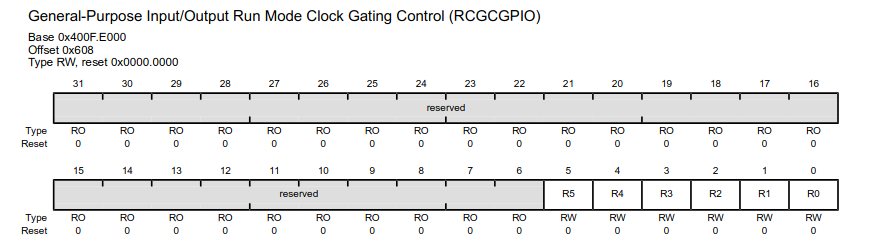
\includegraphics[scale=0.5]{images/tivac_datasheet_example.png}
\caption{Các thông số về RCGCGPIO của EK-TM4C123GH6PM ở trang 340}
\end{figure}

Dựa vào thông số này, nếu ta muốn kích hoạt clock cho GPIOF, và sau đó kích hoạt quyền ghi vào GPIOF ta sẽ viết một đoạn code C như sau:
\begin{listing}[ht]
\begin{ccode}
#include "TM4C123GH6PM.h"
SYSCTL->RCGCGPIO |= 0x20; // kich hoat clock cho GPIOF
GPIOF->LOCK = 0x4C4F434B; // unlockGPIOCR register
\end{ccode}
\caption{Ví dụ ghi trực tiếp vào các register sử dụng C}
\end{listing}

Các thao tác đọc ghi các thanh ghi này là các thao tác được cho là cấp thấp (low-level), thường chỉ các ngôn ngữ cấp thấp như C/C++ mới có thể thực hiện các thao tác này.
Các ngôn ngữ cấp cao thường không thể thực hiện trực tiếp các thao tác này, làm cho các ngôn ngữ này không thể lập trình nhúng được.
Rust là một ngôn ngữ cấp thấp,  ta cũng có thể thực hiện các thao tác tương tự như vậy nếu cần thiết.
Sau đây, tôi đưa ra một ví dụ về sử dụng Rust để thực hiện một thao tác tương tự trên một vi điều khiển STM32F1 để chứng minh điều này.
\begin{listing}[ht]
\begin{rustcode}
const GPIO_START: usize = 0x4001_1000;
const CRH_OFFSET: usize = 0x04;
const OUTPUT_MODE: u32 = 0b01;
const PUSH_PULL: u32 = 0b10;

unsafe {
    *((GPIOC_START + CRH_OFFSET) as *mut u32) = (OUTPUT_MODE << 20) | (PUSH_PULL << 22);
}
\end{rustcode}
\caption{Ví dụ ghi trực tiếp vào các register sử dụng Rust}
\end{listing}

Có thể dễ dàng nhận thấy rằng cách này rất khó viết, khó hiểu, tốn thời gian đọc datasheet và cực kỳ thiếu an toàn.
Để giải quyết các vấn đề này ta thường sử dụng các thư viện để abstract công việc này.
\section{Các thư viện abstract đề điều khiển vi điều khiển}
\subsection{Các thư viện abstract trong C}
Các thư viện thực hiện công việc abstract này trong C/C++ thường được cung cấp sẵn bởi nhà sản xuất.
Ta chỉ việc tải xuống các thư viện này, liên kết nó với phần mềm là có thể sử dụng được.
Ví dụ, để điều khiển EK-TM4C123GH6PM ta có thể tải xuống thư viện TivaWare \cite{tivac_tivaware} và sử dụng nó.
Sau khi được abstract, một chương trình khởi động port GPIO cũng như thiết lập cho nó có thể tương tự như sau:
\begin{listing}[ht]
\begin{ccode}
void setup_GPIOs()
{
     delay_ms(2000);
     GPIO_Clk_Enable(&GPIO_PORTF);
     GPIO_Config(&GPIO_PORTF,
                 (_GPIO_PINMASK_1 | _GPIO_PINMASK_2 | _GPIO_PINMASK_3),
                 _GPIO_DIR_OUTPUT,
                 (_GPIO_CFG_DIGITAL_ENABLE | _GPIO_CFG_DRIVE_8mA),
                 _GPIO_PINCODE_NONE);
}
\end{ccode}
\caption{Ví dụ về sử dụng một thư viện abstract trong C}
\end{listing}

Có thể thấy rằng, khi sử dụng các thư viện này ta có thể điều khiển các vi điều khiển một cách tương đối dễ dàng và an toàn.
Tuy nhiên, mặc dù đã được abstract, để có thể sử dụng điều khiển vi điều khiển một cách thích hợp ta vẫn phải đọc datasheet.
Ngoài ra, cách này có một nhược điểm lớn đó là các thư viện abstract này là platform-specific, điều này có nghĩa là chúng ta không thể sử dụng được thư viện này cho các các vi điều khiển khác.
Nếu ta muốn sử dụng một thư viện driver ngoài để tương tác với thiết bị ngoài, ta phải tự định nghĩa lại các thông số trong các thư viện này thì mới có thể sử dụng được nó.
Đây là một nhược điểm lớn đối với người lập trình nhúng, vì nếu muốn sử dụng nhiều vi điều khiển khác nhau thì ta phải học các thư viện viện khác nhau.

\subsection{Các thư viện abstract trong Rust}
Các thư viện thực hiện việc abstract này trong Rust được gọi là Peripheral Access Crates (PAC).
Vì các nhà sản xuất vi điều khiển không cung cấp sẵn các PAC nên người lập trình nhúng của Rust phải tự viết các thư viện này.
Tuy nhiên, việc viết các thư viện này là điều cực kỳ tốn công sức và dễ bị lỗi nên các nhà phát triển lập trình nhúng của Rust đi theo một hướng khác đó là sử dụng các file SVD được cung cấp sẵn bởi nhà sản xuất.
Các nhà sản xuất vi điều khiển ngoài việc cung cấp các file datasheet cho sản phẩm của mình thì thường còn cung cấp thêm các file SVD.
Các file SVD này mô tả các chức năng của vi điều khiển, các ngoại vi của nó, v.v.. theo các định dạng dành cho máy tính (như XML).
Các nhà phát triển lập trình nhúng của Rust đã thực hiện viết một chương trình là \mintinline{bash}{svd2rust} để thực tạo ra các crates (thư viện của Rust) một cách tự động từ các file SVD này.
Từ kết quả thu được, cộng thêm công việc sửa lại các artifact từ kết quả nếu có,
ta thu được các thư viện abstract này một cách tự động.
Ngoài ra, vì hệ thống ownership của Rust được compiler kiểm tra lúc biên dịch nên khi sử dụng các thư viện này, chúng ta cũng được hưởng lợi từ hệ thống ownership này!
Một ví dụ ở đây về lợi ích của hệ thống ownership là ta không thể thiết lập clock cho vi điều khiển nhiều lần.

Khi sử dụng PAC, ta có thể viết mã thực hiện công việc khởi động GPIO một cách dễ dàng hơn.
\begin{listing}[ht]
\begin{rustcode}
startup_gpio();
dp.GPIOC.crh.modify(|_r, w| {
    w.mode13().output()
     .cnf13().push_pull()
});
\end{rustcode}
\caption{Ví dụ về sử dụng một PAC trong Rust}
\end{listing}

Có thể thấy rằng, sử dụng PAC ta có thể viết các mã tương đối cao hơn như C mà vẫn không mất đi hiệu suất (zero-cost abstraction), an toàn hơn, cũng như được hưởng lợi từ hệ thống ownership của Rust.

Để giải quyết vấn đề về platform-specific, Rust đi theo một hướng khác.
Tuy nhiên, cũng như việc sử dụng các thư viện abstract trong C/C++, sử dụng PAC vẫn là platform-specific vì mỗi vi điều khiển sẽ có một PAC khác nhau.
Ngoài ra, mặc dù mã đã an toàn hơn (không trực tiếp sử dụng unsafe mà abstract qua PAC), tuy nhiên các lỗi về logic vẫn không được giải quyết.
Ví dụ, nếu ta không khởi động gpio \mintinline{bash}{startup_gpio();} mà trực tiếp thiết lập GPIO thì mã sẽ vẫn được biên dịch, tuy nhiên đến runtime thì ta mới phát hiện lỗi vì vi điều khiển không chạy!
Compiler không thể biết được ta có thực hiện công việc khởi động hệ thống có đúng hay không, mà nó chỉ có thể xác định được ta sử dụng các hàm tương tác với PAC đúng hay không.

\subsection{Hardware Abstraction Layer (HAL)}
Để giải quyết vấn đề này, Rust chọn cách là tiếp tục abstract PAC thành Hardware Abstraction Layer (HAL).
Trong C, ta cũng sử dụng các HAL để tương tác với vi điều khiển, nhưng trong Rust các HAL thường cao hơn các HAL trong C.
Khi sử dụng HAL của Rust, mã viết ra thường có cảm giác tương đương với mức độ abstraction trong lập trình arduino.
Ví dụ, khi ta sử dụng HAL \mintinline{bash}{stm32f1xx\_hal} để tương tác với vi điều khiển STM32F1 để khởi động GPIO, mã Rust sẽ được viết như sau:
\begin{listing}[ht]
\begin{rustcode}
let mut rcc = dp.RCC.constrain();
let mut gpioc = dp.GPIOC.split(&mut rcc.apb2);
let mut led = gpioc.pc13.into_push_pull_output(crh);
led.set_high();
\end{rustcode}
\caption{Ví dụ về sử dụng một PAC trong Rust}
\end{listing}

Giải thích qua mã:

Ở dòng 1, ta tạo một struct gồm các ngoại vi cơ bản (tương tự như \mintinline{bash}{startup_gpio}) để có thể sử dụng với HAL, ta làm cách này bằng cách sử dụng hàm \mintinline{bash}{constrain()}.
Sau đó để thiết lập GPIO, ta mượn struct này để thực hiện thiết lập GPIO bằng hàm \mintinline{bash}{split()}, một điểm lưu ý ở đây là muốn khởi tạo GPIO sử dụng HAL ta bắt buộc phải mượn struct RCC đã khởi tạo.
Nếu ví như ta không thể mượn được struct RCC, điều này có nghĩa là việc khởi chạy các ngoại vi bị lỗi.
Compiler có thể kiểm tra việc này lúc biên dịch và sẽ báo lỗi, tránh được việc tới runtime mới phát hiện ra lỗi của hệ thống.
Tương tự, ta tiếp tục mượn struct GPIOC để thiết lập LED (pin 13), và ta thiết lập nó ở chế độ push pull output.
Sau đó, để bật LED, ta chỉ việc sử dụng hàm \mintinline{bash}{set_high()}, có một điểm cần lưu ý ở đây là nếu ta không thiết lập pin ở chế độ output thì ta sẽ không có hàm \mintinline{bash}{set_high()}, đảm bảo cho an toàn nếu người lập trình thiết lập hệ thống sai.

Sử dụng HAL như cách này, ta có một interface với hệ thống ở cấp cao, dễ dàng viết mã, và đảm bảo được an toàn ngay từ lúc biên dịch.
Ngoài ra, nếu các HAL được viết tốt, ta hoàn toàn có thể dựa vào tài liệu hướng dẫn của HAL thay vì đọc datasheet!

\subsection{Các thiết bị ngoài}
Bước tiếp theo để lập trình một hệ thống nhúng là tương tác với các thiết bị bên ngoài.
Ở đây, tôi sẽ đưa ví dụ về cách sử dụng HAL để tương tác với cảm biến nhiệt độ, độ ẩm AHT20 \cite{aht20_datasheet}.
Đây là một HAL thực tế làm driver để điều khiển AHT20 trong Rust được viết bởi các nhà phát triển lập trình nhúng. \cite{hal_aht20}

\pagebreak
Ví dụ \ref{code:rust_hal_aht20_setup} sau đây là mã để thiết lập một thiết bị AHT20.

\begin{listing}[ht]
\begin{rustcode}
pub fn new(i2c: I2C, delay: D) -> Result<Self, Error<E>> {
    let mut dev = Self {
        i2c: i2c,
        delay: delay,
    };

    dev.reset()?;

    dev.calibrate()?;

    Ok(dev)
}
pub fn calibrate(&mut self) -> Result<(), Error<E>> {
    // Send calibrate command
    self.i2c.write(I2C_ADDRESS, &[0xE1, 0x08, 0x00])?;

    // Wait until not busy
    while self.status()?.contains(StatusFlags::BUSY) {
        self.delay.delay_ms(10);
    }

    // Confirm sensor is calibrated
    if !self.status()?.contains(StatusFlags::CALIBRATION_ENABLE) {
        return Err(Error::Uncalibrated);
    }

    Ok(())
}
\end{rustcode}
\caption{Ví dụ về sử dụng HAL để viết driver cho thiết bị ngoài trong Rust}
\label{code:rust_hal_aht20_setup}
\end{listing}

Để sử dụng HAL, ta thực thao tác đơn giản:

\begin{listing}[ht]
\begin{rustcode}
let mut dev = Aht20::new(i2c, hal::Delay).unwrap();
let (h, t) = dev.read().unwrap(); // h = humidity, t = temperature
\end{rustcode}
\caption{Ví dụ về sử dụng driver HAL để tương tác thiết bị ngoài trong Rust}
\end{listing}

Có thể thấy rằng, sử dụng HAL, ta có thể viết các mã ở mức rất cao, cực kỳ tiện lợi.
Các driver sử dụng type system của Rust để đảm bảo rằng các thiết bị được thiết lập đúng
(nếu thiết lập I\textsuperscript{2}C sai thì sẽ không thể thiết lập được thiết bị AHT20).
Hệ thống ownership đảm bảo rằng các pin cũng như các ngoại vi hệ thống như I\textsuperscript{2}C không bị dùng chung ở bất cứ thời điểm nào.

Tuy nhiên, ta vẫn có thể dễ dàng nhận ra nhiều nhược điểm của HAL.
Một vài nhược điểm lớn có thể được nêu ra như:

\begin{itemize}
    \item Toàn bộ những HAL này được viết thủ công để abstract PAC.
        Không có HAL nào được viết tự động từ PAC cả.
        Điều này dẫn đến hai vấn đề khác là chất lượng của các HAL này phụ thuộc phần lớn vào người thiết kế các HAL này.
        Một vấn đề khác là vì viết các HAL là công việc thủ công nên không phải toàn bộ các chức năng của vi xử lý được định nghĩa trong PAC sẽ có lớp abstraction HAL.
    \item Vì mỗi HAL sẽ có một API để tương tác với vi điều khiển khác nhau nên người dùng thiết kế hệ thống nhúng sử dụng nhiều vi điều khiển khác nhau thì họ vẫn phải học cách sử dụng nhiều HAL khác nhau.
    \item Đến đây, ta vẫn chưa giải quyết được vấn đề về platform specific. Nếu muốn crate driver tương tác với thiết bị ngoài hỗ trợ cho vi xử lý nào đó, người lập trình HAL phải tự viết một HAL riêng cho các driver này. \label{list:hal_prob}
\end{itemize}

\subsection{Embedded HAL}
Để giải quyết vấn đề này, các nhà lập trình nhúng của Rust dựa trên một tính năng có sẵn trong Rust đó là sử dụng \mintinline{bash}{traits} để tái sử dụng lại các thuộc tính được định nghĩa sẵn.
Crate dùng để định nghĩa các trait cho ngoại vi thông dụng (như GPIO, Timer, SPI, UART, v.v..) này được gọi là \mintinline{bash}{Embedded HAL} \cite{embedded_hal}.

Sau khi có được các trait định nghĩa từ Embedded HAL, các nhà lập trình nhúng viết HAL cho các vi điều khiển riêng biệt tái sử dụng lại các trait này để viết HAL cho vi điều khiển của mình.
Sau khi hoàn thành, những người viết driver cho các thiết bị ngoài trong Rust chỉ việc tái sử dụng lại các trait được định nghĩa trước này.
Bất cứ HAL cho các vi điều khiển nào mà đã tái sử dụng các trait này thì chắc chắn driver sẽ hoạt động cho vi điều khiển đó mà không cần phải chỉnh sửa lại crate driver.
Ta chỉ việc viết driver một lần duy nhất và toàn bộ tất cả các HAL cho vi điều khiển đều có thể sử dụng driver này.
Đây chính là điểm then chốt trong hệ sinh thái lập trình nhúng của Rust.

Để xem một ví dụ, ta xem lại ví dụ về driver AHT20 của Rust (ví dụ \ref{code:rust_hal_aht20_setup}).
Ở đây, tôi đã thêm phần tái sử dụng trait trong ví dụ mới này.
Có thể thấy rằng, driver này đã tái sử dụng hai trait từ Embedded HAL đó là \mintinline{bash}{delay} và \mintinline{bash}{i2c}.
Điều này có nghĩa là bất cứ HAL cho vi điều khiển nào cũng tái sử dụng hai trait này từ Embedded HAL đều có thể sử dụng crate driver này một cách trực tiếp mà không cần thay đổ bất cứ thông số nào.
\begin{listing}[ht]
\begin{rustcode}
use embedded_hal::blocking::{delay::DelayMs, i2c::{Write, WriteRead}};
pub fn new(i2c: I2C, delay: D) -> Result<Self, Error<E>> {
\end{rustcode}
\caption{Ví dụ về tái sử dụng trait để viết driver trong Rust}
\end{listing}

Đến đây, ta đã có được một hệ thống hoàn chỉnh, sẵn sàng để áp dụng vào viết các hệ thống nhúng một cách nhanh gọn, an toàn và dễ dàng.
Ở chương tiếp theo, tôi đi vào thực hiện áp dụng Rust để viết một số hệ thống nhúng và chạy các chương trình này trên một vi điều khiển thực để minh họa cách chúng ta có thể áp dụng Rust để lập trình nhúng như thế nào.

\chapter{Ứng dụng ngôn ngữ Rust}
\section{Chọn vi xử lý để thực hiện lập trình nhúng trong Rust}
Trước khi thực hiện lập trình nhúng cho bất kỳ hệ thống nào, ta phải chọn một vi điều khiển phù hợp cho hệ thống đó trước.

Trước hết, em đưa ra một số vi xử lý thông dụng, phù hợp, được sử dụng để giảng dạy về lập trình hệ nhúng ở trường Đại học Bách Khoa TP.HCM, so sánh chúng và từ đó chọn một vi xử lý phù hợp với nhu cầu.
\subsection{Một số vi xử lý thông dụng}
\subsubsection{MSP-EXP430G2 Evaluation board}
\begin{figure}[ht]
\centering
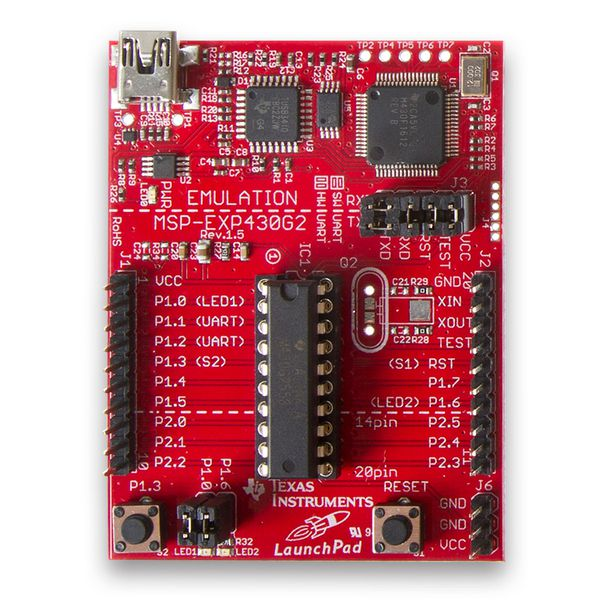
\includegraphics[scale=0.35]{images/launchpad-mspexp430g2-02.jpg}
\caption{MSP-EXP430G2}
\end{figure}
\clearpage

MSP-EXP430G2 \cite{msp430_datasheet} (hay MSP430) là dòng vi điều khiển của Texas Instrument (TI), 16 bit, kiến trúc RISC được thiết kế đặc biệt cho siêu năng lượng thấp.

\textbf{Một số hiệu năng nổi bật của MSP430}
\begin{itemize}
    \item CPU 16 bit tốc độ \si{16\MHz}.
    \item 16 KB Flash.
    \item 512B SRAM.
\end{itemize}

\textbf{Ưu điểm}: Giá thành rẻ, nhỏ gọn, đầy đủ các ngoại vi thông dụng. Có bộ thư viện phong phú dễ dàng thực hiện lập trình nhúng trên nhiều lĩnh vực.

\textbf{Nhược điểm}: Khá ít bộ nhớ SRAM, cũng như tốc độ CPU còn hạn chế, và CPU chỉ hỗ trợ tính toán 16 bit nên sẽ khó có thể thực hiện tính toán nặng trên MSP430.

\subsubsection{STM32F103C8T6 - Blue Pill}
\begin{figure}[ht]
\centering
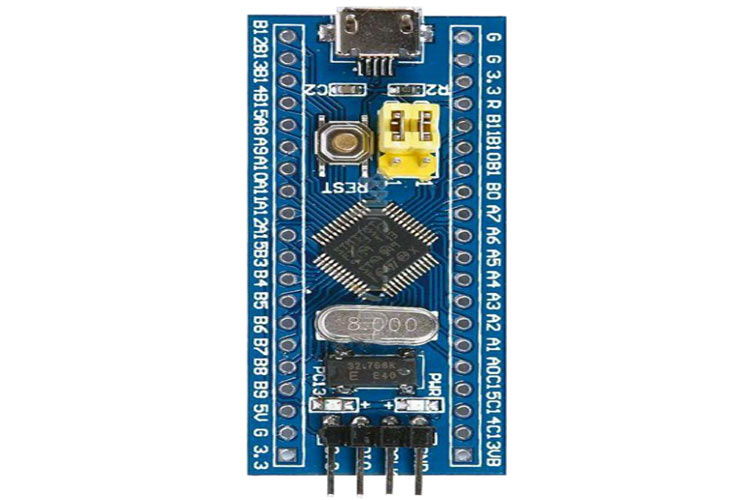
\includegraphics[scale=0.35]{images/STM32-Blue-Pill-Development-Board.jpg}
\caption{STM32 Blue Pill}
\end{figure}
STM32F103C8T6 \cite{blue_pill_datasheet} (hay Blue Pill) là một vi xử lý rất thông dụng của ST-Microelectronics, sử dụng CPU Arm-Cortex M3, 32 bit với giá thành rẻ.

\textbf{Một số hiệu năng nổi bật của Blue Pill}
\begin{itemize}
    \item CPU ARM-Cortex M3 32 bit tốc độ \si{72\MHz}, 1.25 DMIPS/MHz.
    \item 128 KB Flash.
    \item 20 KB SRAM.
\end{itemize}

\textbf{Ưu điểm}: Giá thành rẻ, nhỏ gọn, đầy đủ các ngoại vi thông dụng. CPU mạnh mẽ. Kèm theo một số ngoại vi khác như RTC.

\textbf{Nhược điểm}: Vì Blue Pill sử dụng CPU ARM-Cortex M3 nên một số tính năng tính toán nặng như DSP sẽ không được phần cứng hỗ trợ. Ngoài ra, ta không thể flash trực tiếp chương trình lên Blue Pill được mà phải thông qua một Bootloader như ST-Link/V2 \cite{stlinkv2_datasheet}.

\subsubsection{Arduino Uno R3}
\begin{figure}[ht]
\centering
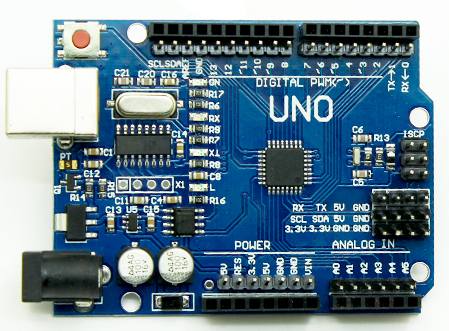
\includegraphics[scale=0.75]{images/Arduino-Uno-R3-SMD.jpg}
\caption{Arduino Uno R3}
\end{figure}

Arduino Uno R3 \cite{arduino_datasheet} là loại phổ biến và dễ sử dụng nhất trong các dòng Arduino hiện nay cũng như tương thích với nhiều Arduino Shield.

\textbf{Một số hiệu năng nổi bật của Arduino Uno R3}
\begin{itemize}
    \item CPU ATmega328P 8 bit tốc độ \si{16\MHz}.
    \item 32 KB Flash.
    \item 1 KB EEPROM.
    \item 2 KB SRAM.
\end{itemize}

\textbf{Ưu điểm}: Giá thành rẻ, nhỏ gọn, đầy đủ các ngoại vi thông dụng.

Có rất nhiều thư viện abstraction C/C++ chất lượng cao, dễ sử dụng.

\textbf{Nhược điểm}: Hiệu năng tính toán của Arduino Uno R3 tương đối hạn chế.

AVR \mintinline{bash}{avr-unknown-gnu-atmega328} là đối tượng bậc 3 của bộ compiler trong Rust \cite{rustc_book}, vì vậy lập trình trên vi điều khiển này sẽ gặp nhiều chướng ngại vật, khó có thể đánh giá khách quan về hệ thống.

\clearpage
\subsubsection{EK-TM4C123G}
\begin{figure}[ht]
\centering
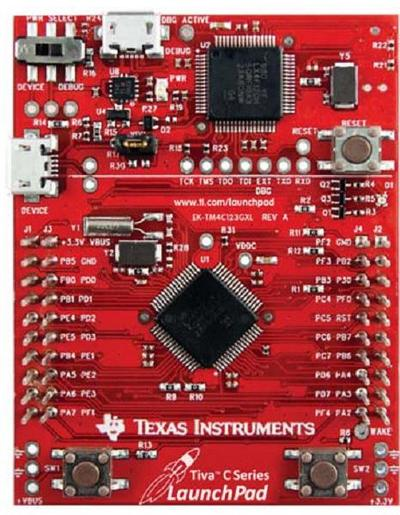
\includegraphics[scale=0.5]{images/kit_tivac.jpg}
\caption{Evaluation Kit EK-TM4C123G}
\end{figure}

EK-TM4C123G \cite{tivac_datasheet} (hay kit Tiva C launchpad) được phát triển bởi tập đoàn Texas Instruments để thay thế cho sản phẩm Stellaris Launchpad đã dừng sản xuất trước đó.
Dòng Tiva C 32-bit được sử dụng trong đề tài này có một thiết kế hiện đại cùng tập lệnh phong phú và hệ sinh thái về code nhúng giàu có
đã đẩy nhanh việc giảng dạy về lập trình nhúng nói chung trong môi trường trường học cũng như cũng đủ mạnh mẽ để có thể phát triển thêm lên để sử dụng trong môi trường công nghiệp hiện đại.

\textbf{Một số hiệu năng nổi bật của Tiva C launchpad}
\begin{itemize}
    \item CPU ARM-Cortex M4F 32 bit tốc độ \si{80\MHz}, 1.25 DMIPS/MHz.
    \item 256 KB Flash.
    \item 32 KB SRAM.
    \item 2 KB EEPROM.
\end{itemize}

\textbf{Ưu điểm}: Giá thành rẻ, nhỏ gọn, mạnh mẽ. Có bộ thư viện phong phú dễ dàng thực hiện lập trình nhúng trên nhiều lĩnh vực.
Khả năng hoạt động với chế độ tiết kiệm điện để hoạt động liên tục, phù hợp cho việc áp dụng cho môi trường thực tiễn.

\textbf{Nhược điểm}: Giá thành vẫn còn đắt hơn so với một số thiết bị STM32 với cùng hiệu năng. (khoảng 350000 VNĐ ở thời điểm tháng 06/2021)

\clearpage
\subsubsection{STM32F411 Discovery}
\begin{figure}[ht]
\centering
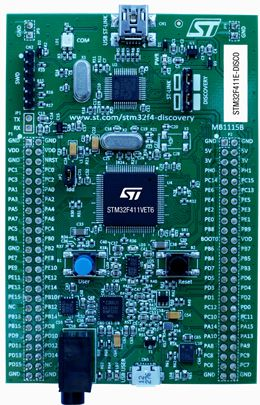
\includegraphics[scale=0.5]{images/en-stm32f411e-disco.jpg}
\caption{STM32F411 Discovery}
\end{figure}

STM32F411 \cite{discovery_datasheet} (hay STM32 Discovery) là một phiên bản nâng cấp của kit STM32F407 Discovery được sử dụng rất phổ biển hiện nay trong các nghiên cứu về dòng ARM STM32F4.
Kit có tích hợp sẵn mạch nạp ST-Link/V2, các ngoại vi như cảm biến gia tốc, từ trường, audio, v.v..

\textbf{Một số hiệu năng nổi bật của STM32 Discovery}
\begin{itemize}
    \item CPU ARM-Cortex M4 + DSP Core 32 bit tốc độ \si{100\MHz}, 1.25 DMIPS/MHz.
    \item 512 KB Flash.
    \item 128 KB SRAM.
\end{itemize}

\textbf{Ưu điểm}: Các thông số hiệu năng cực kỳ mạnh mẽ, kèm theo DSP Core cũng như tích hợp một số ngoại vi khác như cảm biến gia tốc, từ trường, audio, v.v..

\textbf{Nhược điểm}: Giá thành tương đối đắt (khoảng 500.000 VNĐ ở thời điểm tháng 06/2021).

\subsubsection{Raspberry Pi 3 Model B+}
\begin{figure}[ht]
\centering
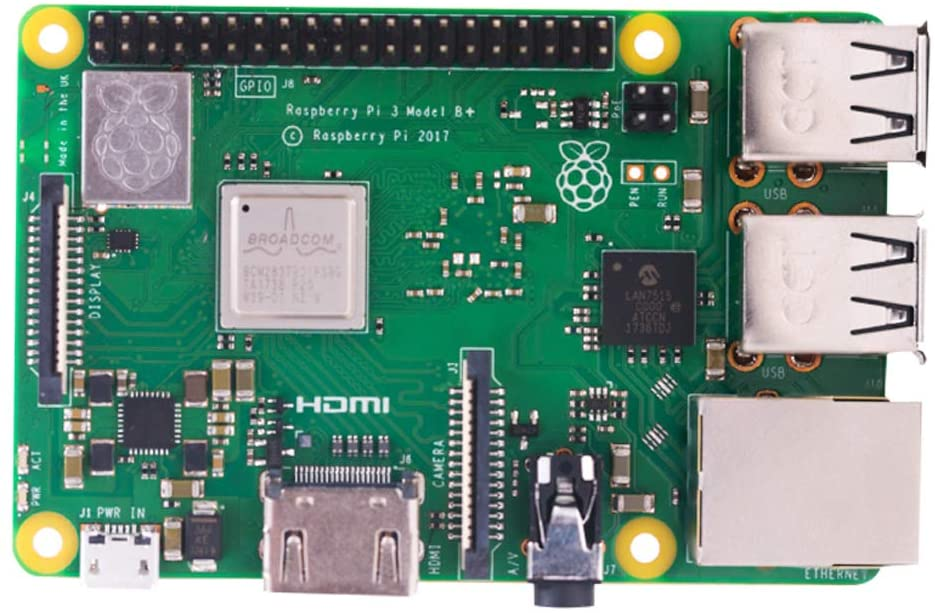
\includegraphics[scale=0.25]{images/raspberry-pi-model-3bplus.jpg}
\caption{Raspberry Pi 3 Model B+}
\end{figure}
Máy tính Raspberry Pi 3 Model B+ \cite{raspberry_datasheet} là một trong những sản phẩm tương đối mới, nổi bật với 4 nhân 64 bit CPU ARM-Cortexv8 với tốc độ lên đến 1.4 GHz.
Máy tính Raspberry Pi 3 Model B+ đủ mạnh để có thể chạy được một hệ điều hành như Linux.

\textbf{Một số hiệu năng nổi bật của Raspberry Pi 3 Model B+}
\begin{itemize}
    \item Quad-core CPU ARM-Cortex-A53 64 bit tốc độ \si{1.2\GHz}.
    \item 1 GB RAM.
    \item Đi kèm với VideoCore IV multimedia/3D graphic core.
\end{itemize}

\pagebreak
\textbf{Ưu điểm}: Có hiệu năng vượt trội hơn hẳn tất cả các vi điều khiển đã liệt kê trước.

Thư viện hỗ trợ cho Raspberry Pi có thể được xem là một trong những thư viện đầy đủ nhất.

Raspberry Pi 3 Model B+ đủ mạnh để có thể chạy hệ điều hành Linux nên ta có thể lập trình nhúng cực kỳ dễ dàng và hiệu quả.

\textbf{Nhược điểm}: Giá thành đắt. Tại thời điểm tháng 06/2021 thì giá thành của một kit Raspbery Pi 3 Model B+ là khoảng 1100000 VNĐ chưa kèm phụ kiện.

\subsection{Lựa chọn vi điều khiển}

Ở đây, để thực hiện ứng dụng Rust cho một hệ thống nhúng thực tế, em đưa ra một số yêu cầu để thử nghiệm ngôn ngữ này.

\begin{itemize}
    \item Vi điều khiển này có đầy đủ các chức năng của một vi điều khiển thông dụng, để ta có thể dễ dàng thử nghiệm toàn bộ những ngoại vi cơ bản.
    \item Vi điều khiển này được hỗ trợ tương đối tốt, cả trong C lẫn Rust để ta có thể dễ dàng so sánh kết quả trong quá trình thiết kế hệ thống nhúng.
    \item Vì Rust là một ngôn ngữ cấp thấp, em muốn thử nghiệm tính toán nặng trên vi điều khiển để kiểm tra về tốc độ của Rust trong một hệ thống thực tế.
    \item Giá thành tương đối rẻ.
        Trong lập trình nhúng, thiết kế các hệ thống với những giới hạn nhất định về phần cứng cũng như về giá thành của hệ thống là một công việc mà người thiết kế hệ thống thường xuyên gặp phải.
        Vì vậy, Rust phải hỗ trợ những vi điều khiển giá rẻ, không được giới hạn bởi các vi điều khiển cao cấp.
\end{itemize}

Dựa trên các yêu cầu này, có thể thấy có hai lựa chọn về vi xử lý để thực hiện những yêu cầu này là kit Tiva C và kit STM32 Discovery.

Ở đây, em quyết định chọn kit Tiva C làm đối tượng để nghiên cứu trong đề tài này vì giá thành của nó rẻ hơn so với kit STM32 Discovery.

\section{Viết phần mềm nhúng cho vi điều khiển trong Rust}
Trước khi thực hiện viết chương trình nhúng cho vi điều khiển, ta cần chuẩn bị một số công cụ để thực hiện điều này.

\begin{itemize}
    \item Các công cụ của Rust: chi tiết cài đặt có thể xem tại website chính thức Rust Programming Language \cite{rust_website}.
    \item Cargo clone: cài đặt thông qua \mintinline{bash}{cargo install cargo-clone} \cite{cargo_clone}.
    \item Một số các công cụ biên dịch mã cho đối tượng ARM:

    \mintinline{bash}{arm-none-eabi-gcc arm-none-eabi-ar arm-none-eabi-objcopy}
    \item Công cụ flash cho Tiva C: \mintinline{bash}{lm4flash} \cite{lm4tools}.
    \item GDB cho đối tượng ARM: \mintinline{bash}{gdb-arm-none-eabi} \cite{gdb_website}.
    \item OpenOCD: \mintinline{bash}{openocd} \cite{openocd_website}.
\end{itemize}

Ở đây, vì kit Tiva C có một BSP là \mintinline{bash}{stellaris-launchpad} \cite{stellaris_launchpad_bsp} nên em sẽ sử dụng crate này để đấy nhanh tiến độ thực hiện lập trình. \label{lbl:tivac_bsp}

Trước hết, ta tham khảo cấu trúc của crate \mintinline{bash}{stellaris-launchpad} qua ví dụ \ref{lst:stellaris_launchpad_structure}.

\begin{listing}
\dirtree{%
.1 stellaris-launchpad/.
.2 .cargo.
.2 examples.
.2 src.
.2 .gdbinit.
.2 Cargo.lock.
.2 Cargo.toml.
.2 build.rs.
.2 memory.x.in.
}
\caption{Cấu trúc của crate BSP stellaris-launchpad}
\label{lst:stellaris_launchpad_structure}
\end{listing}

Ta thấy nó tương tự với cấu trúc một dự án Rust cơ bản (xem trang \pageref{lbl:basic_rust_proj_structure}), nhưng có thêm một số file khác.
Em đi tiến hành phân tích về công dụng của các file này.

\textbf{.gdbinit}

File này chứa các lệnh của GDB sẽ thực hiện khi khởi động GDB \cite{gdbinit}.

\textbf{build.rs}

Một số thư viện cần phải biên dịch thêm một số mã nguồn khác (như C), một số khác cần phải link với các thư viện C trên hệ thống hay biên dịch từ mã nguồn.

Vì \mintinline{bash}{cargo} không thể thực hiện những điều này nên file \mintinline{bash}{build.rs} được sử dụng để thông báo cho \mintinline{bash}{cargo} rằng nó sẽ không thực hiện biên dịch mã trực tiếp mà sẽ thông qua một số bước khác được định nghĩa trong file này \cite{cargo_book}.

\textbf{memory.x}

File này chứa thông số về địa chỉ FLASH và địa chỉ RAM cũng như độ lớn của chúng.

Ví dụ \ref{lst:memory_x} là nội dung file \mintinline{bash}{memory.x} của crate BSP \mintinline{bash}{stellaris-launchpad}.

\begin{listing}[ht]
\begin{plaintext}
MEMORY
{
    FLASH (rx) : ORIGIN = 0x00000000, LENGTH = 0x00040000
    RAM (rwx) : ORIGIN = 0x20000000, LENGTH = 0x00008000
}
\end{plaintext}
\caption{Một ví dụ về file memory.x}
\label{lst:memory_x}
\end{listing}

Dựa theo hướng dẫn của crate, ta thấy rằng, các dự án sẽ được viết và đặt trong thư mục \mintinline{bash}{examples}.

Biên dịch sử dụng lệnh \mintinline{bash}{cargo build --example <name> --release}.

Chuyển thành dạng binary sử dụng lệnh \mintinline{bash}{arm-none-eabi-objcopy -O binary tgt dst}

Và cuối cùng là flash file binary lên kit bằng lệnh \mintinline{bash}{lm4flash dst.bin}

Em tiến hành viết một số chương trình có độ khó từ đơn giản đến phức tạp để thử nghiệm Rust trên Tiva C.

\subsection{Chương trình nháy LED}\label{lbl:rust_blinky}
Chương trình nháy LED được xem là chương trình đơn giản nhất trong một hệ thống nhúng.
Em tiến hành thực hiện viết một chương trình nháy LED để làm quen với cách làm việc với một đề tài hệ thống nhúng trong Rust.

Để thực hiện một chương trình nháy LED, em trước tin thực hiện trực tiếp thông qua HAL của kit Tiva C \cite{tm4c_hal}.
Chương trình có nội dung như trong ví dụ \ref{code:tivac_hal_blinky} sau.

\begin{listing}[ht]
\begin{rustcode}
#![no_std]
#![no_main]

use panic_halt as _;

use cortex_m_rt::entry;
use tm4c123x_hal::{self as hal, prelude::*};

#[entry]
fn main() -> ! {
    let p = hal::Peripherals::take().unwrap();

    let mut sc = p.SYSCTL.constrain();
    sc.clock_setup.oscillator = hal::sysctl::Oscillator::Main(
        hal::sysctl::CrystalFrequency::_16mhz,
        hal::sysctl::SystemClock::UsePll(hal::sysctl::PllOutputFrequency::_80_00mhz),
    );
    let clocks = sc.clock_setup.freeze();

    let portf = p.GPIO_PORTF.split(&sc.power_control);
    let mut led = portf.pf1.into_push_pull_output();

    let mut delay = hal::delay::Delay::new(core_peripherals.SYST, &clocks);

    loop {
        led.set_high();
        delay.delay_ms(500u32);
        led.set_low();
        delay.delay_ms(500u32);
    }
}
\end{rustcode}
\caption{Ví dụ blinky sử dụng Tiva C HAL}
\label{code:tivac_hal_blinky}
\end{listing}

Em phân tích một vài điểm chưa được giải thích ở trong các phần trước từ ví dụ này.

\begin{itemize}
    \item Đầu tiên là hai thuộc tính \mintinline{rust}{#[no_std]} và \mintinline{rust}{#[no_main]} được đặt ở đầu chương trình.

        \mintinline{rust}{#[no_std]} như đã phân tích ở phần \ref{lbl:no_std_crates} (trang \pageref{lbl:no_std_crates}), ở đây được đặt ra để báo với compiler là chương trình này không sử dụng thư viện std.

    \mintinline{rust}{#[no_main]} thông báo với compiler rằng chương trình này sẽ không sử dụng symbol \mintinline{bash}{main} thông thường để làm entry point. Thông thường, một chương trình Rust suy đoán một số thông số từ môi trường mà chương trình sẽ chạy trên. Tuy nhiên ở trong môi trường nhúng, các thông số này có thể không đúng, vì vậy để chương trình được biên dịch chính xác ta cần phải có thuộc tính này \cite{rust_reference, embedonomicon}.

    \item \mintinline{rust}{use panic_halt as _;} đoạn mã này tạo một hàm \mintinline{bash}{panic} để khi chương trình gặp lỗi thì nó sẽ chuyển sang chạy một vòng lặp vô hạn trong hàm này.
    \item \mintinline{rust}{#[entry]} thông báo với compiler đây là điểm entry của chương trình.
        Thuộc tính này được lấy từ crate \mintinline{bash}{cortex-m-rt-macros} để từ đó kết hợp với file \mintinline{bash}{memory.x} để flash chương trình đúng vào địa chỉ dùng cho bộ nhớ FLASH \cite{cortex_m_rt}.
\end{itemize}

Từ trong chương trình main, các lệnh để thực hiện khởi động ngoại vi, thiết lập xung clock có thể thấy tương đối tương tự như ta sử dụng các hàm trong C để thực hiện các thao tác này, chỉ có một điểm ở đây cần chỉ ra đó là khi khởi động LED (pin PF1 trên kit), ta phải đặt biến này ở dạng mutable vì khi thực hiện nháy LED thì ta phải thay đổi trạng thái ON/OFF của LED, nếu không khởi động ở dang mutable thì chương trình khi biên dịch sẽ gặp lỗi. Điều này tương tự với biến delay.

Có thể thấy rằng, khi có HAL, thực hiện một chương trình đơn giản như nháy LED là tương đối đơn giản, dễ hiểu và nhanh chóng.
Giao diện này là ở mức khá cao, có thể nói là cao hơn so với thư viện HAL TivaWare \cite{tivac_tivaware}, khá tương đồng với cách sử dụng HAL như trong IDE của Arduino.

Tuy nhiên, ta vẫn có thể đi lên một nấc abstraction cao hơn nữa nhờ sử dụng BSP của kit Tiva C (đã giới thiệu ở trang \pageref{lbl:tivac_bsp}).
Ta thực hiện viết viết một file \mintinline{bash}{blinky.rs} với nội dung như trong ví dụ \ref{code:tivac_bsp_blinky}.

\begin{listing}[ht]
\begin{rustcode}
#![no_std]
#![no_main]

extern crate embedded_hal;
extern crate stellaris_launchpad;
extern crate tm4c123x_hal;

use embedded_hal::blocking::delay::DelayMs;
use embedded_hal::digital::v2::OutputPin;

#[no_mangle]
pub fn stellaris_main(mut board: stellaris_launchpad::board::Board) {
    let mut delay = tm4c123x_hal::delay::Delay::new(
        board.core_peripherals.SYST,
        stellaris_launchpad::board::clocks(),
    );

    loop {
        board.led_red.set_high().unwrap();
        delay.delay_ms(500u32);
        board.led_red.set_low().unwrap();
        delay.delay_ms(500u32);
    }
}
\end{rustcode}
\caption{Ví dụ blinky sử dụng Tiva C BSP}
\label{code:tivac_bsp_blinky}
\end{listing}

Ở đây, khi sử dụng BSP ta thấy việc nháy LED còn đơn giản hơn nữa vì BSP đã thực hiện các việc như khởi động kit, thiết lập clock, các ngoại vi cơ bản (như các LED trên kit) cho chúng ta và trả về một biến mutable là \mintinline{bash}{board} để ta mượn và sử dụng nó.

\subsection{Sử dụng một vài ngoại vi đơn giản}\label{lbl:rust_peripheral}
Sau khi đã nắm được cách viết một chương trình cơ bản, em tiếp tục thực hiện tương tác với một vài ngoại vi cơ bản của kit.
Ở ví dụ này, em chọn hai ngoại vi đó là UART và bộ Timer trên kit để tạo xung PWM điều khiển LED của kit.
Nội dung của chương trình người đọc có thể tham khảo ở phần phụ lục \ref{lbl:appendix_rust_peripheral} (trang \pageref{lbl:appendix_rust_peripheral}).

Một vài hình về kết quả thực hiện có thể xem ở các hình \ref{fig:cycle_kit}, \ref{fig:cycle_uart_out}, \ref{fig:cycle_uart_read}.

\begin{figure}[ht]
\centering
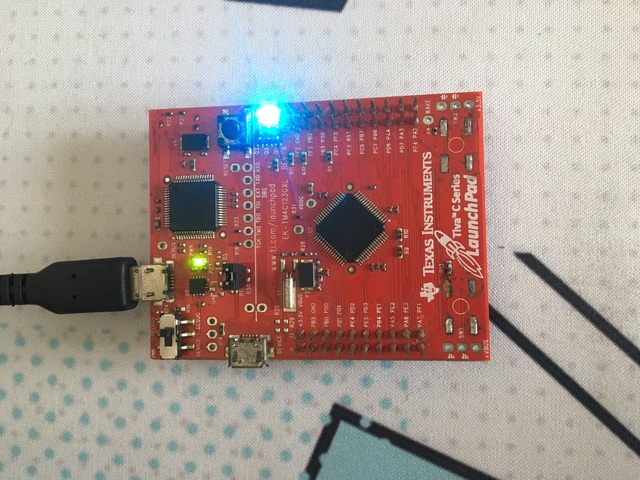
\includegraphics[scale=0.4]{images/cycle_kit.jpg}
\caption{LED cycle trên kit sử dụng Timer để tạo xung PWM}
\label{fig:cycle_kit}
\end{figure}

\begin{figure}[ht]
\centering
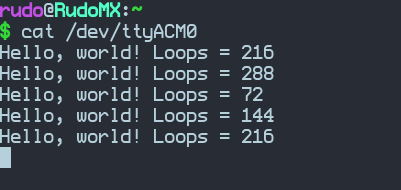
\includegraphics[scale=0.7]{images/cycle_uart_out.png}
\caption{Đọc thông tin từ kit sử dụng UART}
\label{fig:cycle_uart_out}
\end{figure}

\begin{figure}[ht]
\centering
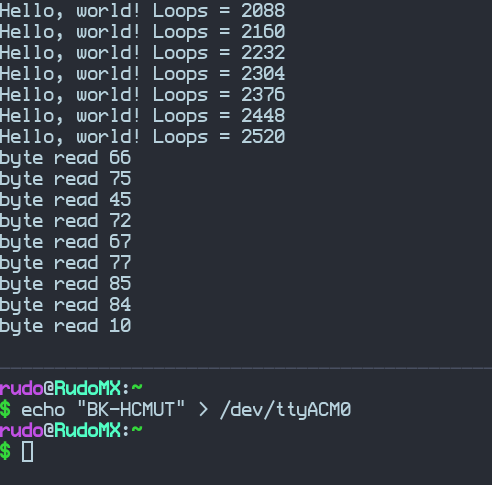
\includegraphics[scale=0.5]{images/cycle_uart_read.png}
\caption{Truyền thông tin cho kit sử dụng UART}
\label{fig:cycle_uart_read}
\end{figure}

\clearpage
\subsection{Tương tác với một vài thiết bị ngoài}\label{lbl:rust_mfrc522}
Sau khi đã làm quen với kit và các ngoại vi trên kit, bước tiếp theo em thực hiện tương tác với một số thiết bị ngoài.
Ở đây, em chọn 2 thiết bị là LCD 1602 \cite{lcd_datasheet} và module MFRC522 \cite{mfrc522_datasheet} thực hiện mô phỏng một hệ thống khóa cửa đơn giản.

Trước khi thực hiện hệ thống, em thực hiện gia công một mạch in đơn giản để thuận tiện hơn cho việc thực hiện hệ thống.
Schematic của hệ thống được trình bày ở hình \ref{fig:schematic}.
Kết quả thực hiện PCB và kết quả của hệ thống có thể xem ở các hình \ref{fig:pcb_routing}, \ref{fig:pcb_out}, \ref{fig:system}.

\begin{figure}[ht]
\centering
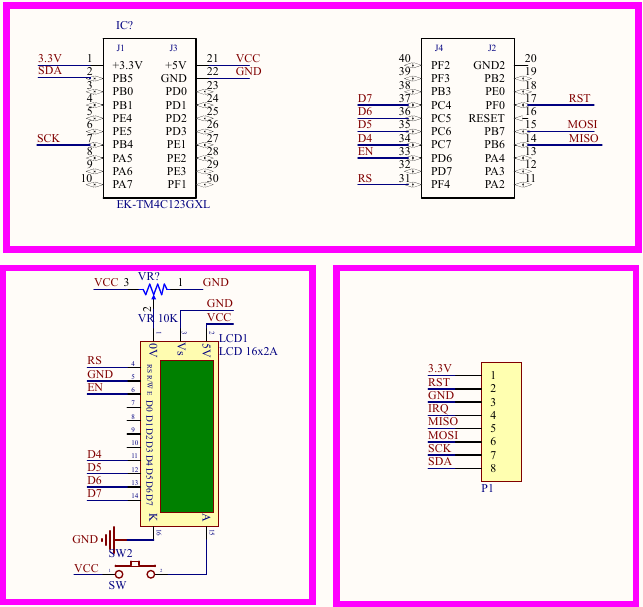
\includegraphics[scale=0.75]{images/schematic.png}
\caption{Schematic của hệ thống RFID}
\label{fig:schematic}
\end{figure}

\begin{figure}[ht]
\centering
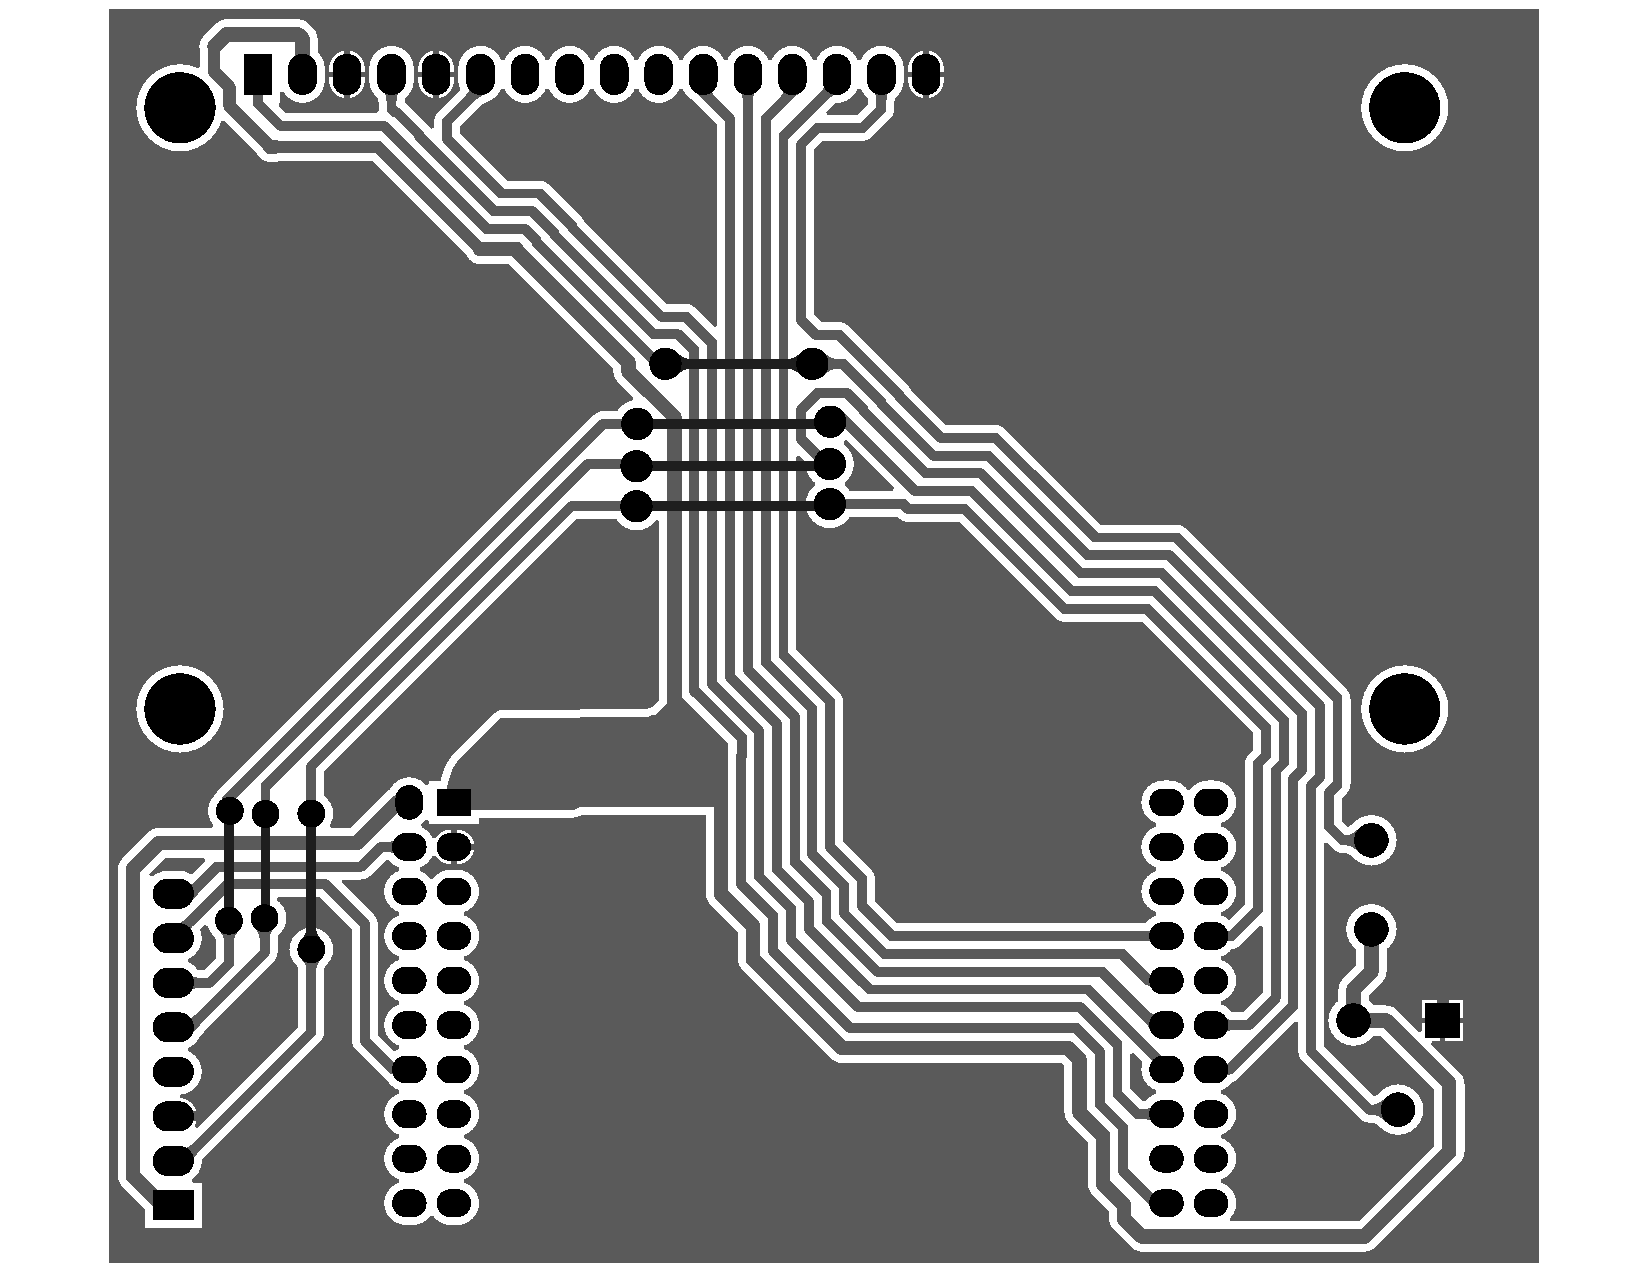
\includegraphics[scale=0.35]{images/routed.pdf}
\caption{Kết quả mạch sau khi thực hiện routing}
\label{fig:pcb_routing}
\end{figure}

\begin{figure}[ht]
\centering
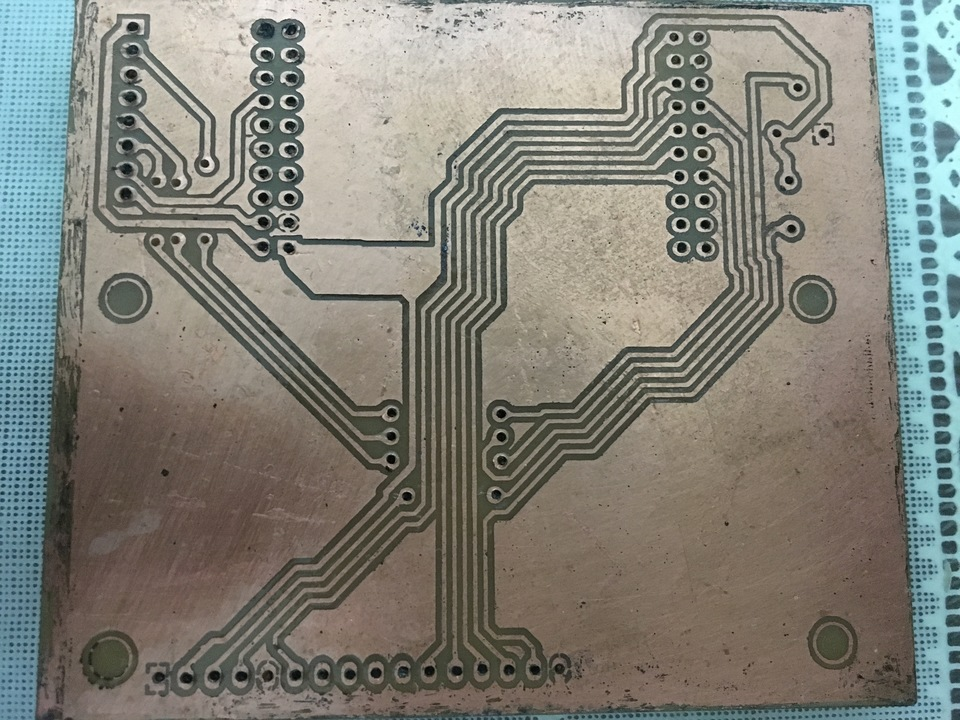
\includegraphics[scale=0.3]{images/board_output.jpg}
\caption{Kết quả mạch in}
\label{fig:pcb_out}
\end{figure}

\begin{figure}[ht]
\centering
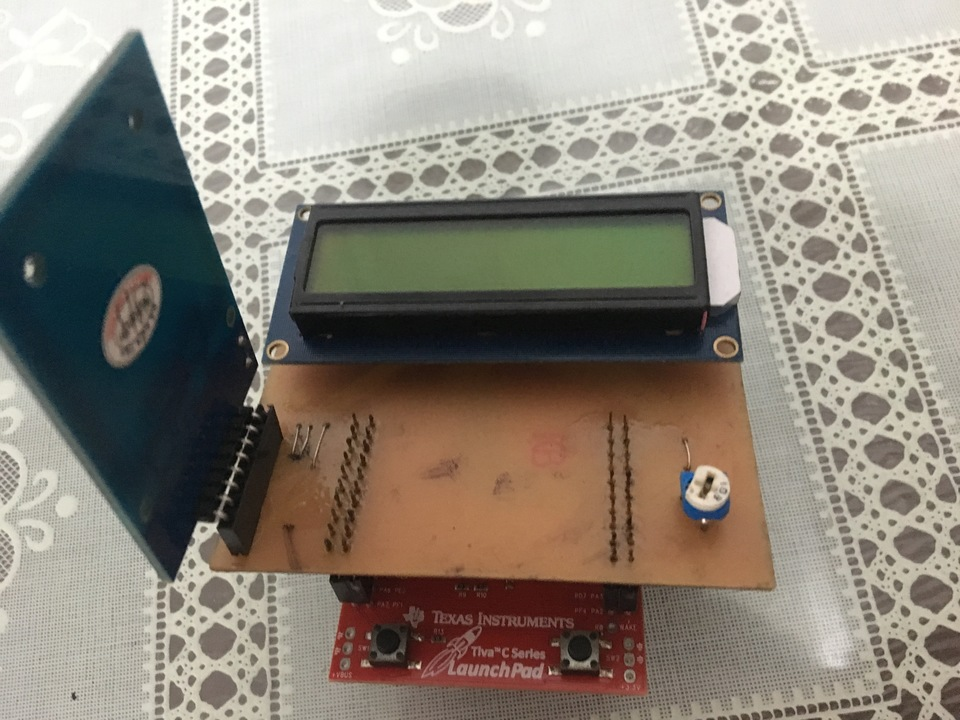
\includegraphics[scale=0.3]{images/board_finish.jpg}
\caption{Kết quả PCB đã gắn các linh kiện}
\label{fig:system}
\end{figure}

Lưu đồ giải thuật của chương trình được trình bày ở hình \ref{fig:rc522_flow}.

\begin{figure}[ht]
\centering
\begin{tikzpicture}[scale=0.75, every node/.style={scale=0.75}]
\tikzset{startstop/.style = {draw, rectangle, rounded corners, align=center, minimum width=3cm, minimum height=1cm}, >= latex,}
\tikzset{process/.style = {draw, rectangle, align=center, minimum width=3cm, minimum height=1cm}, >= latex,}
\tikzset{decision/.style = {draw, diamond, align=center, minimum width=3cm, minimum height=1cm}, >= latex,}
% Main nodes
\node (start) [startstop] {Bắt đầu};
\node (init) [process] [below=1cm of start] {Initialize hệ thống \\ Chọn chip slave};
\node (lcd_default) [process] [below=1cm of init] {Hiển thị dòng chữ \\ "Scan your card" ra LCD};
\node (card_check) [decision] [below=1cm of lcd_default] {Kiểm tra \\ có thẻ \\ được quét \\ không?};
\node (data_process) [process] [below=1cm of card_check] {Xử lý dữ liệu \\ đọc từ thẻ};
\node (led_blink) [process] [below=1cm of data_process] {Chớp LED trên board \\ báo hiệu đã đọc thẻ};
% Various coordinates
\coordinate[left=2cm of led_blink] (left_out);
\coordinate[above=0.5cm of card_check] (loop);
\coordinate[right=1cm of card_check] (right_card);
\coordinate[right=1cm of loop] (right_loop);
% Connectors
\draw [->] (start) -- (init);
\draw [->] (init) -- (lcd_default);
\draw [->] (lcd_default) -- (card_check);
\draw [->] (card_check) -- node [left] {Y} (data_process);
\draw [->] (card_check) -- node [above] {N} (right_card) |- (right_loop) |- (loop);
\draw [->] (data_process) -- (led_blink);
\draw [->] (led_blink) -- (left_out) |- (lcd_default);
\end{tikzpicture}
\caption{Lưu đồ giải thuật của hệ thống RFID}
\label{fig:rc522_flow}
\end{figure}

Nội dung của chương trình người đọc có thể tham khảo ở phần phụ lục \ref{lbl:appendix_rust_mfrc522} (trang \pageref{lbl:appendix_rust_mfrc522}).

Một vài hình về kết quả thực hiện có thể xem ở các hình \ref{fig:rc522_default}, \ref{fig:rc522_tag}, \ref{fig:rc522_card}, \ref{fig:rc522_student}.

\begin{figure}[ht]
\centering
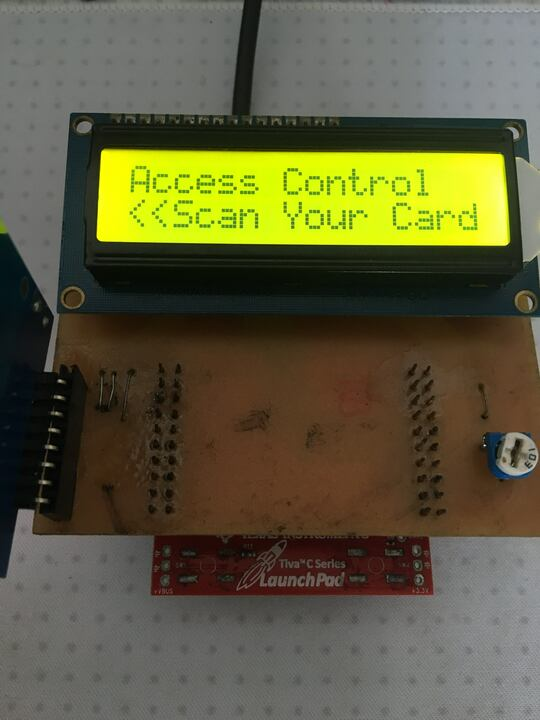
\includegraphics[scale=0.3]{images/mfrc522_default.jpg}
\caption{Kết quả hệ thống MFRC522 - Hệ thống ở trạng thái mặc định}
\label{fig:rc522_default}
\end{figure}

\begin{figure}[ht]
\centering
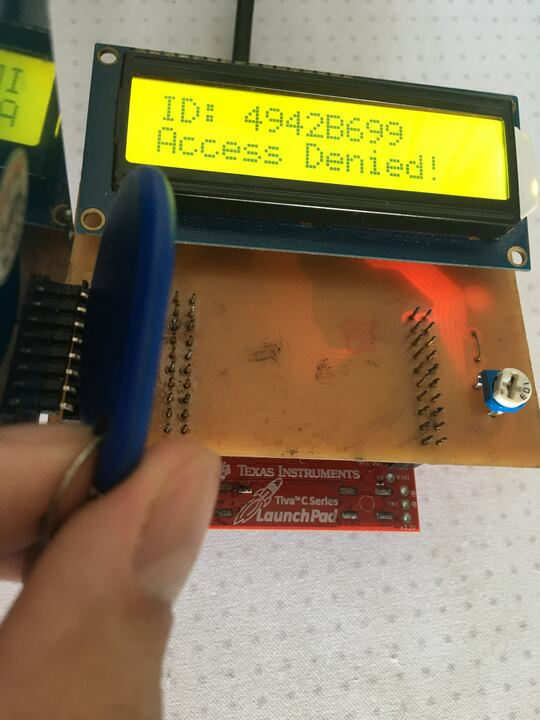
\includegraphics[scale=0.3]{images/mfrc522_tag.jpg}
\caption{Kết quả hệ thống MFRC522 - Sử dụng tag đi kèm}
\label{fig:rc522_tag}
\end{figure}

\begin{figure}[ht]
\centering
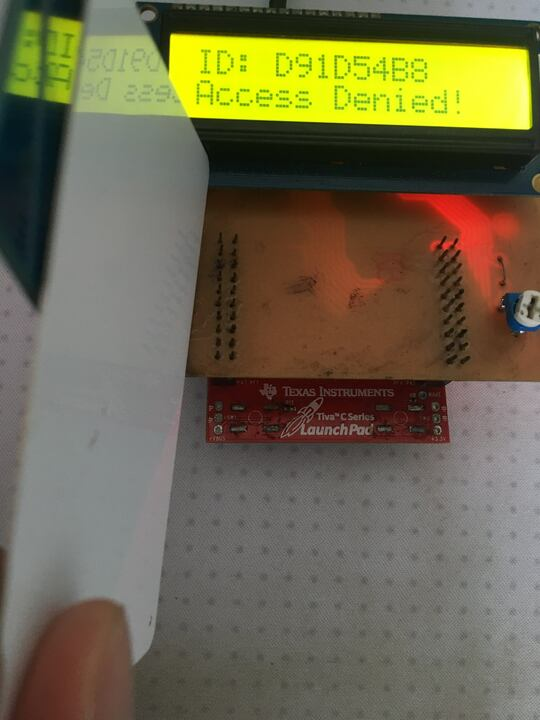
\includegraphics[scale=0.3]{images/mfrc522_card.jpg}
\caption{Kết quả hệ thống MFRC522 - Sử dụng card đi kèm}
\label{fig:rc522_card}
\end{figure}

\begin{figure}[ht]
\centering
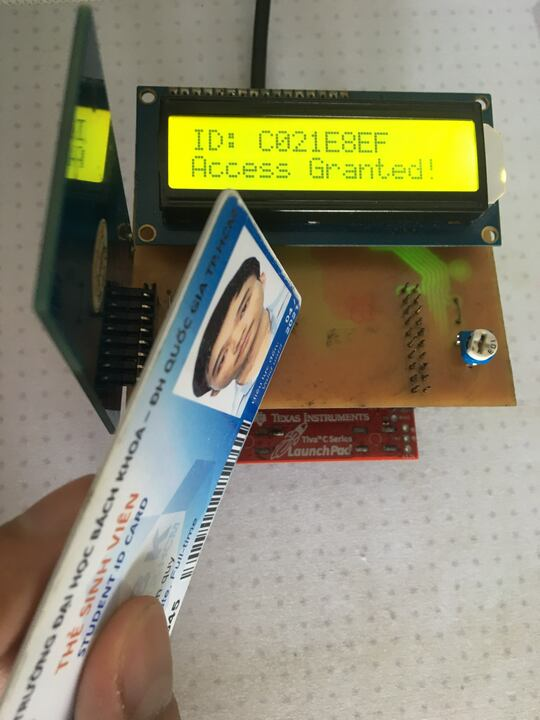
\includegraphics[scale=0.3]{images/mfrc522_student.jpg}
\caption{Kết quả hệ thống MFRC522 - Sử dụng thẻ sinh viên}
\label{fig:rc522_student}
\end{figure}

\clearpage
\subsection{Sử dụng một crate giải thuật cờ vua no-std trên kit Tiva C}\label{lbl:rust_chess}
Một trong những điểm mạnh của Rust là các crate no-std có thể được sử dụng trên bất kỳ môi trường nào như đã giới thiệu ở phần trước.
Vì vậy, ở phần này, em thực hiện sử dụng một crate giải thuật cờ vua \mintinline{bash}{chess-engine} \cite{rust_chess_engine} mô phỏng một hệ thống đánh cờ vua blindfolded (không bàn cờ) đơn giản để chứng minh điều này.
Trong phần này, em cũng sử dụng thêm một module bàn phím 4x4 để tăng tính tương tác với người dùng.
Crate thực hiện giải thuật cờ vua này tương đối đơn giản, dựa trên hai giải thuật Minimax \cite{minimax_chess_programming} và Alpha-Beta Pruning \cite{alpha_beta_chess_programming}.
Người đọc có thể tham khảo về giải thuật này ở phần tài liệu tham khảo.

Để thực hiện demo cho phần này, em thực hiện thiết lập một vị trí đơn giản như hình \ref{chess:start_fen}.
Ở đây, người chơi (điều khiển quân trắng) sẽ đi nước Qc6, cố tình tạo một thời cơ để cho máy tính (điều khiển quân đen) chơi một tactic 1. Bh2+ Kxh2 2. Qxc6.

Nội dung của chương trình người đọc có thể tham khảo ở phần phụ lục \ref{lbl:appendix_rust_chess} (trang \pageref{lbl:appendix_rust_chess}).


\begin{figure}[ht]
\centering
\newchessgame
\def\fenstart{2kr2nr/p1p2ppp/1p1b2q1/3N4/2Q5/4B3/PPP2PPP/R3R1K1 w - - 4 16}
\chessboard[smallboard, setfen=\fenstart]

\mainline{1. Qc6??}
\caption{Ví trí ban đầu để thử nghiệm giải thuật cờ vua}
\label{chess:start_fen}
\end{figure}

\begin{figure}[ht]
\centering
\newchessgame
\def\fenbotezgambit{2kr2nr/p1p2ppp/1pQb2q1/3N4/8/4B3/PPP2PPP/R3R1K1 b - - 5 16}
\chessboard[smallboard, setfen=\fenbotezgambit]

\mainline{1. Bxh2+ Kxh2 2. Qxc6}
\caption{Ví trí sau khi đi nước Qc6 để máy tính bắt đầu tính toán}
\label{chess:botez_gambit}
\end{figure}

Một vài hình về kết quả thực hiện có thể xem ở các hình \ref{fig:chess_init}, \ref{fig:chess_c4c6}, \ref{fig:chess_wait_move2}, \ref{fig:chess_g1h2}, \ref{fig:chess_end}, \ref{fig:chess_illegal}.

\begin{figure}[ht]
\centering
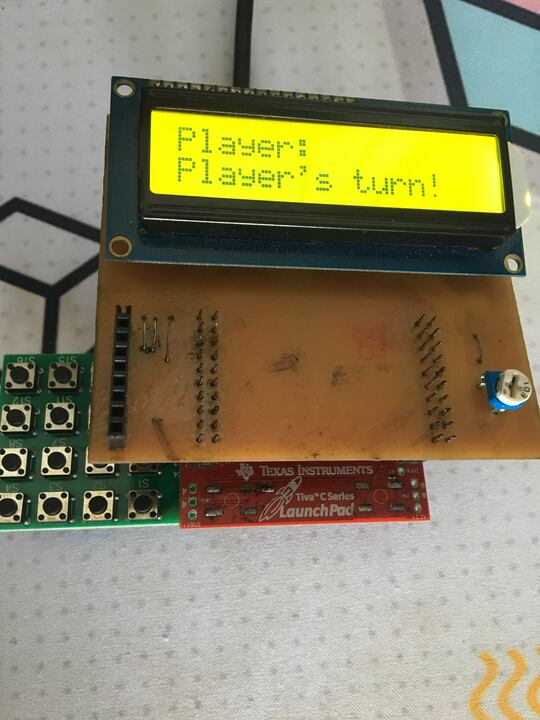
\includegraphics[scale=0.3]{images/chess_init.jpg}
\caption{Kết quả hệ thống MFRC522 - Hệ thống ở trạng thái mặc định như ở hình \ref{chess:start_fen}}
\label{fig:chess_init}
\end{figure}

\begin{figure}[ht]
\centering
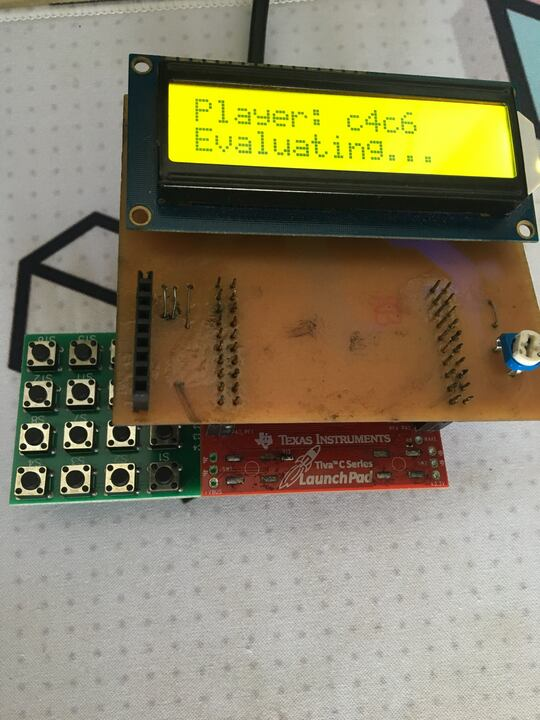
\includegraphics[scale=0.3]{images/chess_c4c6.jpg}
\caption{Kết quả hệ thống MFRC522 - Hệ thống đang giải nước Qc6}
\label{fig:chess_c4c6}
\end{figure}

\begin{figure}[ht]
\centering
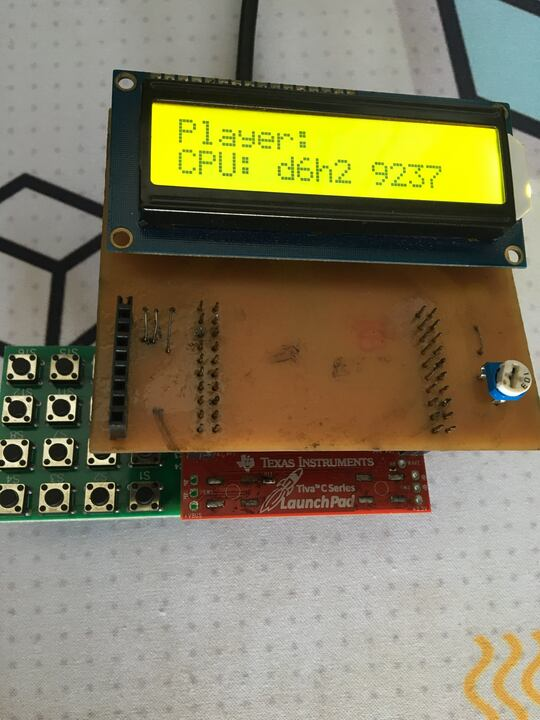
\includegraphics[scale=0.4]{images/chess_wait_move2.jpg}
\caption{Kết quả hệ thống MFRC522 - Hệ thống sau khi giải xong nước Qc6}
\label{fig:chess_wait_move2}
\end{figure}

\begin{figure}[ht]
\centering
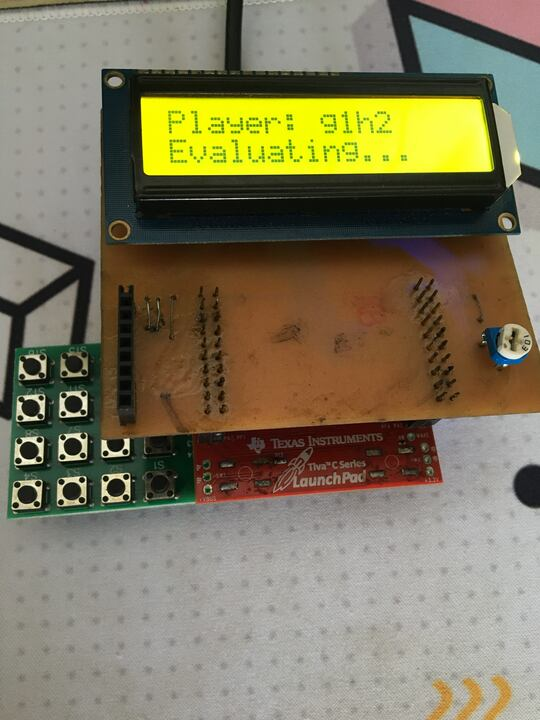
\includegraphics[scale=0.4]{images/chess_g1h2.jpg}
\caption{Kết quả hệ thống MFRC522 - Hệ thống đang giải nước Bxh2}
\label{fig:chess_g1h2}
\end{figure}

\begin{figure}[ht]
\centering
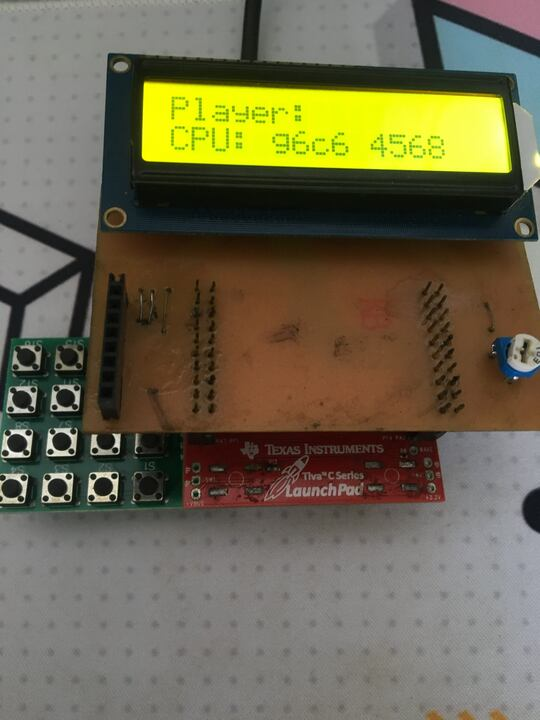
\includegraphics[scale=0.4]{images/chess_end.jpg}
\caption{Kết quả hệ thống MFRC522 - Hệ thống sau khi giải xong nước Bxh2}
\label{fig:chess_end}
\end{figure}

\begin{figure}[ht]
\centering
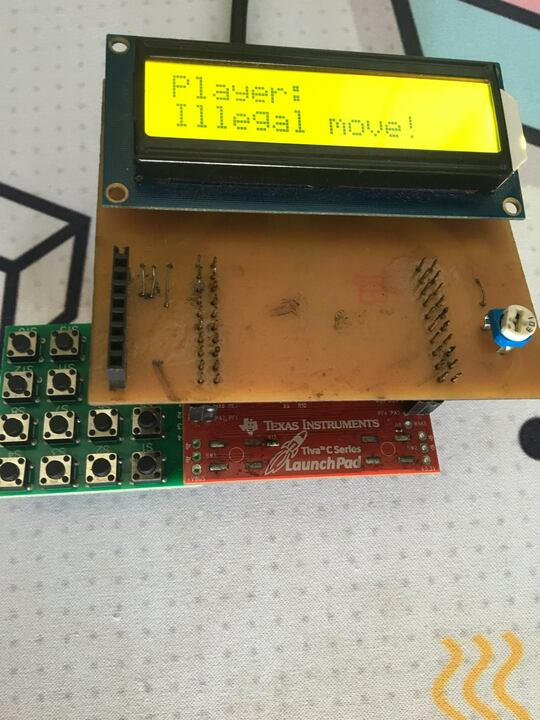
\includegraphics[scale=0.4]{images/chess_illegal.jpg}
\caption{Kết quả hệ thống giải thuật cờ vua - Người chơi đi nước không hợp lệ}
\label{fig:chess_illegal}
\end{figure}

\clearpage
\subsection{Sử dụng crate RTIC viết hệ thống real time sử dụng ngắt}\label{lbl:rust_rtic}
Một trong những cơ chế quan trọng trong việc viết những phần mềm nhúng nâng cao đó là sử dụng tính năng ngắt của vi điều khiển.
Trong phần này, em thực hiện sử dụng crate RTIC \cite{rtic_website} để viết một hệ thống nhúng real time sử dụng ngắt.

Hệ thống real time này là một hệ thống đơn giản, kết hợp các kiến thức đã thực hiện ở các phần \ref{lbl:rust_blinky} (trang \pageref{lbl:rust_blinky}), \ref{lbl:rust_peripheral} (trang \pageref{lbl:rust_peripheral}), \ref{lbl:rust_mfrc522} (trang \pageref{lbl:rust_mfrc522}) trước và kết hợp thêm một vài ví dụ nhỏ để mô tả chức năng scheduler của RTIC.

Hệ thống này gồm 5 tác vụ (tasks) trong đó 3 tác vụ là ngắt software và 2 tác vụ là ngắt hardware.
Hệ thống có các tính năng như sau:
\begin{itemize}
    \item Tác vụ LED: Nháy LED xanh dương sau mỗi 1s. Tương tự như phần \ref{lbl:rust_blinky} (trang \pageref{lbl:rust_blinky}), tuy nhiên ở đây sử dụng tính năng scheduler của RTIC.
    \item Tác vụ UART hardware: Thực hiện ngắt và đọc dữ liệu truyền đến kit qua UART. Tương tự hệ thống ở phần \ref{lbl:rust_peripheral} (trang \pageref{lbl:rust_peripheral}).
    \item Tác vụ LCD: Sau mỗi 0.5s tăng 1 vào một biến (ở đây là biến \mintinline{bash}{lcd_counter}) và xuất ra màn hình LCD.
    \item Tác vụ MFRC522: Thực hiện ngắt và đọc giá trị của thẻ RFID khi có thẻ được quét. Tương tự như hệ thống ở phần \ref{lbl:rust_mfrc522} (trang \pageref{lbl:rust_mfrc522}).
    \item Tác vụ UART software: Sau mỗi 2s xuất ra UART các giá trị của hệ thống như \mintinline{bash}{lcd_counter} và số thẻ đã đọc được ở tác vụ MFRC522 (biến \mintinline{bash}{card_counter}).
\end{itemize}

Nội dung của chương trình người đọc có thể tham khảo ở phần phụ lục \ref{lbl:appendix_rust_rtic} (trang \pageref{lbl:appendix_rust_rtic}).
Một vài hình về kết quả thực hiện có thể xem ở các hình \ref{fig:rtic_init}, \ref{fig:rtic_tag}, \ref{fig:rtic_card}, \ref{fig:rtic_student}, \ref{fig:rtic_uart}.

\begin{figure}[ht]
\centering
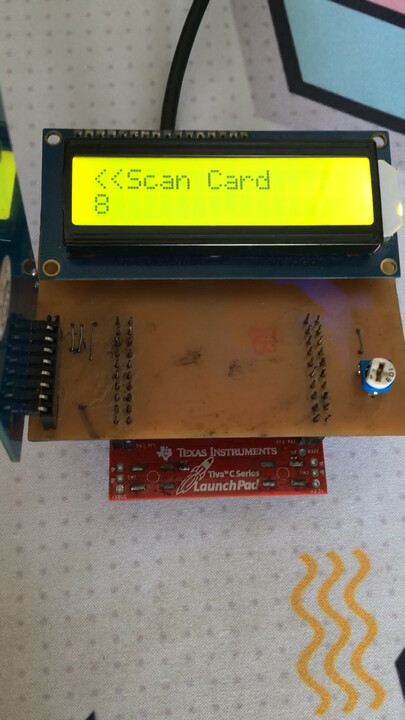
\includegraphics[scale=0.3]{images/rtic_init.jpg}
\caption{Kết quả hệ thống RTIC - Hệ thống ở trạng thái ban đầu}
\label{fig:rtic_init}
\end{figure}

\begin{figure}[ht]
\centering
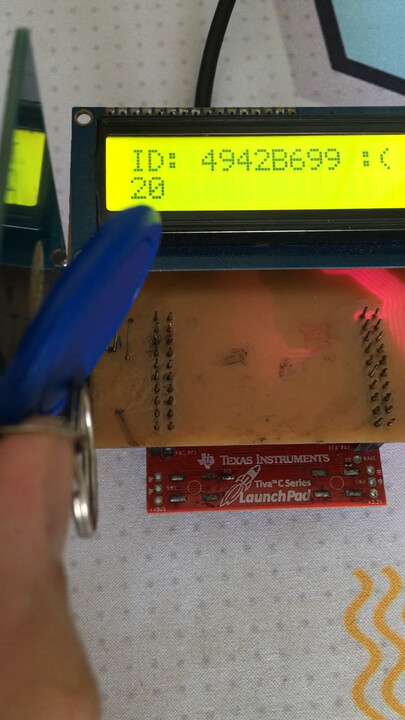
\includegraphics[scale=0.4]{images/rtic_tag.jpg}
\caption{Kết quả hệ thống RTIC - Hệ thống khi quét tag}
\label{fig:rtic_tag}
\end{figure}

\begin{figure}[ht]
\centering
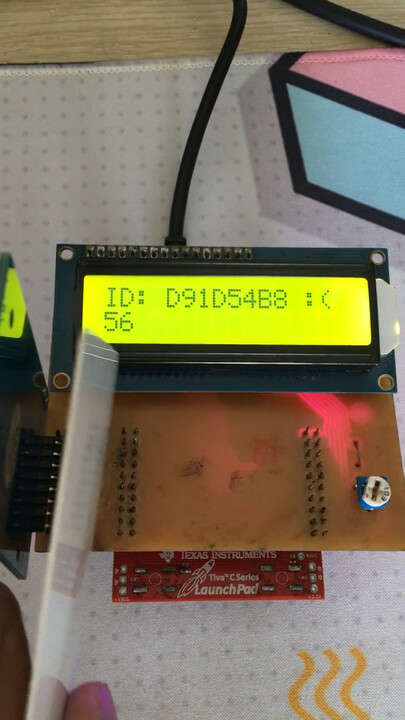
\includegraphics[scale=0.4]{images/rtic_card.jpg}
\caption{Kết quả hệ thống RTIC - Hệ thống khi khi quét card}
\label{fig:rtic_card}
\end{figure}

\begin{figure}[ht]
\centering
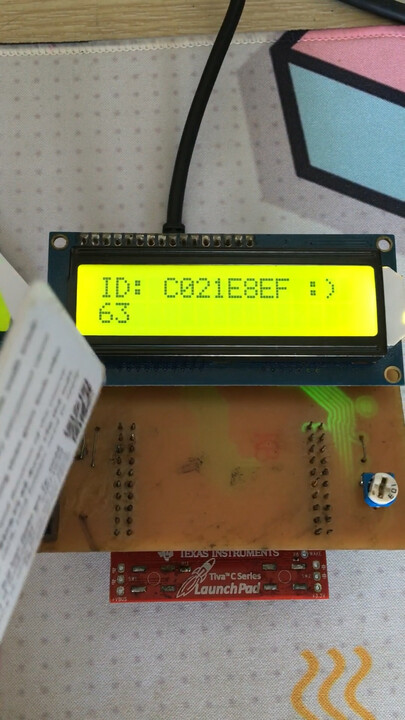
\includegraphics[scale=0.4]{images/rtic_student.jpg}
\caption{Kết quả hệ thống RTIC - Hệ thống khi quét thẻ sinh viên}
\label{fig:rtic_student}
\end{figure}

\begin{figure}[ht]
\centering
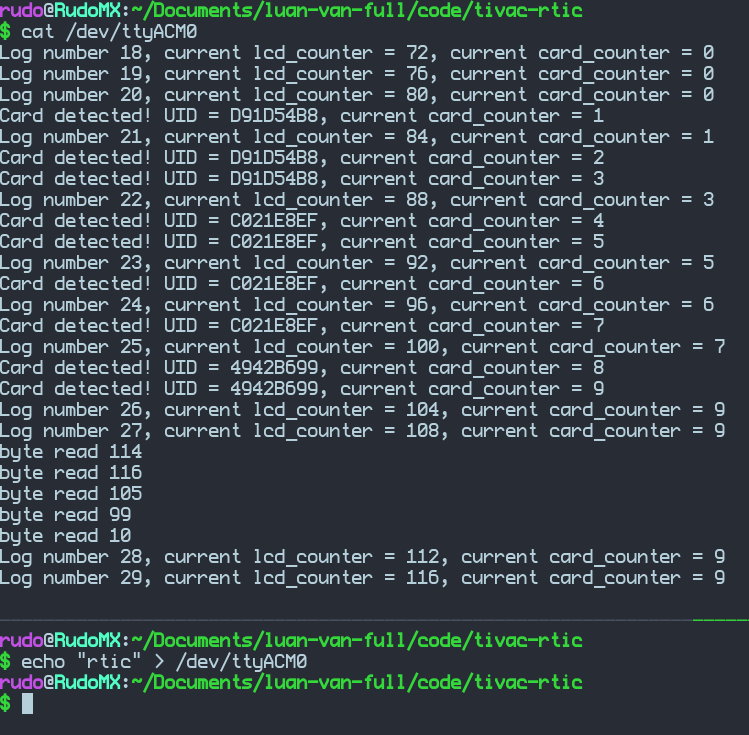
\includegraphics[scale=0.5]{images/rtic_uart.png}
\caption{Kết quả hệ thống RTIC - Hệ thống ghi và đọc cổng UART}
\label{fig:rtic_uart}
\end{figure}

\clearpage
Trong các phần thực hiện hệ thống thì phần sử dụng crate RTIC này, em gặp nhiều trục trặc về kỹ thuật nhất.
Các vấn đề trực trặc kỹ thuật này xuất phát từ cả hai crate đó là RTIC, cũng như là HAL chưa đầy đủ của kit Tiva C.
Một số khó khăn có thể được liệt kê ra như sau:
\begin{itemize}
    \item HAL của Tiva C ở thời điểm viết bài chưa hỗ trợ ngắt trực tiếp UART cũng như SSI.
        Hiện tại hệ thống sử dụng ngắt GPIO để thay thế, vì vậy bị mất đi các chân GPIO sử dụng để ngắt khi thực hiện điều này.
    \item HAL của Tiva C hiện tại chỉ có một cách tạo biến delay duy nhất đó là sử dụng SysTick, tuy nhiên RTIC lại sử dụng SysTick cho monotonic scheduler.
        Vì vậy người dùng monotonic scheduler phải thực hiện viết cách tạo delay khác.
        Ở đây em chọn cách sử dụng countdown timer trên kit để tạo delay.
    \item RTIC sử dụng các phương pháp quản lý tài nguyên hệ thống cũng như switch task tương đối khác so với hệ thống RTOS quen thuộc nên đã gây một số hiểu lầm trong quá trình thực hiện hệ thống.
\end{itemize}

Tuy nhiên về cơ bản thì việc thực hiện hệ thống sử dụng crate RTIC là tương đối đơn giản và dễ dàng.
Crate RTIC kết hợp chặt chẽ với hệ thống ownership của Rust ngăn chặn được nhiều lỗi trong hệ thống ngắt nói chung như datarace thông qua hệ thống resource lock của mình.

\chapter{Kết luận}
\section{Đánh giá kết quả}
Nói chung, em đã có một trải nghiệm mới và tốt khi thực hiện một hệ thống nhúng sử dụng Rust trong suốt quá trình thực hiện đề tài này.
Trong môi trường nhúng tuy ta không thể sử dụng được thư viện std của Rust gồm rất nhiều tính năng mạnh mẽ, chất lượng, v.v.. nhưng kể cả bỏ qua thư viện chuẩn, sử dụng thư viện core của Rust, cùng với hệ thống ownership mới mẻ đã tạo nên một bộ công cụ hỗ trợ công việc thực hiện một hệ thống nhúng một cách dễ dàng và hiệu quả.

Hệ sinh thái nhúng của Rust được xây dựng một cách hiệu quả, an toàn ngay từ gốc đã góp phần không nhỏ trong việc sử dụng ngôn ngữ này trong hệ thống nhúng một cách hiệu quả và dễ dàng hơn. Ngoài ra, nó cũng góp phần tạo nên tính portability rất cao cho mã nguồn Rust. Hơn nữa, cũng vì tính portability cao này mà ta có thể dễ dàng học được cách viết các mã nguồn chất lượng cao từ các crate trong hệ sinh thái của Rust.

Tuy hệ sinh thái nhúng của Rust còn nhiều thiếu sót nhưng trong những năm tiếp theo khi Rust nhận được nhiều sự chú ý từ các tập đoàn, công ty chuyên về lập trình nhúng thì trong tương lai các thiếu sót này sẽ dần được bổ sung, hoàn thiện. Trong tương lai gần, có thể hệ sinh thái nhúng của Rust sẽ phát triển đủ mạnh để dần chiếm được thị trường nhúng, nơi mà C đang làm chủ ở mọi mặt.

Thông qua việc thực hiện năm ví dụ có độ khó từ đơn giản đến tương đối phức tạp ở phần trên, có thể khẳng định rằng Rust hoàn toàn có thể được sử dụng để thực hiện một hệ thống nhúng trong thực tế trong hôm nay một cách dễ dàng và thuận tiện.
Các hệ thống này được nhận các lợi ích từ hệ thống ownership system, giúp chúng tránh được nhiều lỗi thường gặp trong hệ thống C ngay trong lúc biên dịch chương trình.

Mã nguồn của hệ thống có thể được quản lý, debug, test, v.v.. một cách dễ dàng sử dụng công cụ \mintinline{bash}{cargo} đi kèm với ngôn ngữ.
Các hệ thống cũng được kiểm tra qua Github CI một cách thuận tiện, không gặp trở ngại.
Các công cụ khác hỗ trợ cho việc thiết kế và thực hiện ngôn ngữ Rust như IntelliJ hay Esclipse RustDT đang được phát triển một cách nhanh chóng.
Trong tương lai gần, các bộ công cụ này có thể trở thành cánh tay phải đắc lực cho các nhà phát triển ngôn ngữ Rust.

Một điểm yếu lớn trong quá trình thực hiện đề tài mà em rút ra được là: vì Rust là một ngôn ngữ còn mới, vì vậy tài liệu học tập cũng như các đề tài thực hiện sử dụng ngôn ngữ này là tương đối hạn chế.
Một người lập trình muốn thử nghiệm ngôn ngữ Rust có thể sẽ gặp phải nhiều vướng mắt trong quá trình thực hiện.
Tuy nhiên, cộng đồng những người lập trình Rust rất ưu ái đối với những câu hỏi về ngôn ngữ, cũng như cách thực hiện viết các mã nguồn chất lượng cao đã giúp em tự tin hơn trong quá trình thực hiện đề tài này.

\section{Hướng phát triển}
Rust là một ngôn ngữ mới nhưng có tiềm năng phát triển rất lớn, kể cả trong mảng lập trình nhúng.
Để góp phần thúc đẩy sự phát triển này, em đề xuất một số hướng như sau:
\begin{enumerate}
    \item Mở rộng tầm ảnh hưởng cũng như nhận thức của mọi người về ngôn ngữ mới này:
        Rust càng nhận được nhiều sự quan tâm từ mọi người, cũng như các công ty, tập đoàn chuyên về lập trình nhúng thì nguồn lực đổ vào để phát triển ngôn ngữ này sẽ càng lớn hơn.
    \item Thúc đẩy sự phát triển của các bộ công cụ hỗ trợ cho việc thiết kế một hệ thống Rust:
        Một bộ công cụ hỗ trợ tốt chính là chìa khóa để có được trải nghiệm tốt nhất khi thử nghiệm một ngôn ngữ mới.
    \item Hỗ trợ, bổ sung thêm các crate chất lượng cao:
        Hệ sinh thái nhúng của Rust còn tương đối non nớt vì vậyviệc bổ sung thêm các crate là điều cực kỳ cần thiết.
    \item Hỗ trợ viết thêm các tài liệu học tập cho Rust:
        Như đã phân tích ở phần trên, tài liệu học tập Rust, đặc biệt là trong mảng lập trình nhúng là tương đối hạn chế.
        Vì vậy, hỗ trợ viết các tài liệu học tập này sẽ góp phần không nhỏ trong việc thúc đẩy sự phát triển của Rust.
\end{enumerate}


\backmatter
\phantomsection
\addcontentsline{toc}{chapter}{Tài liệu tham khảo}
\nocite{*} % Basically don't cite anything but print all of the stuff in bibliography file out
\emergencystretch=1em
\printbibliography[title=Tài liệu tham khảo]
% This is the default way to handle bibliography
%\bibliographystyle{ieeetr}
%\bibliography{uni}

%----- APPENDIX (PHU LUC) -----
% Detailed schematic, extra information, source code and other shit are put in here
\end{document}
